%%%%%%%%%%%%%%%%%%%%%%%%%%%%%%%%%%%%%%%%%%%%%%%%%%%%%%%%%%%%%%%%%%%
%%%%%%%%%%%%%%%%%%%%%%% DEUXIEME PARTIE %%%%%%%%%%%%%%%%%%%%%%%%%%%
%%%%%%%%%%%%%%%%%%%%%%%%%%%%%%%%%%%%%%%%%%%%%%%%%%%%%%%%%%%%%%%%%%%

\part{Normalisation, enrichissements et extraction d'informations: une chaîne de traitement pour des données semi-structurées}

\chapter{Faire sens d'un corpus complexe: homogénéisation des données et extraction d'informations}
\chaptermark{Faire sens d'un corpus complexe}

\section{Homogénéiser et normaliser un corpus complexe}
Cette section s'intéresse à la manière dont les fichiers \tei{} sont traités afin de pouvoir ensuite en extraire des informations. C'est directement grâce la structure des entrées (et grâce à la nature \enquote{semi-structurée} des catalogues) qu'est possible le traitement automatisé des documents.

\subsection{Pourquoi chercher à normaliser le corpus?}
La question mérite d'être posée: des étapes de post-traitement du corpus sont nécessaires pour pouvoir en extraire des informations et pour pouvoir donc en faire sens; cependant ce processus peut également impacter la nature du texte et ses significations. Tout comme l'édition \tei{} originelle est un processus sélectif, le traitement des documents encodés est lui un processus sélectif: certaines informations contenues par l'encodage sont privilégiées aux dépens d'autres. Il s'agit ici d'expliciter ces choix (travailler sur les prix, les formats et dimensions des manuscrits plutôt que sur leur sujet) et de les justifier. Cette section s'attache donc à rappeler les questions de recherche qui sous-tendent la normalisation des documents (ajouter plus de structure au document \tei{} pour l'exploiter plus facilement, uniformiser la notation des tailles et des dimensions des documents...).

\subsection{Comment normaliser le corpus tout en préservant sa valeur documentaire?}
Ici, on s'intéresse à la manière dont la \tei{} est mise à profit pour enrichir le corpus tout en conservant le contenu textuel des catalogues. Les différentes étapes de normalisation sont également rappelées (ce travail n'étant pas au cœur de mon stage, il s'agira plutôt d'un rappel que d'une présentation technique détaillée).

\section{Faire sens du corpus: extraction d'informations et fouille de texte}
Ici sont décrits le processus et les objectifs de l'extraction d'informations à partir des fichiers \tei{}. C'est à partir de cette opération d'extraction que sont construites les visualisations, qui permettent une approche graphique du corpus et une meilleure compréhension de celui-ci.

\subsection{Extraire des informations au niveau des entrées}
Des données sont extraites pour chaque entrée de catalogue (un travail largement effectué par A. Bartz, que j'ai légèrement mis à jour) : prix (dans la monnaie de l'époque et en francs constants), date de vente normalisée, nom de l'auteur.ice et description du manuscrit... L'extraction d'informations pour les entrées individuelles permet surtout de faire une réconciliation des manuscrits vendus (c'est à dire, de retrouver les items vendus plusieurs fois).

\subsection{Extraire des informations au niveau des catalogues}
Un second processus d'extraction produit des données pour chaque catalogue de vente: titre du catalogue, date de vente, nombre d'items vendus, prix minimum, inférieur et maximum, prix moyen et médian, variance... Ce processus met l'accent sur une approche statistique et économique du corpus, qui permettra d'étudier l'évolution du cours et du volume du marché des manuscrits (nombre d'items en vente, évolution des prix).

\subsection{Vers une approche économique du corpus: la conversion automatique des prix en francs constants}
En même temps que ces processus d'extraction d'informations, un script de conversion des monnaies (françaises et étrangères) en francs constants 1900 a été élaboré. En annulant l'effet de l'inflation, les francs constant permettent d'étudier l'évolution réelle des prix.


\chapter{Vers une étude des facteurs déterminant le prix des documents: alignement des entrées du catalogue avec \wkd{} et exploitation de données normalisées}
\chaptermark{Vers une étude...}
Ce chapitre est construit autour d'une question de recherche: comment produire des informations exploitables pour une étude économétrique à partir d'un corpus textuel semi-structuré? Un des objectifs du projet est de faire l'étude des facteurs déterminant le prix d'un manuscrit. Pour faire cette étude, il faut obtenir, pour chaque entrée du catalogue, un certain nombre d'informations normalisées. Le travail d'extraction de données présentes dans les catalogues a déjà été fait par de précédent.e.s stagiaires. Ces données sont principalement quantitatives: prix des manuscrits, dimensions et nombre de pages, date de création. Il est nécessaire de compléter les informations par des données qualitatives et d'enrichir les données disponibles avec des sources extérieures. Pour ce faire, il a été choisi d'aligner le nom des auteur.ice.s des manuscrits avec des identifiants \wkd{}; dès lors que l'on a un identifiant \wkd{}, il est possible de récupérer automatiquement des informations sur les personnes via \sparql. Le choix de travailler uniquement sur les noms, et non sur la description des documents, a deux motivations:
\begin{itemize}
	\item Les noms de personnes (et la manière dont elles sont décrites) constituent la partie la plus normalisée des documents. La description des manuscrits est plutôt en \enquote{texte libre}. Dans la continuité avec le reste du projet, nous sommes resté dans une approche \enquote{basse technologie}, qui consiste à s'appuyer majoritairement sur des solutions techniquement simples. C'est pourquoi nous avons préférer traiter les noms avec des tables de correspondance\footnote{C'est à dire, des tables qui permettent de normaliser la manière dont les informations figurent dans les catalogues, et donc de remplacer des termes \enquote{vernaculaires} par leurs équivalents utilisés par \wkd{}} et des \rgxpl{}, plutôt que de faire du TAL sur la description des documents.
	\item Toutes les informations \enquote{simples} (données quantitatives facilement normalisables: dates etc.) ont déjà été extraites des descriptions des manuscrits.
\end{itemize}

Ce travail d'enrichissement a été fait en deux temps. 

La première étape, et la plus difficile, est l'alignement avec \wkd{}. Cela demande d'extraire un ensemble d'informations à partir du nom de la personne et de la description de celle-ci. Parmi les informations extraites: nom, prénom, titre de noblesse, occupation, dates de vie et de mort. À partir de ces informations, stockées dans un dictionnaire, un algorithme construit successivement différentes chaînes de caractères pour lancer des recherchers en plein texte sur l'\api{} de \wkd{}. L'objectif est que le premier résultat recherché sur \wkd{} soit correct. Sur un jeu de test, le \gls{score F1} obtenu est de 68\%. Un relecture \enquote{manuelle} des résultats est donc nécessaire.

La deuxième étape, nettement plus simple, consiste à lancer des requêtes \wkd{} sur les identifiants récupérés afin de récupérer des informations sur les auteur.ice.s des manuscrits (cette partie du travail est encore en cours) pour enrichir nos données.

Une fois ce travail effectué, l'enrichissement des données à proprement parler est possible: les fichiers \tei{} sont mis à jour pour ajouter les identifiants \wkd{}. Ainsi, il est possible de faire le lien entre les entrées de catalogues dans des fichiers \xml{} et les données issues de requêtes \sparql{}, stockées dans un \json.


\section{Questions introductives: pourquoi et comment s'aligner avec \wkd{} ?}
\sectionmark{Questions introductives}
Cette section, introductive, répond à des questions évidentes mais essentielles: elles permettent de mettre au clair l'intérêt et les (multiples) difficultés dans l'alignement avec \wkd{}.

\subsection{Pourquoi s'aligner avec des entités externes?} 

L'alignement avec \wkd{} a pour objectif principal de mieux comprendre les déterminants du prix des manuscrits sur le marché du \scl{XIX}. Mais pourquoi passer par un alignement avec \wkd{}? 

Pour étudier les déterminants du prix d'un manuscrit, il faut établir la relation entre la variable dont la valeur est étudiée (le prix d'un manuscrit) et un ensemble d'autres facteurs (qui a écrit un manuscrit, quelles sont ses dimensions, de quand date le document...). En d'autres termes, il faut étudier le comportement d'une variable en fonction d'autres variables. En économétrie, cette opération s'appelle le calcul de régressions linéaires. La variable étudiée (le prix) est dite la variable expliquée; les facteurs déterminant la valeur de cette variable sont dites \enquote{variables explicatives}\footcite{noauthor_regression_2022}. Cependant, cette opération est loin d'être anodine: il faut d'abord identifier les variables pertinentes, et ensuite trouver un moyen de les quantifier. Deux difficultés se présentent pour alors.

Premièrement, il faut pouvoir quantifier les variables expliquées pour calculer des régressions linéaires. Il est possible de leur assigner une valeur numéraire (ce qui est aisé pour les informations quantitatives des catalogues: la date de l'écriture d'un manuscrit, ses les dimensions). Une autre possibilité est de quantifier la présence ou non d'une variable: mention d'un.e destinataire ou du contenu d'un manuscrit. Cependant, ces approches quantitatives ne permettent pas de quantifier des informations complexes, comme la célébrité des auteur.ice.s, ou encore si un manuscrit porte sur un évènement historique ou biographique important (le manuscrit d'un texte célèbre, par exemple, pourrait avoir une valeur particulières). Ces informations sont parfois être présentes dans les catalogues; elles peuvent aussi être connues des lecteur.ice.s d'aujourd'hui et des acheteurs et acheteuses de l'époque. Il n'existe cependant pas de méthodes faciles pour détecter ou quantifier la célébrité d'une personne, ou l'importance d'un sujet.

Une deuxième difficulté découle justement de la part d'implicite qu'il y a dans les catalogues. Les descriptions des items vendus sont brèves, et comprendre ce qui fait la valeur d'un manuscrit demande aux acheteur.euse.s d'avoir des références culturelles et historiques: celles-ci permettent d'identifier l'auteur.ice ou le sujet, et donc pour comprendre la valeur d'un manuscrit. Dans le cadre du projet \mssktb{}, les entrées de catalogues sont traitées par une machine qui, en toute logique, ne dispose pas de ces références. La compréhension qualitative des entrées de catalogues n'est donc pas compatible avec l'approche par lecture distante du projet. Pour éviter de perdre ces informations qualitatives essentielles, il est donc nécessaire de trouver un moyen de quantifier le qualitatif.

En bref, la question est: comment faire la différence entre une lettre de La Rochefoucauld (\ref{fig:rochefoucauld}), vendue 200 francs, et la deuxième (\ref{fig:villars}), vendue à 30 francs? Le problème est un problème de lecture. Une observation de la description des lettres par un être humain comme par une machine peuvent identifier des éléments semblables dans le texte: les deux lettres sont écrites par des ducs; l'une est une \enquote{Très-belle lettre} (\ref{fig:rochefoucauld}), l'autre est une \enquote{Lettre intéressante} (\ref{fig:villars})\footnote{Ce sont des informations qui se retrouvent souvent, et il est donc possible d'écrire un programme qui les relève automatiquement}. Bien que les lettres partagent des attributs, il y a une forte différence de prix entre les deux manuscrits. Un.e lecteur.ice peut trouver une raison à cette différence de prix: La Rochefoucauld et Madeleine de Scudéry n'ont pas le même statut que le duc de Villars. Un regard humain peut donc interpréter un prix et déterminer une valeur en s'appuyant sur ses connaissances. La lecture est qualitative et s'appuie sur de l'implicite, ce qui n'est pas possible pour une machine: formellement, rien ne distingue un nom d'un autre; lorsqu'un programme \enquote{lit} un texte, il ne peut pas s'appuyer sur ses connaissances pour déterminer ce qu'un nom signifie, ce à quoi il fait référence.

\begin{figure}[h!]
	\centering
	\begin{subfigure}{0.8\textwidth}
		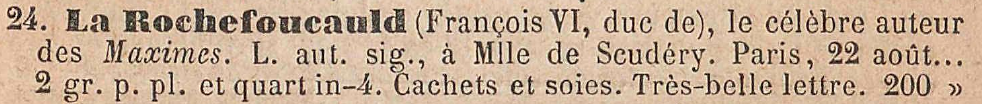
\includegraphics[width=\textwidth]{img/cat_000372_e24.png}
		\caption{Une lettre écrite par La Rochefoucauld vendue à 200 francs.}
		\label{fig:rochefoucauld}
	\end{subfigure}
	\begin{subfigure}{0.8\textwidth}
		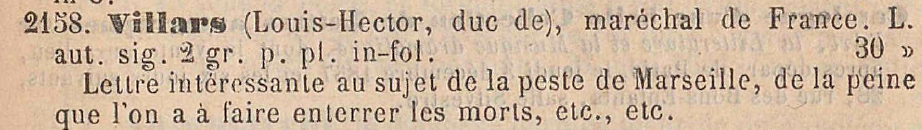
\includegraphics[width=\textwidth]{img/cat_000382_e2158.png}
		\caption{Une lettre écrite par Louis-Hector Villars vendue à 30 francs.}
		\label{fig:villars}
	\end{subfigure}
	\caption{Deux exemples de lettres}
\end{figure}

Pour analyser efficacement la variable \enquote{prix}, il faut pourtant pouvoir, dans une certaine mesure, comprendre les informations implicites et qualitatives contenues dans les catalogues. Le parti pris a donc été de construire le socle de connaissance qui manque à une machine, en s'alignant avec \wkd{} et en s'en servant pour enrichir nos données. Le choix a été fait de ne s'aligner avec \wkd{} que pour certaines parties des entrées de catalogue. Pour rappel, voici leur structure (\ref{code:tei_item}):

\begin{listing}
	\inputminted[linenos, breaklines, tabsize=4]{xml}{code/tei_item.xml}
	\caption{Représentation \xmltei{} d'une entrée de catalogue}
	\label{code:tei_item}
\end{listing}


Les entrées de catalogue contiennent beaucoup d'informations qualitatives, qui pourraient avoir une influence sur le prix du manuscrit: ici par exemple, la description du contenu de la lettre dans le \tnote{}; il est également souvent fait mention du ou de la destinataire. Cependant, l'alignement avec \wkd{} n'a pas été fait avec l'intégralité des entrées. C'est seulement le contenu du \tname{} qui a été aligné avec \wkd{}, à l'aide des informations contenues dans le \ttrait{}. Le \tdesc{} a déjà fait l'objet d'un grand travail de normalisation et d'extraction d'informations; un alignement avec des sources externes n'aurait donc pas une très grande plus-value. L'élément \tnote{} contient souvent des informations intéressantes, puisque c'est là qu'est décrit le contenu d'un manuscrit. Cependant, cet élément n'est pas toujours présent; son contenu est souvent écrit en langage naturel, non structuré, et contient des informations trop variées pour développer un traitement uniforme. Il est donc difficile de tirer parti de cet élément. Le \tname{} et son \ttrait{} sont les éléments les plus régulièrement présents; les informations qu'ils contiennent sont toujours les mêmes (nom d'une personne ou thème d'un manuscrit dans le \tname{}, description du \tname{} dans le \ttrait{}); enfin, ces deux éléments n'ont pas du tout été transformés dans le reste de la chaîne de traitement. Ils portent donc des informations qualitatives centrales pour produire des données exploitables dans une étude économétrique.

Le parti pris a donc été d'aligner avec des identifiants \wkd{} les noms contenus dans les balises \tname{} à l'aide des descriptions contenues dans les \ttrait{}; à partir de cet alignement a été constituée une base de données. Cela permet d'approximer une lecture \enquote{humaine} des items en vente: pour chaque auteur.ice, un certain nombre d'informations auront été récupérées pour mieux identifier la personne (ses occupations, son origine, ses dates de vie...). L'analyse du corpus s'appuit alors sur un bagage de connaissances qui permet d'appréhender par lecture distante l'importance d'une personne. Il devient alors envisageable de voir dans quelle mesure la mention d'une personne impacte le prix d'un manuscrit, et quels sont les facteurs biographiques déterminant dans l'établissement de la valeur. Pour revenir à l'exemple de La Rochefoucauld: à défaut de permettre de savoir qui il est, un alignement avec \wkd{} permet d'identifier son statut et sa place dans la culture française, en récupérant le nombre de ses publications ou encore les institutions dont il est membre.

\subsection{Pourquoi utiliser la base de connaissances \wkd{}?}
- brève intro sur wikidata avec le 1er article
- avantages: 
	-sparql endpoint facile (cf article 2 p.59), avec une seule ontologie (=/= DataBNF); 
	- distance entre l'entité et sa représentation linguistique, nature multilingue; 
	- présence d'une API et d'un Sparql endpoint qui permet de s'adapter à la méthode choisie pour cette étape
	- rdf compliance (cf p.56 du 2e article)
	- données produites directement, =/= DBPedia où elles sont scrapées
	- nature généraliste de la BDD; ça peut sembler surprenant, mais vu qu'on ne sait pas nécessairement avec quelles données on va travailler, ça peut être intéressant
- ensuite, fonctionnement technique de wkd, avec le modèle de données

\subsection{Quelle relation avec la résolution d'entités nommées d'entités nommées?}
blablabla à compléter plus tard

définition: \enquote{La tâche dite de résolution d’entités nommées (que nous désignerons par l’acronyme NEL pour Named Entity Linking) consiste à affecter automatiquement la bonne référence, l’identifiant de la ressource correspondante dans une base de connaissances ou bien NIL (l’absence de valeur), à une entité nommée préalablement identifiée dans un texte et étiquetée.}\footcite[p. 31]{carmen_evaluation_2016}

\subsection{Présentation générale de l'algorithme}
Construire un jeu de données issu de \sparql{} à partir de la manière dont une personne est nommée et décrite au \scl{XIX} n'est pas une opération anodine. La chaîne de traitement est donc assez complexe, comme le montre le schéma \ref{fig:wkdmain}. Cette chaîne de traitement peut être séparée en trois étapes.

\subsubsection{Étape 1 -- Extraction et structuration de données}
Premièrement, il s'agit d'aligner les entrées de catalogue avec des identifiants \wkd{}. Ceux-ci sont liés à des \enquote{entités} \wkd{}: des personnes, lieux et évènements décrits dans \wkd{} par un certain nombre de propriétés (date de naissance, lieu de résidences...). Cette première étape repose avant tout sur l'extraction et la traduction des données depuis les éléments \tname{} et \ttrait{}. Ce processus d'extraction permet de récupérer toutes les données pertinentes pour chaque entrée de catalogue et de les stocker dans un \gls{dictionnaire} structuré. Comme on le verra, la nature \enquote{semi-structurée} des entrées (ainsi qu'une bonne connaissance du corpus) permet de d'automatiser le processus d'extraction et de traduction des données par détection de motifs, sans avoir à passer par l'apprentissage machine: étant donné que les mêmes types d'informations sont toujours présentes et que les entrées suivent des modèles relativement proches, il est possible de s'appuyer sur la structure des entrées pour identifier  les informations pertinentes. L'extraction de données repose donc sur de la détection de motifs à l'aide d'\rgxpl{}: des récurrences sont repérées dans le texte et utilisées pour distinguer différentes informations (nom, prénom, titre de noblesse...). Pour appuyer l'usage d'expressions régulières par une méthode plus \enquote{qualitative} et précise, certains termes particuliers sont extraits et éventuellement traduits à l'aide de \glspl{table de conversion} (c'est-à-dire de \glspl{dictionnaire} qui associent à un terme dans le texte une version normalisée). 

\subsubsection{Étape 2 -- récupération d'identifiants \wkd{} via des recherches en plein texte à l'aide d'une \api{}}
Une fois les données du \tname{} et du \ttrait{} structurées en dictionnaire, elles sont utilisées pour lancer plusieurs recherches en plein texte sur le moteur de recherche de \wkd{}. Ces recherches sont faites automatiquement grâce à l'\api{} de \wkd{}. Pour maximiser les chances d'obtenir un identifiant valide, un algorithme a été conçu pour lancer plusieurs recherches à partir de chaque dictionnaire. La première recherche met bout-à-bout toutes les valeurs disponibles dans le dictionnaire. Ensuite, en fonction des paramètres de recherche disponibles dans le dictionnaire, différentes autres recherches sont lancées. Cet algorithme a été élaboré en menant de nombreux tests pour maximiser le taux de réussite, calculé sous la forme d'un \gls{score F1}.

\subsubsection{Étape 3 -- constitution d'un jeu de données à l'aide de \sparql{}}
Si l'étape d'alignement avec \wkd{} est la plus complexe, elle n'est qu'une étape préparatoire vers la constitution du jeu de données. En fait, récupérer les identifiants est seulement ce qui rend possible l'enrichissement en tant que tel: en lançant une requête \sparql{} sur tous ces identifiants, il est possible, pour chaque entité représentée par l'identifiant, de récupérer des informations depuis \wkd{} et donc de construire le jeu de données définitif. Pour cette étape, le processus est plus simple: les identifiants récupérés à la fin de l'étape précédente sont dédoublonnés (pour éviter de lancer plusieurs fois la même requête); ensuite une requête \sparql{} est initalisée et lancée chacun des identifiants. Les résultats sont traduits depuis les formats \json{} ou \xml{} retournés par \sparql{} sous forme de \json{} plus simple, et donc plus aisément manipulable. Le jeu de données est enregistré dans un fichier. Pour finir, les identifiants \wkd{} sont réinjectés aux catalogues \tei{}, afin de pouvoir faire le lien entre les catalogues et le jeu de données qui a été construit.

Cette chaîne de traitement étant lancée sur plus de 80000 entrées de catalogues, le temps d'exécution est très long et même des petites améliorations de performance peuvent avoir un grand impact; dans sa version initiale, le script demandait des performances particulièrement élevées, et ne fonctionnait pas sur un ordinateur aux capacités limitées. La chaîne de traitement a donc été reprise en plusieurs points afin d'être optimisée, de fonctionner plus vite en étant moins coûteuse en ressources.

\widepage
\begin{figure}[!p]
	\centering
	\tikz[node distance=1cm, scale=0.85, transform shape]{
		\node[db] %
		(db1) at (-5,0)%
		{Source: tableur contenant les \tname{} et \titem{}};
		\node[base]%
		(start) at (0,0)%
		{Lancement de l'algorithme sur toutes les entrées du tableur};
		\draw[arrow] (db1) -- (start);
		
		\node[choice]%
		(detect) at (0,-3.5)%
		{Étape 1 -- extraction de donnée des \tname{} et \ttrait{}};
		\draw[arrow] (start) -- (detect);
		
		\node[transf]%
		(name) at (-4,-6.5)%
		{Extraction et normalisation d'informations nominatives du \tname{}};
		\node[transf]%
		(trait) at (4,-6.5)%
		{Extraction et normalisation d'informations biographiques du \ttrait{}};
		\node[base]%
		(dict) at (0,-9.5)%
		{Constitution d'un dictionnaire structuré pour aligner les \tname{} avec des entités \wkd{}};
		\draw[arrow] (detect) -- (name);
		\draw[arrow] (detect) -- (trait);
		\draw[arrow] (name) -- (dict);
		\draw[arrow] (trait) -- (dict);
		
		\node[db]%
		(logs) at (6,-13)%
		{Optimisation: enregistrement des entrées de catalogues et requêtes déjà traitées};
		\node[transf]%
		(api) at (0,-13)%
		{Étape 2 -- Alogrithme de requêtes sur l'API \wkd{} pour récupérer des identifiants};
		\draw[arrow] (api) -- (logs);
		\draw[arrow] (dict) -- (api);
		
		\node[db]%
		(idset) at (0,-17.5)%
		{Liste d'identifiants \wkd{} à partir de laquelle est constitué le jeu de données};
		\node[transf]
		(sparql) at (0,-20.5)
		{Étape 3 -- Requêtes \sparql{}};
		\node[base]%
		(end) at (0, -23)%
		{Conversion des résultats en \json{} et enregistrement};
		\node[db]%
		(sparqldata) at (5,-23)%
		{Jeu de données issues de \sparql{} au format \json{}};
		\node[transf]%
		(tei) at (0,-25.5)%
		{Réinjection des identifiants \wkd{} dans les fichiers \tei{}};
		\node[db]%
		(teidb) at (-5,-25.5)%
		{Corpus de catalogues en \tei{} augmentés des identifiants \wkd{}};
		\draw[arrow] (api) -- (idset);
		\draw[arrow] (idset) -- (sparql);
		\draw[arrow] (sparql) -- (end);
		\draw[arrow] (end) -- (sparqldata);
		\draw[arrow] (end) -- (tei);
		\draw[arrow] (tei) -- (teidb);
	}
	\caption{\\Présentation générale de l'algorithme d'enrichissement de données à l'aide de \wkd{}}
	\label{fig:wkdmain}
\end{figure}
\restoregeometry

\subsection{Comment traduire des descriptions textuelles datant du XIX\up{ème}~s. en chaînes de caractères qui puissent retourner un résultat sur \wkd{}?} 
Dans la réalisation de cet algorithme, la principale difficulté porte sur la récupération d'identifiants \wkd{} à l'aide de recherches en plein texte. Le script prend en entrée un nom et sa description -- tels qu'elles figurent dans des catalogues datant majoritairement du \scl{XIX}. La difficulté, au delà de la détection et de l'extraction d'informations, est de traduire ces informations pour qu'elles permettent de trouver des résultats pertinents sur \wkd{}. Ce problème est autant linguistique de technique. Une personne ou une chose est nommée ou décrite d'une certaine manière dans un catalogue de vente ancien. Il n'y a aucune garantie que cette caractérisation corresponde à celle faite par \wkd{}: l'orthographe des noms évoluent, tout comme la manière de nommer certains métiers. À ces évolutions orthographiques s'ajoutent des évolutions intellectuelles: les titres de noblesse sont un marqueur plus important au \scl{XIX} français que dans un \scl{XXI} mondialisé. Une personne n'est que rarement décrite par son titre dans \wkd{}. 

\subsubsection{Le problème de la traduction des noms}
Il existe bien sûr des cas simples, comme l'exemple \ref{code:name1}: en extrayant le contenu du \tname et en traduisant le \enquote{roi} issu du \ttrait{}, la chaîne de caractère obtenue est \enquote{Henri IV king}. En recherchant cette chaîne de caractère sur \wkd{}, \href{https://www.wikidata.org/w/index.php?search=Henri+IV+king\&title=Special:Search\&profile=advanced\&fulltext=1\&ns0=1\&ns120=1}{le premier résultat obtenu est correct}. Cependant, de nombreux cas sont plus complexes, surtout lorsque l'auteur.ice du manuscrit est moins célèbre. L'exemple \ref{code:name2} est éclairant: dans le catalogue, la personne est nomée \enquote{Bruno Daru}; sur \wkd{}, le nom de la personne est \enquote{Pierre Daru}, et son nom complet {Pierre Antoine Noël Bruno Daru}. Si la recherche en plein texte est faite avec les mêmes paramètres que pour l'exemple précédent (nom de la personne et titre de noblesse), \href{https://www.wikidata.org/w/index.php?search=bruno+daru+count&title=Special:Search&profile=advanced&fulltext=1&ns0=1&ns120=1}{le premier résultat obtenu} n'est pas le bon: c'est un renvoi à un article de \textit{l'Encyclopedia Britannica} datant de 1911. C'est en cherchant seulement le nom est le prénom que \wkd{} retourne \href{https://www.wikidata.org/w/index.php?search=bruno+daru&title=Special:Search&profile=advanced&fulltext=1&ns0=1&ns120=1}{un résultat pertinent}. Il est intéressant de retenir deux choses de cet exemple: dans les catalogues, le prénom d'une personne correspond en fait souvent à son deuxième ou troisième prénom; ensuite, le titre de noblesse est un critère plus fréquemment mentionné dans les catalogues que dans \wkd{}. Cela s'explique assez aisément: le \scl{XIX} connaît une alternance de régimes politiques (royauté, empire, république) où la noblesse n'a pas encore perdu son pouvoir. La probabilité qu'un titre de noblesse soit mentionné sur \wkd{} diminue lorsqu'un titre est peu important; dans les catalogues, cependant, même les titres les moins importants sont régulièrement mentionnés. Par conséquent, seuls les titres les plus importants seront extraits pour lancer une recherche sur l'\api{} de \wkd{}.

\begin{listing}
	\begin{minted}{xml}
<item n="134" xml:id="CAT_000233_e134">
	<!-- ... -->
	<name type="author">Henri IV</name>
	<trait>
		<p>roi de France.</p>
	</trait>
	<!-- ... -->
</item>
	\end{minted}
	\caption{Un cas simple: Henri IV roi de France}
	\label{code:name1}
\end{listing}

\begin{listing}
	\begin{minted}{xml}
<item n="98" xml:id="CAT_000082_e98">
	<!-- ... -->
	<name type="author">Daru (Bruno, comte)</name>
	<trait>
		<p>célèbre ministre de Napoléon Ier, historien de Venise, de l'Acad. fr., né à Montpellier</p>
	</trait>
	<!-- ... -->
</item>
	\end{minted}
	\caption{Un cas plus complexe: Pierre Antoine Noël Bruno Daru}
	\label{code:name2}
\end{listing}

Dans le cas de noms de personnes étrangères, la situation peut être plus complexe encore. L'exemple \ref{code:name3} combine différentes difficultés.
\begin{itemize}
	\item D'abord, la personne est étrangère; dans les catalogues, les noms sont systématiquement françisés -- \enquote{Albert-Venceslas-Eusèbe} dans le catalogue, \enquote{Albrecht Wenzel Eusebius} en langue originelle. Se pose donc la question de si le nom doit être traduit, et si oui comment? 
	\item Ensuite, comme l'indique la présence de \enquote{dit} dans le \tname{}, il est mentionné un nom de naissance (\enquote{de Waldstein}) et un nom d'usage (\enquote{Wallenstein}). Idéalement, il faudrait choisir entre l'un ou l'autre, plutôt que de rechercher \enquote{Waldstein Wallenstein} sur \wkd{}, ce qui risque d'augmenter le bruit. 
\end{itemize}

Notre approche s'appuyant sur la structure du texte, le deuxième point peut être réglé: le nom d'usage est écrit au début, et le nom de naissance entre parenthèses (c'est également le cas des noms de personnes nobles, par exemple). Il est donc possible de choisir l'un ou l'autre nom. Le premier point est plus problématique: si la traduction du nom serait envisageable en théorie, celle-ci est difficilement compatible avec une approche basée sur la détection de motifs dans le texte: le prénom est repérable comme étant un motif (trois noms séparés par des tirets); cependant, il est impossible de le traduire automatiquement (ce qui demanderait de connaître la langue dans laquelle un prénom doit être traduit). C'est ici que les informations contenues dans le \ttrait{} prennent leur importance: lorsqu'il y a des défaillances dans les informations nominatives, des données biographiques permettent de diminuer le risque d'erreurs. Dans cet exemple, recherche \enquote{Albert-Venceslas-Eusèbe Waldstein} ne \href{https://www.wikidata.org/w/index.php?search=Albert-Venceslas-Eus%C3%A8be+de+Waldstein&title=Special:Search&profile=advanced&fulltext=1&ns0=1&ns120=1}{retourne aucun résultat}, de même que rechercher \href{https://www.wikidata.org/w/index.php?search=Albert-Venceslas-Eus%C3%A8be+Wallenstein&title=Special:Search&profile=advanced&fulltext=1&ns0=1&ns120=1}{Albert-Venceslas-Eusèbe Wallenstein}. Cependant, le bon résultat est obtenu en recherchant \href{https://www.wikidata.org/w/index.php?search=Wallenstein+1634&title=Special:Search&profile=advanced&fulltext=1&ns0=1&ns120=1}{\enquote{Wallenstein 1634}}. Une difficulté supplémentaire vient avec ce type de cas: différents paramètres de recherche (nom, prénom...) ont un impact différent dans l'obtention du bon résultat en fonction des personnes sur qui la requête est faite. Dans ce cas, rechercher le nom d'usage et la date de naissance retourne un résultat valide, ce qui n'est pas toujours le cas. Pour contourner ce problème, trois solutions ont été mises en place: d'abord, ce types de requêtes a été fait \enquote{à la main}, de façon non-automatique, pour de nombreuses entrées différentes afin de déterminer la meilleure combinaison de caractères; ensuite, des tests qui permettent de mesurer l'influence de chaque paramètre de recherche dans l'obtention du résultat; enfin, l'algorithme final lance successivement différentes requêtes avec différents paramètres afin de maximiser la probabilité d'obtenir un résultat valide. Nous reviendrons plus en détail sur les deux derniers points.

\begin{listing}
	\begin{minted}{xml}
<item n="5518" xml:id="CAT_000401_e5518">
	<!-- ... -->
	<name type="author">Wallenstein (Albert-Venceslas-Eusèbe de Waldstein  dit)</name>
	<trait>
		<p>duc de Friedland, célèbre général de la guerre de Trente ans. Assassiné en 1634.</p>
	</trait>
	<!-- ... -->
</item>
	\end{minted}
	\caption{Le problème des noms de personnes étrangères}
	\label{code:name3}
\end{listing}

\subsubsection{L'extraction d'informations biographiques: une autre difficulté}
Cependant, le problème ne s'arrête pas qu'aux noms. Dans un exemple; précédent, le titre de noblesse influençait l'obtention d'un résultat valide. De nombreuses autres informations biographiques pourraient, au premier abord, permettre d'obtenir le bon résultat. C'est souvent le cas, puisque extraire le métier ou la fonction d'une personne permet de supprimer les faux positifs retournés par l'\api{}. C'est par exemple le cas dans l'exemple \ref{code:bio1}. En cherchant uniquement le nom et le prénom (\enquote{Hans Bulow}), le premier résultat retourné renvoie \href{https://www.wikidata.org/w/index.php?search=hans+bulow&title=Special:Search&profile=advanced&fulltext=1&ns0=1&ns120=1}{à un journaliste suédois}. Extraire le mot \enquote{pianiste} \ttrait{} et le traduit en anglais permet d'obtenir \href{https://www.wikidata.org/w/index.php?search=hans+bulow+pianist&title=Special:Search&profile=advanced&fulltext=1&ns0=1&ns120=1}{le bon résultat}.

\begin{listing}
	\begin{minted}{xml}
<item n="136" xml:id="CAT_000189_e136">
	<!-- .. -->
	<name type="author">Bulow (Hans)</name>
	<trait>
		<p>le célèbre pianiste.</p>
	</trait>
</item>
	\end{minted}
	\caption{Un exemple où l'extraction du métier permet l'obtention du bon résultat}
	\label{code:bio1}
\end{listing}

L'extraction d'informations biographiques et leur utilisation dans des requêtes est donc pertinent. Cependant, extraire trop d'informations conduit à lancer des requêtes qui ne renvoient aucun résultat. Dans les exemples \ref{code:bio2} et \ref{code:bio3}, extraire et traduire des fonctions conduit à lancer les requêtes \href{https://www.wikidata.org/w/index.php?search=John+Okey+colonel&title=Special:Search&profile=advanced&fulltext=1&ns0=1&ns120=1}{\enquote{John Okey colonel}} et \href{https://www.wikidata.org/w/index.php?search=Jean+Bouhier+president&title=Special:Search&profile=advanced&fulltext=1&ns0=1&ns120=1}{\enquote{Jean Bouhier president}} qui ne retournent aucun résultat, ou des résultats qui ne sont pas valides. Cependant, dans les deux cas, si une requête est lancée sans la fonction, un résultat correct est obtenu. Les raisons pour lesquelles des résultats erronés sont retournés ne sont cependant pas les mêmes, et il est intéressant de mieux observer les requêtes lancées et les résultats obtenus. Dans le premier cas, le terme mis en avant dans le \ttrait{} (\enquote{colonel}) n'est pas celui avec lequel la personne est décrite sur \wkd{} (où John Okey est décrit comme étant un homme politique). Cela met en avant un problème relatif au changement de regard sur des personnalités: dans un contexte, la personne est décrite comme une figure militaire, dans l'autre comme une figure politique. Le deuxième cas est plus technique. Il y a en fait une erreur dans la requête qui ne retourne pas de résultat (\enquote{Jean Bouhier president}): un.e président.e de parlement n'est en général pas décrite comme \enquote{président}. Cependant, en extrayant des données uniquement par détection de motifs, il est possible de repérer et traduire un terme générique comme \enquote{président}. Extraire le complément \enquote{Parlement de Dijon} du \ttrait{} n'est cependant pas possible (cela impliquerait d'étudier la grammaire de la phrase, pour mettre en avant la relation entre \enquote{président} et \enquote{Parlement de Dijon}). Au vu de la taille et de la variété du jeu de données, il est impossible de traiter au cas par cas des entrées, ou préciser la détection de motif avec suffisamment de précision pour pouvoir résoudre ce genre de difficultés. 

De situations comme les exemples \ref{code:bio2} et \ref{code:bio3}, il faut donc retenir que l'extraction d'informations vient nécessairement avec un risque d'erreur. Le parti pris a donc été de ne pas repérer les métiers et autres termes très spécifiques, comme les grades militaires et les titres de noblesse peu élevés: ils ne retournent pas de résultats sur le moteur de recherche. Ensuite, plus des requêtes sont précises, plus elles risquent de retourner du silence (c'est-à-dire, de ne pas donner de réponse); cependant, si un résultat est obtenu, il est plus probable que ce résultat soit correct. Une fois l'extraction d'informations faite, l'algorithme d'extraction d'identifiants sur l'\api{} \wkd{} a donc été conçu en suivant un principe soustractif: les premières recherches sont faites avec un maximum de paramètres; si aucun résultat n'est obtenu, des paramètres sont enlevés pour que l'\api{} retourne un plus grand nombre de résultats. Enfin, ces deux exemples montrent qu'il n'est pas possible d'extraire et de traduire des informations sans prendre en compte ce qui sera pertinent pour le moteur de recherche de \wkd{}. Il ne s'agit donc pas seulement d'extraire des informations, mais aussi de s'adapter avec ce moteur de recherche pour augmenter la probabilité d'obtenir un résultat valide.

\begin{listing}
	\begin{minted}{xml}
<item n="152" xml:id="CAT_000189_e152">
	<!-- ... -->
	<name type="author">Okey (John)</name>
	<trait>
		<p>colonel anglais, un des lieutenants de Cromwell.</p>
	</trait>
	<!-- ... -->
</item>
	\end{minted}
	\caption{Quand l'extraction d'un métier conduit à des requêtes trop spécifiques}
	\label{code:bio2}
\end{listing}

\begin{listing}
	\begin{minted}{xml}
<item n="5430" xml:id="CAT_000401_e5430">
	<!-- ... -->
	<name type="author">Bouhier (Jean)</name>
	<trait>
		<p>président au Parlement de Dijon, membre de l'Académie française.</p>
	</trait>
	<!-- ... -->
</item>
	\end{minted}
	\caption{Le cas des métiers dont l'extraction est problématique}
	\label{code:bio3}
\end{listing}

% Il faudra donc mettre en place un processus de traduction, depuis le langage naturel en français du \scl{XIX} en anglais adapté aux termes utilisés dans \wkd{}.

\subsection{Comment négocier avec le moteur de recherche de \wkd{}?}
Comme cela commence à apparaître, l'extraction d'informations, lorsqu'elle vise à interagir avec des données externes, vient avec des difficultés supplémentaires. Il ne faut pas seulement extraire les informations ; leur extraction et structuration doivent permettre de lancer des recherches en plein texte, et donc de minimiser le bruit (les informations non pertinentes) et le silence (l'absence d'informations) de la part du moteur de recherche. Il faut donc traduire les informations extraites pour qu'elles correspondent au vocabulaire utilisé par \wkd{}. Cette opération n'est pas anodine: si les catalogues de vente fonctionnent avec leurs propres catégories, le même peut être dit de \wkd{}: certains types de données sont plus souvent référencées que d'autres et \wkd{} utilise un vocabulaire qui lui est propre. Pour bien mener ce processus de traduction et de structuration de l'information, il est nécessaire de bien connaître le fonctionnement de ce moteur de recherche pour mieux s'y adapter.

Comme cela a été dit, l'alignement avec \wkd{} passe par l'utilisation de l'\api{} mise en point par l'institution afin de lancer automatiquement des recherches en plein texte; l'objectif est que le premier résultat retourné par le moteur de recherche soit le bon. La première chose à remarquer est que, contrairement à un moteur de recherche généraliste (comme \textit{Google, QWant}...), ce moteur n'est pas compatible avec des requêtes approximatives. L'exemple \ref{code:search1} est pertinent à ce égard\footnote{Dans cet exemple, le prénom, \enquote{M.-D.-A.}, n'est pas pris en compte pour se concentrer sur l'utilisation d'informations biographiques dans le \ttrait{}.}. Dans de nombreuses entrées, comme c'est le cas ici, les fonctions d'une personne ayant participé à la révolution sont présentées de façon précise: Marc David Alba Lasource est décrit comme étant un \enquote{conventionnel girondin}. Cette mention, régulièrement présente dans les catalogues, pourrait être relevée en tant que telle. Cependant, lancer la recherche \enquote{Lasource conventionnel} ne retourne \href{https://www.wikidata.org/w/index.php?search=lasource+conventionnel&title=Special:Search&profile=advanced&fulltext=1&ns0=1&ns120=1}{aucun résultat}. Si la même recherche est lancée sur un moteur de recherche généraliste (ici, \textit{QWant}), la page \textit{Wikipedia} de Lasource fait partie des premiers \href{https://www.qwant.com/?q=lasource+conventionnel}{résultats}\footnote{Le 29/07/2022, c'est le troisième résultat; le premier correspond à une vente aux enchères d'archives du conventionnel. Les moteurs de recherche pouvant être mis à jour régulièrement, il est possible que l'ordre des résultats change}. Cette différence dans les données retournées par les moteurs de recherche a deux explications: un moteur de recherche généraliste recherche les occurrences de mots, non seulement dans le titre de la page, mais aussi dans le corps du texte. Si le mot \enquote{conventionnel} est absent du titre, il est certainement à plusieurs reprises dans une notice biographique type \textit{Wikipedia}. \wkd{} ne contenant que des données, et pas de texte en tant que tel, l'indexation du corps du texte par le moteur de recherche interne à \wkd{} n'est pas possible. Ensuite, la plupart des moteurs de recherche généralistes utilisent des méthodes de traitement du langage afin de simplifier la requête lancée par l'utilisateur.ice: les mots recherchés sont simplifiés, le moteur de recherche associe les termes recherchés avec d'autres termes \enquote{cooccurents}, c'est-à-dire fréquemment utilisés ensemble\footnote{\cite{noauthor_moteur_2022}. Pour des analyses plus détaillées sur la construction d'ensemble de termes coocurrents via le développement de vecteurs de mots, voir \cite{mikolov_efficient_2013}; pour un article technique détaillant la classification et la sélection de résultats pertinents par apprentissage profond, voir \cite{covington_deep_2016}}. Dans le cas du moteur de recherche de \wkd{}, la requête de l'utilisateur.ice ne semble pas être retraitée: des signes de ponctuation ou des fautes de frappes influencent l'obtention d'un résultat, de même que l'usage de termes inadaptés.

Pour faire face à la \enquote{rigidité} relative du moteur de recherche de \wkd{}, il est donc nécéssaire de préparer ses données au moment de leur extraction. En prenant le même exemple (\ref{code:search1}), un résultat correct peut être obtenu en remplaçant \enquote{conventionnel} par \enquote{politician}\footnote{\enquote{Personnalité politique}}, pour rechercher sur \wkd{} \href{https://www.wikidata.org/w/index.php?search=lasource+politician&search=lasource+politician&title=Special%3ASearch&go=Go&ns0=1&ns120=1}{\enquote{Lasource politician}}. Ici, la traduction de \enquote{conventionnel} en \enquote{politician} est d'autant plus intéressante que la date de naissance dans le catalogue (1762) ne correspond pas à celle indiquée sur \wkd{} (1763). Dans un cas comme celui-ci, où certaines données sont incorrectes, il est important d'extraire un maximum d'informations pour que, si certaines requêtes ne rapportent pas de résultats, pouvoir en faire d'autres avec différents paramètres.

\begin{listing}
	\begin{minted}{xml}
<item n="140" xml:id="CAT_000197_e140">
	<!-- ... -->
	<name type="author">Lasource (M.-D.-A.)</name>
	<trait>
		<p>célèbre conventionnel girondin, né près de Montpellier en 1762, guillotiné en 1793.</p>
	</trait>
	<!-- ... -->
</item>	
	\end{minted}
	\caption{Le problème de l'approximation et de la traduction: Lasource, conventionnel}
	\label{code:search1}
\end{listing}

En conclusion, il faut retenir que le moteur de recherche de \wkd{} n'admet pas d'erreurs, ni de requêtes partiellement erronées (dans l'exemple \ref{code:search1}, où la date de naissance soit correcte, mais pas la date de décès); il ne prend pas non plus en compte la synonymie, ce qui veut dire qu'il n'améliore pas la requête lancée par un.e utilisateur.ice... Cela signifie que les termes utilisés dans une requête doivent être adaptés à ceux que \wkd{} utilise. Les termes spécifiques utilisés dans les catalogues (\enquote{conventionnel}), mais aussi de nombreux titres militaires et de noblesse peu élevés (\enquote{capitaine}, \enquote{marquis}) sont relativement rarement présents sur \wkd{}. Lorsque les requêtes sont lancées, de tels termes sont donc abandonnés et parfois remplacés par des termes plus génériques: par exemple, \enquote{capitaine} est remplacé par \enquote{military}, traduction anglaise de \enquote{militaire}. De même, des termes principalement en usage dans la langue française, comme \enquote{conventionnel} sont moins efficaces pour lancer des recherches.

\subsection{Une approche prédictive}
L'alignement avec \wkd{} et l'extraction d'entités n'est donc pas une opération anodine: les données contenues dans les catalogues sont variées, autant par leur structure que par les informations qu'elles contiennent; il peut être difficile à faire la traduction de données du \scl{XIX} en chaînes de caractères pouvant retourner des réponses valides sur \wkd{}; enfin, le l'alignement repose sur une bonne connaissance du moteur de recherche de \wkd{}. 

De plus, la technique utilisée dans l'extraction de données, reposant sur la détection de motifs à l'aide de \glspl{expression régulière} et de \glspl{table de conversion}, est une technique qui vient avec un certain nombre d'incertitudes. Avec ce genre de techniques, il est impossible de \enquote{comprendre} ce qu'un élément signifie. Dans l'exemple \ref{code:predic}, formellement, rien ne sépare le nom propre de la duchesse (\enquote{Séguier}) du nom de son duché (\enquote{Verneuil}). En s'appuyant sur une connaissance de la structure répétitive des entrées, il est uniquement possible de supposer que le nom entre parenthèses est un nom propre, tandis que le nom hors des parenthèses correspond au nom du duché. En bref, les méthodes de détection de motifs utilisées, peuvent uniquement inférer le sens d'un mot par rapport à sa position dans une phrase. Si cette technique implique une certaine incertitude, elle est cependant particulièrement adaptée à un corpus semi-structuré, comme c'est le cas des catalogues de vente de manuscrits, et à l'opération d'alignement avec \wkd{}. Comme cela est expliqué plus bas, au fond, il n'est pas tellement important de distinguer le sens des différentes informations: ce qui a du sens, c'est que l'extraction et la structuration des informations permet de construire des chaînes de caractères à rechercher sur \wkd{}. Identifier la fonction d'un mot n'est donc ici qu'un moyen -- contrairement à de l'analyse lexicale, où la fonction des mots dans une phrase est signifiante --. En effet, repérer le rôle que tiennent les termes extraits (métier, prénom...) permet de mieux construire la chaîne de caractère recherchée sur \wkd{}, en pouvant filtrer certaines informations (retirer les dates de vie et de mort, par exemple).

\begin{listing}
	\begin{minted}{xml}
		<name type="author">Verneuil (Charlotte Séguier duchesse de)</name>
	\end{minted}
	\caption{Peut-on identifier les différents éléments d'une phrase par détection de motifs?}
	\label{code:predic}
\end{listing}

Étant donnée cette quantité d'incertitudes, l'approche suivie dans l'alignement avec \wkd{} peut être qualifiée de \enquote{prédictive}. Par ce terme, il faut comprendre que il n'y a pas, de certitude totale dans le processus d'extraction et de traduction des données. Il n'est pas possible de récupérer avec une certitude totale le bon identifiant. L'objectif cet algorithme n'est donc pas de trouver la \enquote{bonne} réponse. Il est de construire une chaîne de caractère dont on prédit qu'elle apportera un résultat pertinent. De la même manière, la phase de préparation des données est un processus qui sélectionne et normalise certaines informations dont on considère -- après un long processus de test et d'essais -- qu'elles seront pertinentes dans l'obtention des bons résultats. Enfin, le premier rôle des tests est de quantifier les prédictions. Ils répondent à la question: étant donné les résultats obtenus lors des tests, quelle est la probabilité que la prochaine chaîne de caractères recherchée retourne un résultat pertinent? Cette approche prédictive implique nécessairement un degré d'incertitude, et donc le développement d'algorithmes flexibles qui cherchent à minimiser le bruit. 

Être conscient de la nature prédictive de ce processus et quantifier la qualité des algorithmes à l'aide de tests permet cependant de prendre de meilleures décisions techniques. La lecture distante et la détection de motifs supposent d'avancer \enquote{à l'aveugle}, en s'appuyant sur sa connaissance de la structure du texte pour extraire les bonnes informations. Étant donné qu'il est impossible d'être totalement certain que les bonnes données ont été extraites, l'étape suivante -- le lancement des requêtes sur l'\api{} -- doit malléable et s'adapter aux données disponibles. C'est pourquoi le parti pris a été de concevoir un algorithme qui continue de lancer des requêtes en retirant des paramètres tant qu'un identifiant n'a pas été trouvé.

\section{Un algorithme de détection de motifs pour préparer et structurer les données}
\sectionmark{Un algorithme de détection de motifs...}
Avant de chercher à récupérer un identifiant \wkd{} via l'\api{}, un algorithme se charge de traduire et de structurer les données: à partir d'un nom et de son éventuelle description, un dictionnaire qui contient les informations de manière structurée est construit. Cette étape était initialement censée être une simple extraction d'information: à partir du \tname{} et du \ttrait{}, un ensemble d'informations étaient mises bout à bout afin de former une chaîne de caractères à rechercher sur l'\api{}. Le processus s'est complexifié pour intégrer l'extraction, la traduction et la structuration des données. En construisant un \gls{dictionnaire} à partir de texte, il est possible de savoir précisément quelles données sont disponibles pour lancer des requêtes; plusieurs requêtes peuvent alors être lancées sur l'\api{} avec différents paramètres, ce qui permet d'augmenter les probabilités d'obtenir un identifiant valide. 

\subsection{Présentation générale}
\subsubsection{Les formats d'entrée et de sortie}
Le but de l'extraction de données permet de transformer la représentation \tei{}  visible en \ref{code:prepin} -- représentée sous forme d'un \tsv{} pour faciliter la lecture des données -- au \gls{dictionnaire} visible en \ref{code:prepout}. Voici la significtion des différentes clés\footnote{Une clé de \gls{dictionnaire} est l'élément à gauche des \enquote{:}; la clé permet d'accéder à la valeur, visible à droite du \enquote{:}, ce qui permet d'associer des valeurs entre elles, et donc de stocker des objets ou de remplacer une clé présente dans un texte par une valeur, par exemple.} du format de sortie:
\begin{itemize}
	\item \texttt{fname}: cette clé permet d'accéder au prénom d'une personne. Les données contenues dans cette clé viennent du \tname{}. \texttt{fname} est l'abréviation de \enquote{first name}.
	\item \texttt{lanme}: cette clé permet d'accéder au nom de famille de quelqu'un. C'est cette information, extraite du \tname{}, qui est centrale aux requêtes. \texttt{lname} abréviation de \enquote{last name})
	\item \texttt{nobname\_sts}: cette clé contient un nom de famille noble. Dans ces cas, un titre de noblesse est présent dans les entrées de catalogue (seuls les titres de noblesse les plus importants sont extraits du dictionnaire, ce qui n'est pas le cas ici). Les informations contenues ici proviennent du \tname{}. Cette clé est l'abréviation de \enquote{nobility name\_status}
	\item \texttt{status}: le statut d'une personne, soit son titre de noblesse (ici, le titre \enquote{vicomte} n'a pas été extrait car il est rarement présent sur \wkd{}). Les informations contenues ici proviennent en général du \tname{} et parfois du \ttrait{}.
	\item \texttt{dates}: les dates de naissance ou de mort d'une personne (seules ces dates sont conservées). Ces informations proviennent du \ttrait{}.
	\item \texttt{function}: la fonction d'une personne, soit, en général, son métier ou son occupation principale. Cette information provient du \ttrait{}.
	\item \texttt{rebuilt}: un booléen indiquant si un prénom a été reconstruit à partir d'initiales ou non.
\end{itemize}

Comme cela a été dit auparavant, le nom attribué à ces clés n'est pas systématiquement indicateur des valeurs qui y sont associées: si l'entrée de catalogue correspond à une personne, alors les clés correspondent aux informations qu'elles contiennent. Si l'entrée de catalogue ne correspond pas à une personne, ces clés seront également utilisées. Ce qui est important, c'est la hiérarchie d'importance entre les différentes clés: \texttt{lname} est la clé centrale et contient presque toujours des informations, \texttt{fname} des données secondaires et \texttt{date} des dates. Les autres clés sont rarement utilisées si l'entrée de catalogue ne correspond pas à une personne.

\begin{listing}
	\begin{minted}{xml}
<item n="271" xml:id="CAT_000327_e271">
	<!-- ... -->
	<name type="author">Turenne (Henri de La Tour d'Auvergne vicomte de)</name>
	<trait>
		<p>illustre maréchal de France, né en 1611, tué en 1675.</p>
	</trait>
	<!-- ... -->
</item>
	\end{minted}
	\caption{L'entrée \xmltei{} à partir de laquelle des données sont extraites}
	\label{code:prepin}
\end{listing}

\begin{listing}
	\begin{minted}{python}
{
	"fname": "henri ", 
	"lname": "la tour d'auvergne", 
	"nobname_sts": "Turenne ", 
	"status": "", 
	"dates": "1611 1675 ", 
	"function": "marshal", 
	"rebuilt": False
}
	\end{minted}
	\caption{La sortie \json{} correspondante}
	\label{code:prepout}
\end{listing}

\subsubsection{Présentation de l'algorithme d'extraction d'informations}
L'algorithme détaillé ci dessous est présenté sous forme graphique dans la figure \ref{fig:extractmain}. Cette étape peut être séparée en deux parties différentes: l'extraction d'informations nominatives du \tname{} et la récupération de données biographiques du \ttrait{}.

L'extraction d'informations du \tname{} est l'étape plus complexe. La difficulté tient au fait que cette balise peut contenir des informations variées et structurées de façon très différente. Cela demande d'identifier des motifs récurrents et de les repérer dans le texte à différents degrés et à différentes étapes. Dans un premier temps, les prénoms sont systématiquement extraits. Ils sont toujours détectés -- même si la balise ne contient le nom d'une personne: cette extraction permet justement d'identifier le type de données contenues dans le \tname{}. Les prénoms sont repérés à l'aide de plusieurs \glspl{expression régulière} qui permettent d'identifier des prénoms complets et abrégés, qu'ils soient composés ou non. Cette détection prend en compte les différents types d'abréviations possibles (un prénom composé peut être entièrement abrégé; à l'inverse, seulement un des prénoms peut être abrégé) et les différentes typographies (séparer les prénoms avec des traits d'union ou non, par exemple). Dans le cas où un prénom serait abrégé, il est si possible reconstruit: des initiales sont remplacées par un nom complet; ce processus est présenté plus en détail ci-dessous. Cela permet d'augmenter le taux de réussite dans l'alignement avec des identifiants \wkd{}, mais vient avec plusieurs difficultés techniques, comme nous le verrons. Une fois ce nom extrait, le type d'information contenue dans le \tname{} doit être identifié: en fonction du type d'information (géographique, historique, nominative...), différents traitements sont mis en place. Cette identification se fait par détection de motifs augmentée par l'usage de \glspl{table de conversion}\footnote{Pour un exemple de table de conversion, voir \ref{appendix:convfunction}} et de listes contenant du vocabulaire spécifique. Listes et tables étant classées thématiquement, il est possible, par un processus éliminatoire, d'identifier avec certitude le type d'information contenue dans le \tname{}. Le traitement du \tname{} dépend grandement de cette détection: si cette balise contient des éléments géographiques ou historiques, l'extraction d'informations repose en grande partie sur les tables de conversion. S'il s'agit en revanche d'un nom de personne, il est alors nécessaire d'identifier les différents types de données nominatives (prénom, nom de famille, nom de famille noble...) pour bien structurer les données. En effet, c'est de cette structure que dépend la bonne construction du \gls{dictionnaire}, et donc la constitution de requêtes adaptées à l'\api{}. Ce processus d'extraction des données s'appuie majoritairement sur une détection de motifs. Le motif déterminant est la présence ou non dans parenthèses dans le nom. Comme nous le verrons, si un nom contient des parenthèses, les informations sont bien plus structurées que s'il n'en contient pas. Les informations peuvent alors être extraites avec une bien plus grande granularité.

Une fois les informations nominatives extraites du \tname{}, il reste à extraire les données biographiques pertinentes du \ttrait{}. Cette étape, plus simple que la précédente, vaut principalement pour les entrées où c'est l'auteur.ice d'un document qui est mentionné.e dans le \tname{}. Les seules informations extraites concernent les dates de vie et de mort des personnes, ainsi que son métier. Quelques difficultés techniques subsistent cependant: il faut notamment distinguer une date de naissance/décès d'une autre date, afin de diminuer le bruit; de plus, il faut réussir à extraire de façon automatique l'occupation principale d'une personne, lorsque plusieurs personnes sont mentionnées (\enquote{militaire} et \enquote{auteur}, par exemple). La résolution de ces deux problèmes repose sur une bonne connaissance du corpus de catalogues et de la structure des \ttrait{}.



\widepage
\begin{figure}[!p]
	\centering
	\tikz[node distance=1cm, scale=0.70, transform shape]{
		\node[db]%
		(input) at (-12,2)%
		{Données en entrée};
		\node[base]%
		(start) at (-3,2)% 
		{Lecture des données et lancement de l'algorithme};
		\node[base]%
		(tname) at (-3,0)%
		{Étape 1 -- Extraction de données du \tname{}};
		\node[transf]%
		(rebuild) at (7,-4)%
		{Extraction du prénom et reconstruction d'un prénom complet à partir de sa version abrégée (\ref{fig:abv2full})};
		\node[choice]%
		(type) at (-3,-4)%
		{Détection du type de \tname{}};
		\draw[arrow] (input) -- (start);
		\draw[arrow] (start) -- (tname);
		\draw[arrow] (tname) -- (type);
		\draw[arrow] (tname) -- (7,0) -- (rebuild);
		
		\node[base]%
		(meme) at (-12, -8)%
		{Même personne que l'entrée précédente};
		\node[transf]%
		(memetr) at (-12, -11)%
		{Réutilisation du dictionnaire de l'entrée précédente; le script passe à l'entrée suivante};
		\draw[arrow] (type) -- (meme);
		\draw[arrow] (meme) -- (memetr);
		
		\node[base]%
		(div) at (-7,-8)%
		{Pas d'informations (ex: \enquote{Divers})};
		\node[transf]
		(divtr) at (-7,-11)%
		{Pas d'extraction d'informations};
		\draw[arrow] (type) -- (div);
		\draw[arrow] (div) -- (divtr);
		
		\node[base]%
		(pers) at (-2,-8)%
		{\tname{} contenant le nom d'une personne};
		\node[choice]%
		(persch) at (-2,-14)%
		{Détection du type de nom: avec/sans parenthèses};
		\node[transf]%
		(nopartr) at (-5, -19)%
		{Nom sans parenthèses: nettoyage simple des données \\ Réinjection du prénom extrait au début dans le \texttt{fname} et du reste dans le \texttt{lname}};	
		\node[transf]%
		(partr) at (1, -19)%
		{Nom avec parenthèses: voir \ref{fig:extractparenthesis} \\ Injection du prénom extrait en entrée du script};
		\draw[arrow] (type) -- (pers);
		\draw[arrow] (pers) -- (persch);
		\draw[arrow] (persch) -- (nopartr);
		\draw[arrow] (persch) -- (partr);
		
		\node[base]%
		(geo) at (3,-8)%
		{\tname{} avec informations géographiques};
		\node[transf]%
		(geotr) at (3,-11)%
		{Extraction d'informations à l'aide de tables de correspondance et ajout au \texttt{lname}};
		\draw[arrow] (type) -- (geo);
		\draw[arrow] (geo) -- (geotr);
		
		\node[base]%
		(hist) at (8,-8)%
		{\tname{} historique};
		\node[transf]%
		(histtr) at (8,-11)%
		{Extraction d'informations à l'aide de tables de correspondance et ajout au \texttt{lname}};
		\draw[arrow] (type) -- (hist);
		\draw[arrow] (hist) -- (histtr);
		
		\node[base]%
		(ttrait) at (-2,-23)%
		{Étape 2 -- Extraction de données du \ttrait{}};
		\node[transf]%
		(date) at (-5,-25)%
		{Extraction des dates de vie et de mort et ajout au \texttt{date}};
		\node[transf]%
		(func) at (1,-25)%
		{Extraction et traduction du métier et ajout au \texttt{function}};
		
		\node[base]%
		(end) at (-2,-27)%
		{Dictionnaire structuré pour lancer les requêtes};
		
		\begin{pgfonlayer}{bg} % \draw on the background of nodes
			\draw[dotted] (rebuild) -- (7,-6.5) -- (0.75,-6.5) -- (partr);
			\draw[dotted] (rebuild) -- (7,-6.5) -- (-4.5,-6.5) -- (nopartr);
			\draw[arrow] (divtr) -- (-7,-23) -- (ttrait);
			\draw[arrow] (nopartr) -- (-5,-23) -- (ttrait);
			\draw[arrow] (partr) -- (1,-23) -- (ttrait);
			\draw[arrow] (geotr) -- (3,-23) -- (ttrait);
			\draw[arrow] (histtr) -- (8,-23) -- (ttrait);
			\draw[arrow] (ttrait) -- (date);
			\draw[arrow] (ttrait) -- (func);
			\draw[arrow] (date) -- (-5,-27) -- (end);
			\draw[arrow] (func) -- (1,-27) -- (end);
			\draw[arrow] (memetr) -- (-12,-27) -- (end);
		\end{pgfonlayer}
	}
	\caption{Processus d'extraction d'informations du \tname{} et \titem{}}
	\label{fig:extractmain}
\end{figure}
\restoregeometry

\subsection{Identifier le type de nom}
Les éléments \texttt{tei:name} contiennent le titre donné à l'item vendu. Si c'est souvent le nom de l'auteur.ice du document, ce n'est pas toujours le cas. L'extraction d'éléments du \tname{} dépend, comme cela a été dit, de l'identification du \enquote{type} de nom. La décision a été prise de classer tous les \tname{} en cinq catégories.

Les noms génériques: ces éléments ne contiennent pas d'informations précises. Les entités \wkd{} étant spécifiques plutôt que génériques, il n'est pas certain que les entrées puissent être alignées avec \wkd{}; si des entités \wkd{} correspondent  à ces éléments, les informations qu'elles contiennent seront probablement trop génériques pour être utilisables dans un contexte économétrique. Lorsque cela est possible, l'alignement est quand même fait; c'est le cas par exemple pour les \tname{} contenant la mention de chartes. Dans ces cas, un dictionnaire vide est retourné et l'alignement avec \wkd{} n'aura pas lieu. Une exception est faite dans le cas chartes, où un alignement est fait avec l'entité \wkd{} génériques. Dans cette catégorie se trouve par exemple: 
\begin{itemize}
	\item \mintinline{xml}|<name type="author">DIVERS</name>|
\end{itemize}

Les noms de type \enquote{Le même} ou \enquote{La même}; lorsqu'il y a cette valeur dans le \tname{}, l'auteur.ice est la même personne que l'auteur.ice de l'entrée de catalogue précédente. Dans ce cas, le dictionnaire de cette entrée est réutilisé. Par exemple:
\begin{enumerate}
	\item \mintinline{xml}|<name type="author">Le même</name>|.
\end{enumerate}

Les noms géographiques; ces entrées sont détectées à l'aide de tables de conversion et de listes. Celles-ci sont classées thématiquement: liste d'anciennes colonies françaises (\ref{appendix:convcolonie}), de départements français du \scl{XIX}(\ref{appendix:convdpt}), d'anciennes provinces françaises (\ref{appendix:convprov}) et de pays (\ref{appendix:convcountry}). Dans ce cas, un alignement avec une entité \wkd{} est possible; cependant, il n'est pas toujours envisageable de retrouver l'entité précise. En effet, un \tname{} peut contenir une mention d'une donnée géographique, mais également d'autres détails. C'est par exemple le cas dans le quatrième exemple ci-dessous. Il faut alors aligner le \tname{} avec son équivalent générique sur \wkd{} (l'exemple ci-dessous, par exemple, a été aligné uniquement avec l'entité \enquote{Paris}). Dans cette catégorie se trouvent:
\begin{itemize}
	\item \mintinline{xml}|<name type="other">AISNE (département de 1')</name>|
	\item \mintinline{xml}|<name type="author">Bourbonnais. </name>|
	\item \mintinline{xml}|<name type="author">Paris : Musée royal du Louvre</name>|
	\item \mintinline{xml}|<name type="author">Garde nationale parisienne en 1792 (brevet|
\end{itemize}
\begin{itemize}[label={}]
	\item \mintinline{xml}|de volontaire de la)</name>|
\end{itemize}

Les noms correspondant à des évènements historiques. Là encore, une table de conversion est utilisée (\ref{appendix:convevt}). Ici, une difficulté apparaît cependant: du fait de la varité des évènements historiques mentionnés dans les entrées de catalogue, il n'est pas possible d'enregistrer l'ensemble des évènements dans des tables afin de permettre une détection de tous les évènements. Les \tname{} ont donc été analysés pour extraire les évènements les plus importants. Ensuite, comme pour les termes géographiques, il n'est pas possible de donner aux tables de conversion une granularité suffisamment fine pour contenir toutes les données possibles. Des alignements partiels ont donc été faits: le premier exemple ci-dessous a été aligné avec l'entité \wkd{} \enquote{Révolution française}.
\begin{itemize}
	\item \mintinline{xml}|<name xmlns="http://www.tei-c.org/ns/1.0" type="other">THÉATRE|
\end{itemize}
\begin{itemize}[label={}]
	\item \mintinline{xml}|RÉVOLUTIONNAIRE</name>|
\end{itemize}
\begin{itemize}
	\item \mintinline{xml}|<name type="author">COMMUNE DE 1871.</name>|
	\item \mintinline{xml}|<name type="other">Siège de La Rochelle en 1628</name>|
\end{itemize}

Les noms de personnes. Ceux-ci ne sont pas simples à traiter: ils peuvent contenir de nombreuses informations: deux noms de famille (usuels et nobles), titres de noblesse, plusieurs prénoms. Ils ont également une structure variée, comme cela apparaît dans les exemples ci-dessous: les noms peuvent être écrits en utilisant des parenthèses ou non; un prénom peut être écrit en entier, comme dans premier exemple, entièrement abrégé (comme dans l'exemple 3) ou encore partiellement abrégé, ce qui est le cas dans le troisième exemple. Ces différences, qui ne posent pas de problème à un regard humain, sont autant de problèmes techniques. En effet, la détection de motifs fonctionne uniquement sur des critères formels, ou structurels. Il faut donc, en s'appuyant sur la structure des documents, réussir à distinguer un prénom d'un nom de famille, un nom de famille d'un autre, ou encore un nom abrégé d'un nom complet.
\begin{itemize}
	\item \mintinline{xml}|<name type="author">Humboldt (le baron Alexandre de)</name>|
	\item \mintinline{xml}|<name type="author">Taccani Tasca (madame la comtesse)</name>|
	\item \mintinline{xml}|<name type="author">LEGOUVÉ (G. M. J. B.)</name>|
	\item \mintinline{xml}|<name type="author">LOUIS XVIII</name>|
	\item \mintinline{xml}|<name type="author">Duras (Emm.-F. de Durfort, duc de)</name>|
\end{itemize}

Si l'on pose l'extraction d'informations nominatives sur une personne comme étant l'objectif principal, une difficulté apparaît vite: qu'est-ce qui distingue un nom de personne d'un des autres types de noms? Les éléments \tname{} sont voués à contenir des noms propres; chercher à distinguer les noms propres des noms communs n'a donc pas d'intérêt. Cela est d'autant plus que la graphie varie d'un catalogue à l'autre: dans certains, les majuscules sont signifiantes et pourraient permettre de distinguer noms communs et noms propres, tandis que dans d'autres, l'intégralité du \tname{} est en majuscule. Une détection de motifs à partir de simples critères formels (du type: \enquote{Un nom de personne est un ou plusieurs mots commençant par des majuscules}) n'est pas opérante pour ce corpus. Il n'est pas non plus possible de définir un nom positivement, puisqu'il n'existe aucun critère définitoire pour un nom propre. Enfin, à cette étape, il n'est pas non plus possible de s'appuyer sur l'extraction de prénoms. L'extraction de prénoms se base, comme on le verra, sur de la détection de motifs; là encore, ce qui est identifié comme un prénom peut tout aussi bien être un nom propre, et il n'existe à ce stade aucune possibilité pour distinguer un nom propre d'un autre. C'est à ce stade qu'a été décidée l'utilisation de tables de conversion et de listes contenant du vocabulaire thématique: en identifiants des références récurrentes à des évènements ou des lieux dans les \tname{}, il devient possible de définir les noms de personne négativement. En définitive, un nom de personne, c'est donc ce qui n'est pas autre chose et la détection du type de nom fonctionne donc de manière éliminatoire.

L'algorithme mène donc une série de tests, cherchant à détecter si un \tname{} rentre dans telle ou telle catégorie. Du fait du fonctionnement technique de \py{}, une série de tests éliminatoires doit aller du cas le plus particulier au cas le plus générique afin d'éviter les faux positifs: une fois qu'un élément a été détecté comme appartenant à une catégorie, il ne peut plus être réassigné à une autre. C'est pourquoi l'algorithme commence par chercher à classer les éléments dans les catégories où le taux d'erreur est le plus faible, pour ensuite finir par la catégorie la plus générique: celle des noms de personne.: c'est dans ces catégories que le taux d'erreur est le plus faible. 

Le script commence donc par chercher à classer un \tname{} dans les catégories où les informations sont écrites plus ou moins toujours de la même manière. Il cherche d'abord à identifier si le \tname{} correspond à \enquote{Le même} ou \enquote{La même}. Dans ce cas, le \tname{} est le même que celui de l'entrée précédente et c'est ce \gls{dictionnaire} qui est réutilisé. Ensuite, les entrées génériques sont détectées. Comme elles contiennent toujours des informations écrites de la même manière (\enquote{Documents divers}), le taux d'erreur est là encore très faible. Ces entrées génériques ne contiennent pas d'informations spécifiques; si un \tname{} appartient à cette catégorie, alors l'algorithme n'extrait pas d'informations. 

Ensuite, si un \tname{} n'appartient ni à l'une ni à l'autre catégorie, alors l'algorithme cherche à classifier un nom en différentes catégories à l'aide de tables de comparaison et de listes contenant du vocabulaire spécifiques. Ces tables et listes sont classées en deux catégories (données historiques et géographiques) afin de définir des traitements spécifiques; l'algorithme cherche d'abord à identifier des entrées géographiques, puis historiques. En effet, un bien plus grand nombre de tables contenant des données géographiques existe\footnote{Nom d'anciennes provinces françaises (\ref{appendix:convprov}), de départements du \scl{XIX} (\ref{appendix:convdpt}), d'anciennes colonies (\ref{appendix:convcolonie}) et de pays (\ref{appendix:convcountry})}, ce qui augmente les possibilités d'un classement correct. Enfin, le script cherche à identifier des informations historiques dans un \tname{} (\ref{appendix:convevt}). Si une donnée géographique ou historique est repérée, alors équivalents normalisés de cette donnée sont ajoutés au \gls{dictionnaire} grâce à l'usage de tables de conversions. 

Par processus d'élimination, si aucune de ces informations n'a été détectée, alors il n'est plus possible de classer le \tname{} dans aucune autre catégorie. Il est alors considéré que le contenu du \tname{} est le nom d'une personne. L'extraction d'informations se fait ici plus complexe \footnote{Pour une représentation graphique de cette étape, voir \ref{fig:extractparenthesis}}, comme nous le verrons: le script traite le nom différemment en fonction de sa structure (présence ou non de parenthèses dans le nom), puis extrait d'éventuels titres de noblesse, noms de famille noble et nom de famille usuel. Enfin, il extrait des prénoms et cherche à reconstruire un prénom complet à partir de son abréviation. Le processus étant éliminatoire, il n'y a bien sûr aucune certitude totale que le contenu du \tname{} soit bel et bien le nom d'une personne; il n'est cependant plus possible de mieux catégoriser les éléments. Cela n'est pas non plus extrêmement important, puisque cet algorithme de classification a un rôle fonctionnel et n'impacte pas la manière dont les identifiants sont récupérés depuis l'\api{} \wkd{}. Il permet principalement d'adopter un fonctionnement modulaire en cherchant à détecter des motifs spécifiques dans les \tname{} en fonction de la catégorie à laquelle ils appartiennent. La détection de motifs étant \enquote{aveugle}, le traitement qui est fait pour cette catégorie peut être mis à profit de différents types de données: les mêmes motifs peuvent être recherchés et extraits de différents types d'entrées.

À l'issue de cette phase de classification, il est possible de mieux connaître les types de \tname{} et leur répartition dans le corpus. Les noms de personnes sont très majoritaires dans les \tname{}: ils représentent 80634 entrées sur un total de 82913, soit 97,25\% du corpus. C'est donc pour ce type de données que l'extraction des données a été pensée, ce qui permet  d'extraire des informations avec une granularité plus fine qu'avec le reste du corpus. Viennent ensuite les noms de lieux (1406 entrées) et les éléments divers (550). Pour finir se trouvent les évènements historiques (232 entrées) et les éléments vides, soit 92 entrées\footnote{Ces chiffres proviennent d'un calcul réalisé à partir du script développé pour identifier le type d'entrée. Ils ont été produits afin de réaliser une représentation graphique du type d'entrée, visible en annexes (\ref{appendix:tnametypes})}. Bien que, comme cela a été dit, la classification des \tname{} en différents types soit purement fonctionnelle, ces chiffres permettent d'avoir une meilleure connaissance du corpus, et mieux comprendre à partir de quel type de données se fait l'alignement \wkd{}. Cette classification montre également d'intérêt de la détection de motifs augmentée de tables de correspondances: bien que ce soit une méthode \enquote{légère}, elle peut efficacement, sur un corpus semi-structuré, être à la base d'une extraction précise de données.


\subsection{Le traitement des noms de personnes}
Comme cela a déjà été dit, le processus d'extraction d'informations du \tname{} est relativement simple pour les entrées qui ne contiennent pas de noms de personnes: il s'agit principalement de remplacer des informations non-normalisées par leur équivalent normalisé, à l'aide d'un dictionnaire. Pour les noms de personne cependant, le processus est plus complexe: il demande d'identifier titres de noblesse et différents types de noms; de plus, de nombreux prénoms sont abrégés pour gagner de la place dans les catalogues. Pour augmenter le taux de réussite de l'alignement avec \wkd{}, une méthode a été développée pour reconstruire un nom complet à partir de son abréviation. Après avoir présenté les différentes étapes de l'extraction d'informations nominatives, cette partie détaillera ce processus de reconstruction du prénom. Dans ces deux étapes, la nature semi-structurée des documents est centrale, puisqu'elle permet d'identifier avec une grande précision les différentes informations.

\subsubsection{Trouver des solutions adaptées à différents types de noms}
Pour extraire des informations d'un \tname{} et dans leur un statut ou d'une signification spécifique, il est nécessaire d'identifier ce qui distingue un prénom d'un nom de famille ou d'un titre de noblesse. Une première difficulté apparaît vite: formellement, il n'y a pas nécessairement de différence entre ces informations. Dans l'exemple \ref{code:prepin}, le \tname{} correspond à:

\begin{listing}[h!]
	\centering
	\begin{minted}{xml}
<name type="author">Turenne (Henri de la Tour d'Auvergne vicomte de)</name>
	\end{minted}
	\caption{Le \tname{} de l'exemple \ref{code:prepin}}
	\label{code:prepin_teiname}
\end{listing}

Les informations à extraire de cet élément sont visibles dans la figure \ref{code:prepin_teiname_part}. Si chaque mot est pris individuellement, il est difficile de les distinguer l'un de l'autre. Le nom de famille noble, le prénom et le nom de famille usuels débutent tous par une majuscule. Il est ici impossible de trouver un motif distinctif pour un nom de famille ou pour un prénom. Cela est d'autant plus vrai qu'un nom peut être composé; ici, le nom de famille usuel est composé de deux mots débutant par une majuscule et séparés par un \enquote{d'}. Étant donné la taille du corpus, il n'est pas non plus possible d'utiliser des tables de conversions pour identifier ce qui est un nom ou un prénom, comme cela a été fait pour les lieux et les évènements géographiques. La seule information qui peut être traitée à l'aide d'une table de conversion est le titre de noblesse, puisque ces titres existent en nombre limité. Par conséquent, aucun élément à l'intérieur des termes à relever ne permet de les identifier. Là où ils peuvent cependant être distingués, c'est au niveau de leur place relative au sein de la phrase. Pour reprendre l'exemple \ref{code:prepin_teiname_part}, le nom de famille noble se retrouve hors de la parenthèse, au tout début de la phrase; les autres informations sont dans la parenthèse, où le prénom est suivi du nom de famille et du titre. S'il n'est pas possible d'identifier la valeur d'un nom à partir de ses caractéristiques propres, il est donc possible de la déduire de sa position dans la phrase. C'est ici qu'une bonne compréhension de la structure des \tname{} devient essentielle.

\begin{figure}[h!]
	\centering
	\tikz{
		\node[outline-no-width,%
			draw=nadeshikopink,%
			label={below:nom de famille noble}%
			]%
			at (-10.5,0)%
			{Turenne};
		\node[outline-no-width,draw=white]%
			at (-8.5,0)%
			{(};
		\node[outline-no-width,%
			draw=purple,%
			label={below:prénom}
			]%
			at (-7.25,0)%
			{Henri};
		\node[outline-no-width]%
			at (-5.5,0)%
			{de la};
		\node[outline-no-width,%
			draw=red,%
			label={below:nom de famille usuel}]%
			at (-2.5,0)%
			{Tour d'Auvergne};
		\node[outline-no-width,%
			draw=orange,%
			label={below:titre de noblesse}]%
			at (1.3,0)%
			{vicomte};
		\node[outline-no-width,draw=white]%
			at (3,0)%
			{de)};
	}
	\caption{Les différentes parties du \tname}
	\label{code:prepin_teiname_part}
\end{figure}

Il est donc nécessaire d'identifier les différentes structures possibles pour un \tname{} contenant un nom de personne. Celles-ci sont visibles en \ref{fig:teinametypes}. Pour les besoins de l'algorithme, deux structures principales ont été retenues: les \tname{} contenant des parenthèses et eux n'en contenant pas\footnote{Comme cela étant déjà visible dans la figure \ref{fig:extractmain}}. Comme nous le verrons, d'autres subdivisions existent ensuite.

Les \tname{} contenant des parenthèses ont une structure bien plus claire que ceux n'en contenant pas; il est alors tout à fait possible d'identifier le rôle joué par les différents éléments de cette balise. L'organisation entre les différents types de noms est la même dans les exemples \ref{code:teiname_noble} et \ref{code:teiname_notnoble}, qui contiennent tous les deux des parenthèses. Le nom le plus important, sous lequel une personne est connue au \scl{XIX}, est contenu entre parenthèses et au début de l'entrée, parfois en majuscules. Le ou les noms suivants sont, eux, à l'intérieur des parenthèses. Le premier nom au sein des parenthèses est toujours le prénom; ensuite viennent des informations complémentaires. Ces deux exemples, cependant, forment deux sous-catégories dans le groupe des noms sans parenthèses:
\begin{itemize}
	\item Le premier exemple (\ref{code:teiname_noble}) contient uniquement des noms de personnes nobles. Dans ce cas, le nom hors parenthèses correspond au nom de famille noble; le nom de famille usuel d'une personne est contenu à l'intérieur des parenthèses. Ce détail est important, parce que les personnes sont souvent référencées sur \wkd{} par le nom de famille usuel. Lancer une recherche sur l'API avec les noms de famille usuel et noble à la fois ne retournera pas toujours de réponse, alors que ne rechercher qu'un des deux noms peut permettre d'obtenir le bon résultat. C'est pourquoi, dans ces cas, les deux noms sont distingués: le nom de famille usuel est associé avec la clé \texttt{lname} du \gls{dictionnaire}, et le nom noble lié au \texttt{nobname\_sts}.
	\item Les personnes dans le second exemple (\ref{code:teiname_notnoble}) ne sont pas nobles, ce qui simplifie beaucoup l'extraction d'information. Il suffit de stocker la partie entre parenthèses hors du \texttt{lname}; le prénom entre parenthèses, identifié grâce à l'algorithme d'extraction des prénoms, est stocké dans le \texttt{fname}. Parfois, d'autres informations sont contenues dans les parenthèses; si elles sont signifiantes (comme dans le cas d'Alexandre Dumas père, où il est important de faire la distinction d'avec son fils), elles sont extraites. Sinon, ces informations supplémentaires sont abandonnées.
\end{itemize}

\begin{listing}[h]
	\begin{minted}{xml}
<name type="author">Turenne (Henri de la Tour d'Auvergne vicomte de)</name>
<name type="author">HUMBOLDT (Alexandre baron de)</name>
<name type="author">Tascher (Pierre-Jean-Alexandre-Jacquemin comte Imbert de)<name>
	\end{minted}
	\caption{Trois exemples de \tname{} avec titres de noblesse}
	\label{code:teiname_noble}
\end{listing}

\begin{listing}[h]
	\begin{minted}{xml}
<name type=author>Viardot (Pauline)</name>
<name type=author>Verdi (Giuseppe)</name>
<name type=author>Sobieski (Thérèse-Cunégonde)</name>
<name type="author">CAUCHY (le bon Alex.)</name>
<name type="author">DUMAS (Alex. père)</name>
	\end{minted}
	\caption{Cinq exemples de \tname{} sans titres de noblesse}
	\label{code:teiname_notnoble}
\end{listing}

Les \tname{} ne contenant pas de parenthèses (exemple \ref{code:teiname_nopar}) ne peuvent être traités avec la même granularité, puisqu'ils ne présentent pas de caractères récurrents pour faire la différence entre leurs différentes parties. Il est donc impossible de s'appuyer de façon récurrente sur la position des différents noms dans la phrase pour déduire leur signification. Cependant, il faut également remarquer que les éléments ne contenant pas de parenthèses contiennent en général bien moins d'informations que ceux qui en contiennent. Chercher à tout prix à identifier une structure à ces entrées afin de pouvoir avoir un \gls{dictionnaire} complet à partir duquel lancer plusieurs requêtes n'a pas non plus nécessairement d'intérêt.

\begin{listing}[h]
	\begin{minted}{xml}
<name type="author">Sophie</name>
<name type="author">Henri VI</name>
<name type="author">DUPUIS</name>
	\end{minted}
	\caption{Trois exemples de \tname{} sans parenthèses}
	\label{code:teiname_nopar}
\end{listing}

\begin{figure}[p]
	\centering
	\tikz{
		\node[base] (start) at (0,3)%
		{Analyse de la structure d'un \tname{}};
		\node[choice] (choicepar) at (0,0) %
		{Présence ou non de parenthèse};
		\node[base] (yespar) at (-6,-2.5)%
			{
				\textbf{Présence d'une parenthèse}
				\\~\\ \textit{Structure de l'entrée}:
				\begin{itemize}
					\item nom le plus important au début hors parenthèses
					\item noms moins importants dans la parenthèse
				\end{itemize}
			};
		\node[base] (nopar) at (6.5,-3.5) %
			{
				\textbf{Absence de parenthèse}
				\\~\\ \textit{Structure de l'entrée}: moins claire et régulière.
				\\~\\ \textit{Informations à récupérer}:
				\begin{itemize}
					\item titre de noblesse
					\item noms et prénoms ensemble, sans distinction
				\end{itemize}
			};
				
		\node[choice] (choicenoble) at (-2.5,-7) %
			{Présence ou non d'un titre de noblesse};
		
		\node[blank] at (-4,-9) {NON};
		\node[blank] at (-1.1,-8.5) {OUI};
		
		\node[base] (ynoble) at (1.5,-15) %
			{
				\textbf{Présence d'un titre de noblesse}. 
				\\~\\ \textit{Structure de l'entrée}:
				\begin{itemize}
					\item nom de famille noble hors parenthèses
					\item entre parenthèses: prénoms, puis, nom de famille usuel et enfin titre de noblesse
				\end{itemize}
				\textit{Informations à récupérer}:
				\begin{itemize}
					\item prénom
					\item nom de famille usuel
					\item nom de famille noble
					\item titre de noblesse
				\end{itemize}
			};
		\node[base] (nnoble) at (-5.5,-15)%
			{
				\textbf{Absence de titre de noblesse}.
				\\~\\ \textit{Structure de l'entrée}:
				\begin{itemize}
					\item nom de famille usuel
					\item prénom dans les parenthèses, suivi éventuellement d'autres informations
				\end{itemize}
				\textit{Informations à récupérer}:
				\begin{itemize}
					\item prénom
					\item nom de famille usuel
				\end{itemize}
			};
		
		\draw[arrow] (start) -- (choicepar);
		\draw[arrow] (choicepar) -- (yespar);
		\draw[arrow] (choicepar) -- (nopar);
		\draw[arrow] (yespar) -- (choicenoble);
		\draw[arrow] (choicenoble) -- (nnoble);
		\draw[arrow] (choicenoble) -- (ynoble);	
	}
	\caption{Différentes structures possibles pour un \tname{}}
	\label{fig:teinametypes}
\end{figure}


\subsubsection{Identifier et extraire les informations nominatives}
C'est sur les différents critères présentés dans la partie précédente et résumés sous forme graphique dans la figure \ref{fig:teinametypes}, que se base l'extraction d'informations nominatives du \tname{}.


Dans un premier temps, l'algorithme cherche à extraire des informations d'un \tname{} contenant des parenthèses (étape représentée dans le graphique: \ref{fig:extractparenthesis}). Il y a alors quatre données à identifier et à extraire: le nom de famille noble, le nom de famille usuel, le prénom et le titre de noblesse. L'algorithme commence par extraire des informations du texte contenu entre parenthèses avant de passer au texte hors parenthèses: il identifie un titre de noblesse avant d'extraire un prénom et éventuellement un nom de famille; pour finir, le nom hors parenthèses est extrait.

L'extraction du titre de noblesse est l'étape la plus simple, puisqu'elle repose sur une table de conversion (\ref{appendix:convstatus}): l'algorithme cherche à identifier un titre de noblesse parmi les clés de ce \gls{dictionnaire}. Si des titres sont trouvés, alors leur version normalisée figurant en valeur de ce dictionnaire est ajoutée aux données extraites. Il est à noter que, comme tous les titres de noblesse les plus importants permettent d'obtenir des résultats sur \wkd{}, aucune valeur n'est associée aux titres les moins importants; dans ce cas, aucun titre n'est extrait, puisqu'il risque d'empêcher l'obtention d'un résultat. Cependant, même des titres de noblesse n'ayant pas d'équivalent, et qui ne seront donc pas extraits, figurent sur cette table de conversion: la table permet d'identifier la présence d'un titre de noblesse, ce qui est nécessaire pour extraire les autres informations.

Si un titre de noblesse a été trouvé, un processus éliminatoire est engagé afin d'identifier le prénom et le nom de famille usuels contenus entre parenthèses. Comme cela apparaît dans les exemples plus haut, le texte entre parenthèses peut contenir du bruit: des mots comme \enquote{du, le...} qui n'aident pas à obtenir de résultats sur \wkd{}, ou encore des noms communs et des attributs des personnes. Il faut détecter tous les noms propres, situer leur rôle et les extraire. Il peut être tentant d'extraire seulement les noms propres à l'aide d'\glspl{expression régulière} -- c'est à dire, d'identifier tous les mots commençant par une majuscule -- et d'abandonner le reste. Cependant, certains noms communs peuvent être écrits avec une capitale; en suivant cette méthode, il y aurait donc un risque d'inclure du bruit dans les données utilisées pour lancer les requêtes. L'algorithme lance donc une série de simplifications du contenu entre parenthèses: il commence d'abord par supprimer les données déjà extraites: le prénom ou son abréviation identifiées et le titre de noblesse; ensuite, il supprime l'ensemble des termes \enquote{auxilliaires} (\enquote{le, la, dit...}), qu'ils aient des capitales ou non; enfin, tous les noms communs restants sont supprimés. Il ne reste alors du texte entre parenthèses qu'un ou plusieurs noms commençant par une majuscule et considérés comme des noms propres; quelle valeur donner à ce texte? Étant donné que le prénom a déjà été identifié, de même que le titre de noblesse, le texte entre parenthèses ne peut être qu'un nom de famille; on considère alors que le texte entre parenthèses est un de nom de famille usuel; le texte hors parenthèses est alors le nom de famille noble.

Si un \tname{} contient des parenthèses mais pas de titre de noblesse, le processus est analogue à celui décrit ci-dessus -- mais plus simple, puisque le texte entre parenthèses a tendance à être bien plus complexe pour les personnes nobles. Le bruit est successivement détecté et supprimé à l'aide d'\glspl{expression régulière}; le prénom déjà extrait est supprimé. À ce stade, une deuxième extraction de prénoms a lieu: les prénoms étant parfois complexes et écrits d'une manière variable (avec ou sans parenthèses...), il arrive que ceux-ci ne soient pas entièrement extraits. Cette seconde extraction pose une légère difficulté, puisque l'on dispose alors de deux noms propres ayant la valeur d'un prénom. Il faut déterminer la relation entre ces deux \enquote{prénoms}: les mettre simplement bout-à-bout risquerait de créer des noms et prénoms dans le désordre; dans ces cas, le moteur de recherche de \wkd{} ne retournerait pas de résultat. Par conséquent, c'est en fonction de la position relative des deux \enquote{prénoms} que le prénom final est reconstruit: celui qui se situe au début du texte entre parenthèse est positionné en premier dans le prénom reconstruit. Pour finir, c'est le texte hors parenthèses qui est extrait, soit le nom de famille. En l'absence de titre de noblesse, il n'est pas nécessaire de faire la différence entre différents noms de famille; le nom hors parenthèses ne peut être qu'un nom de famille usuel.

Si un nom ne contient pas de parenthèses, le processus d'extraction est à la fois plus simple et moins qualitatif: il est tout simplement impossible de classer les différentes données extraites par détection de motifs. Dans ce cas là, le bruit supprimé du \tname{}; l'objectif est de pouvoir lancer des recherches sur \wkd{} avec les données les plus propres possibles, afin de maximiser les possibilités d'obtenir un résultat correct.

\widepage
\begin{figure}[!p]
	\centering
	\tikz[node distance=1cm]{
		\node[base](start) at (0,0)%
		{\tname{} contenant des parenthèses};
		\node[base] (fname) at (8,0)%
		{Prénoms extraits du \tname{} et éventuellement reconstruits (\ref{fig:abv2full})};
		\node[label={[rotate=-90]below:Réinjection des prénoms déjà extraits}] at (8.75,-4.25) {};
		
		\node[choice](nobl) at (0,-3)%
		{Est-ce que le \tname{} contient un titre de noblesse?};
		\node[label={OUI}] at (-2.25,-5.25) {};
		\node[label={NON}] at (2.25, -5.25) {};
		
		\node[transf](y1) at (-4,-8)%
		{Extraction des données entre parenthèses: titre de noblesse (ajouté au \texttt{status}) et nom de famille personnel ajouté au \texttt{lname}};
		\node[transf](y2) at (-4,-13)%
		{Injection des prénoms extraits à l'épape précédente dans le \texttt{fname}};
		\node[transf](y3) at (-4,-17.5)%
		{Extraction des données en dehors des parenthèses: le nom de famille noble, ajouté au \texttt{nobname\_sts}};
		
		\node[transf](n1) at (4,-8.5)%
		{Extraction des données entre parenthèses: seconde extraction de prénoms pour réduire le bruit et nettoyage};
		\node[transf](n2) at (4,-13.5)%
		{Réinjection des prénoms extraits et combinaison des prénoms extraits pour constituer le \texttt{fname}};
		\node[transf](n3) at (4,-17.5)%
		{Extraction du nom de famille hors parenthèses et constitution du \texttt{lname}};
		
		\node[base](end) at (0,-21)%
		{Passage à l'extraction d'informations du \texttt{lname}};
		
		\begin{pgfonlayer}{bg} % \draw on the background of nodes
			\draw[arrow] (start) -- (nobl);
			\draw[arrow] (nobl) -- (y1);
			\draw[arrow] (y1) -- (y2);
			\draw[arrow] (y2) -- (y3);
			\draw[arrow] (nobl) -- (n1);
			\draw[arrow] (n1) -- (n2);
			\draw[arrow] (n2) -- (n3);
			\draw[arrow] (n3) -- (4,-21) -- (end);
			\draw[arrow] (y3) -- (-4,-21) -- (end);
			\draw[dotted,] (fname) -- (8,-13.5) -- (n2);
			\draw[dotted] (fname) -- (8,-11) -- (-3.5,-11) -- (y2);
		\end{pgfonlayer}	
	}
	\caption{Extraction d'informations d'un \tname{} contenant des parenthèses}
	\label{fig:extractparenthesis}
\end{figure}
\restoregeometry


\subsubsection{Reconstruire un prénom complet à partir de son abréviation}
Cette phase essentielle vise à corriger un problème dans les données: le nom d'une personne est souvent abrégé. Cela pose un problème pour l'utilisation ultérieure de l'\api{}: le prénom est une information essentielle pour identifier l'alignement avec la bonne entité sur \wkd{}. Sans ce prénom, le risque est grand que le premier résultat obtenu à l'aide du moteur de recherche de \wkd{} ne soit pas celui de la personne décrite dans le \tname{}, mais celui d'un.e autre membre de la même famille. De plus, si une requête est lancée avec un prénom abrégé (les initiales d'une personne, par exemple), elle ne retourne pas de résultat\footnote{Par exemple, voici une recherche sur Jean-Jacques Ampère. Si l'on recherche \enquote{J J Ampère}, les \href{https://www.wikidata.org/w/index.php?search=j+j+amp\%C3\%A8re}{résultats obtenus sont incorrects}. En recherchant \enquote{Jean Jacques Ampère}, le \href{https://www.wikidata.org/w/index.php?search=jean+jacques+amp\%C3\%A8re}{résultat obtenu est le bon}.}. Le choix a donc été fait, pour chaque entrée, d'essayer de reconstruire un prénom complet à partir de son abréviation. Comme cela a été montré plus haut, l'extraction du prénom est également essentielle pour identifier les autres informations du \tname{} par élimination. La reconstruction des noms a lieu en trois étapes: 
\begin{itemize}
	\item D'abord, un prénom, abrégé ou complet, est extrait.
	\item Ensuite, le type de prénom est identifié. Pour cet algorithme, trois types de prénoms existent: les prénoms complets (composés ou non), les prénoms abrégés non composés et les prénoms abrégés composés. Le choix de faire une distinction entre les deux catégories s'explique par la différence dans le processus de reconstruction
	\item Enfin, l'algorithme cherche à reconstruire le prénom à l'aide de tables de conversions.
\end{itemize}

La première question qui se pose est: qu'est-ce qui constitue un prénom? Celui-ci correspond à un motif (un ou plusieurs noms propres), mais il est identifié par sa position dans la phase: le prénom est la première information contenue entre parenthèses -- cela vaut autant pour les noms de personnes nobles que pour les autres. Pour être certain de cibler uniquement le prénom, cette étape n'a donc lieu que dans les \tname{} contenant des parenthèses. Bien qu'un motif \enquote{prénom} puisse être identifié et que la position du prénom soit fixe, il est en fait assez difficile de modéliser ce motif de façon précise. Il faut définir un ou plusieurs motifs qui correspondent à tous les cas de figures, à toutes les formes que peuvent prendre un prénom. Voici quelques exemples pour mieux cibler cette difficulté (les prénoms sont en gras):
\begin{itemize}
	\item \enquote{Sobieski (\textbf{Thérèse-Cunégonde})}: un cas classique: prénom composé où les deux noms sont complets et séparés par des tirets.
	\item \enquote{Zimmermann (\textbf{P.-J.-G.})}: une autre forme simple: un nom composé où seules restent les initiales, écrites en majuscules, terminées par des points et séparées par des tirets.
	\item \enquote{DUBOIS-FONTANELLE (\textbf{J. Gaspard})}: une forme un peu plus complexe: le nom est partiellement abrégé, avec une initiale et un nom complet; cependant, il n'y a pas de tiret qui sépare les deux prénoms, et il faut donc que les deux parties soient détectées toutes les deux dans le même prénom (sans quoi, il existe un risque de se retrouver avec des prénoms partiels).
	\item \enquote{DESCHAMPS (\textbf{Jh Fr. L.})}: pour finir, une forme qui mélange les complexités: trois prénoms abrégés, mais qui ne contiennent pas qu'une initiale; il ne sont pas tous terminés par des points et ne sont pas séparés par des tirets.
\end{itemize}

Cette variété tient autant du bruit dans les données que de différentes formes de notation dans le corpus. Elle complexifie en tout cas la définition, d'un point de vue formel, de ce qui constitue un prénom; il est notamment difficile d'extraire l'intégralité d'un prénom composé, puisqu'il faut faire en sorte que les différents noms ou initiales soient reconnus comme faisant partie du même nom, qu'ils soient séparés par des tirets ou non. Dans l'abstrait.
\begin{itemize}
	\item Un nom composé abrégé est une série de majuscules suivies d'autres lettres et/ou de points; il doit contenir au moins un point et un tiret (un motif plus précis risque de ne pas identifier tous les cas de figure; un motif plus généraliste risque d'inclure trop de bruit).
	\item Un nom simple abrégé correspond à une majuscule, suivie ou non d'autres lettres et terminée par un point.
	\item Un nom complet est une série de majuscules suivies de minuscules, séparées ou non par des tirets.
\end{itemize}


Identifier ces motifs \enquote{dans l'abstrait} est une étape importante, qui permet de mettre en place une implémentation technique. Cependant, il est impossible de construire un motif unique correspondant à tous les cas de figures. La décision a donc été d'accepter cette variété et ce bruit et de créer une série de motifs sous la forme d'\glspl{expression régulière}, qui permettent de cibler différents cas de figure.\footnote{Les trois fonctions permettant l'extraction de prénoms sont visibles ici; \ref{appendix:rgxabvcomp} permet d'identifier les noms composés abrégés, \ref{appendix:rgxabvsimp} identifie des noms abrégés non composés et \ref{appendix:rgxfull} se consacre aux noms complets}. À partir d'une connaissance du corpus et de sa structure, il est donc possible d'identifier tous les prénoms dans le texte, et d'automatiser cette identification à l'aide de langages de programmation détectant des motifs.

Une fois les prénoms identifiés, il s'agit de reconstruire ceux qui sont abrégés. Comme pour le reste du processus d'extraction d'informations, cette étape s'appuie fortement sur l'usage de tables de conversion. Le principe général est simple: des tables de conversion sous la forme de \glspl{dictionnaire} contiennent en clés des formes abrégées de noms, et en valeurs les formes complètes. Si un nom extrait se retrouve en clé de ces tables, alors il est remplacé par sa version complète. Malheureusement, l'implémentation technique n'est pas aussi facile. En regardant les tables de conversions utilisées (\ref{appendix:namecomp}, \ref{appendix:namesimp}), il apparaît que celles-ci sont assez courtes, et ne contiennent pas une grande variété de noms. Le problème avec l'usage de tables de conversion, c'est d'abord qu'elles doivent être faites à la main, et qu'il n'est pas possible de prendre toutes les abréviations possibles en compte; mais le véritable problème est qu'une seule abréviation peut faire référence à plusieurs noms. C'est malheureusement le cas des abréviations les plus banales: \enquote{J.} peut à la fois signifier \enquote{Jean}, \enquote{Jeanne}, \enquote{Joséphique}...  Le choix a donc été fait de ne retenir que les abréviations \enquote{évidentes} pour éviter d'introduire du bruit supplémentaire. De plus, quand un nom est modifié par l'algorithme de reconstruction, cela est indiqué à l'aide de la clé \texttt{rebuilt} du dictionnaire utilisé pour lancer des requêtes (\ref{code:prepout}). Du fait de cette relative pauvreté des données, l'approche est ici totalement prédictive: il est impossible d'être certain d'obtenir le bon nom complet à partir de son abréviation; il est seulement possible de prédire que le prénom reconstruit sera conforme au vrai prénom (tel qu'il est écrit sur \wkd{}). Par son fonctionnement modulaire, qui s'adapte aux différents cas de figure, l'algorithme de reconstitution des prénoms cherche à maximiser cette certitude.

L'algorithme de reconstruction des prénoms a été conçu pour chercher à palier à cette relative pauvreté des données de conversion, surtout dans le cas des noms composés abrégés. Ceux-ci posent en effet un problème au delà de leur simple extraction: presque toutes les combinaisons de prénoms sont possibles. L'algorithme cherche donc à reconstruire un prénom composé en plusieurs étapes, d'abord en utilisant des tables de conversion dédiées aux noms composés, puis en utilisant des tables ne comportant que des noms composés. Pour plus de clarté, ce processus sera décrit à partir de l'exemple de \enquote{J.-P.-Ch.}, à partir duquel il faut arriver à \enquote{Jean-Pierre-Charles}. La reconstruction d'un prénom composé commence par une tentative d'alignement complet un prénom composé abrégé présent dans les tables de conversion: un remplacement ne sera fait que si prénom correspond parfaitement aux données présentes dans la table visible en (\ref{appendix:namecomp}). Si il y a alignement complet, alors l'extraction du prénom s'arrête ici. Dans notre exemple, ce n'est pas le cas. Il faut tout de même tenter de reconstruire un prénom, ne serait-ce que partiel. Pour minimiser le risque d'erreur, cette reconstruction partielle se fait en deux temps. Dans un premier temps, l'algorithme cherche à associer une partie des initiales extraites avec des clés de la table consacrée aux noms composés. Dans l'exemple, \enquote{J.-P.} serait transformé en \enquote{Jean-Pierre}, puisque \enquote{j p} se trouve dans la table de conversion. Si l'intégralité du nom abrégé est reconstruite à l'issue de cette étape, l'algorithme prend fin. Dans notre exemple, il reste à transformer le \enquote{Ch.} en \enquote{Charles}. L'algorithme essaye donc ensuite d'aligner les initiales restantes avec des clés de la table consacrée aux noms non composés (\ref{appendix:namesimp}). \enquote{ch} étant présent dans cette table, le dernier nom abrégé est remplacé par un nom complet: un nom a donc été entièrement reconstruit à partir de son abréviation. Tout au long de ce processus, un système permet de suivre quelles initiales ont été remplacées et lesquelles restent à être traitées, pour éviter de traduire deux fois une seule initiale. À la fin de ce processus, toutes les initiales qui n'ont pas été remplacées sont supprimées: si les abréviations étaient conservées, cela compromettrait l'obtention de résultats sur l'\api{}. À l'inverse, si seulement une partie des prénoms d'une personne sont extraits, mais que les abréviations sont supprimées, la possibilité d'obtenir des résultats sur l'\api{} augmente.

L'alignement d'un prénom abrégé non-composé avec son équivalent complet est bien moins complexe: l'abréviation d'un prénom non-composé étant plus simple, elle ne permet pas de concevoir d'algorithmes réactifs qui puissent adopter différents comportements en fonction des résultats obtenus. Une fois un prénom abrégé extrait, l'algorithme cherche à l'aligner avec son équivalent complet présent dans la table \ref{appendix:namesimp}. Si un prénom complet est reconstruit, celui-ci est utilisé pour lancer des requêtes sur l'\api{} de \wkd{}. Sinon, l'abréviation est supprimée pour ne pas mettre en danger l'obtention de résultats.

Parmi les trois types de prénoms détectés -- prénom composé abrégé, prénon non-composé abrégé et prénom complet --, il ne reste donc que les prénoms complets. En théorie, ceux-ci ne demandent pas de retraitement. Cependant, des erreurs peuvent subsister dans les données utilisées. Il est possible que les \enquote{marqueurs} d'initiales et d'abréviations (le point à la fin d'un mot commenant par une majuscule) soient absents des documents sources ; le point étant un caractère peu visible, il est également possible que celui-ci soit présent dans les documents d'origine mais qu'il ne soit pas reconnu lors de l'extraction du texte par océrisation. Quelle que soit l'origine du problème, cela mène à des situations comme cela: \mintinline{xml}|<name type="author">MALET (Cl-François)</name>|. Ici, \enquote{Cl} est une abréviation; la structure du nom est cependant celle d'un nom propre composé. La détection de motifs ne pouvant s'appuyer que sur la forme du texte, et non sur sa signification, ce nom est reconnu comme un nom complet. Lorsqu'un prénom est identifié comme étant non abrégé, un une étape supplémentaire de vérification a donc lieu: l'algorithme cherche à associer le ou les prénoms avec des prénoms abrégés présents dans les tables de conversions. Si ils se trouvent effectivement dans des tables, alors ils sont remplacés par leur équivalent complet. Sinon, par élimination, les prénoms sont considérés comme n'étant pas abrégés et sont utilisés pour lancer des requêtes sur l'\api{}.

Ce processus de reconstitution des prénoms permet d'augmenter la qualité des données en cherchant à pallier à leur plus grand écueil. Bien que ce processus soit totalement prédictif et qu'il vienne avec un certain risque d'erreur, son rôle est essentiel dans l'obtention de résultats valides sur le moteur de recherche de l'\api{} \wkd{}, surtout en l'absence d'informations biographiques. Cela apparaît dans les tests menés, et dont le résultat est visible en annexes (\ref{appendix:testisolate}). Lorsqu'une requête est lancée seulement sur le prénom et le nom de famille usuel, l'identifiant \wkd{} récupéré est valide dans 48\% des cas en reconstituant les prénoms. Si des requêtes sont lancées sur les noms de famille et les prénoms non reconstitués uniquement, ce taux de réussite tombe à 42\%. Cette différence est non négligeable lorsque l'on travaille sur 82000 entrées différentes à requêter. Ainsi, en utilisant une approche modulable et adaptée au corpus traité, il est possible de pallier à certaines absences dans les données disponibles. S'il n'y a pas toujours assez d'informations pour s'assurer que l'identifiant récupéré sur \wkd{} sera le bon, reconstituer les prénoms permet d'augmenter leur précision des données, et donc d'obtenir de meilleurs résultats. Comme cela a été dit plus tôt, cette approche est totalement prédictive, et il est difficile de garantir qu'un prénom reconstruit sera correct. Cette incertitude ne doit pas être oubliée dans la constitution du programme chargé de lancer les requêtes en tant que tel: toute opération d'extraction et de reconstitution des données risque d'introduire du bruit. Il est donc important de lancer les recherches sur l'\api{} de manière, là encore, modulaire, en multipliant le nombre de recherches pour chercher à pallier l'imperfection des données.

\begin{landscape}
\begin{figure}[p]
	\centering
	\tikz[scale=0.70, transform shape]{
		\node[base] (start) at (0,3)%
			{Contenu du \tname{} entre parenthèses};
		\node[transf] (extr) at (0,0)%
			{Extraction de prénom complet ou abrégé par détection de motif};
		\node[choice] (type) at (0,-4)%
			{Quel type de nom a été détecté?};
		\node[base] (abvcomp) at (-13,-7)%
			{Prénom abrégé composé};
		\node[base] (abvsimp) at (0,-7)%
			{Prénom abrégé non composé};
		\node[base] (full) at (10,-7)%
			{Prénom complet non abrégé};
			
		\node[transf] (compfullmatch) at (-13,-11)%
			{Tentative d'alignement de l'intégralité du prénom avec un prénom composé non abrégé};
		\node[transf] (comppartmatch) at (-6.5,-11)%
			{Tentative d'alignement d'une partie du prénom avec un prénom composé non abrégé};
		\node[transf] (simpmatch) at (0,-11)%
			{Tentative d'alignement d'un prénom abrégé non composé avec un prénom complet};
		\node[choice] (fullmatch) at (11,-11)%
			{S'agit-il véritablement d'un nom complet ou est-ce un faux positif?};
		\node[transf] (fullfake) at (6,-16)%
			{C'est une abréviation \\ Extraction d'un nom complet simple ou composé};
		\node[transf] (fulltrue) at (13,-16)%
			{Ce n'est pas une abbréviation \\ Pas de modifications du nom};
			
		\node[blank] at (-9.6,-10.5) {ECHEC*};
		\node[blank] at (-3.1,-10.5) {ECHEC*};
		\node[blank] at (-11.7,-14) {REUSSITE};
		\node[blank] at (-5.2,-14) {REUSSITE};
		\node[blank] at (6.7,-13.4) {ABRÉVIATION};
		\node[blank] at (14,-14) {NOM COMPLET};
		\node[base, fill=white] at (13,0) {*: L'échec peut être total (aucun prénom n'a été extrait) \\ ou partiel (une partie du prénom seulement a été extraite).};
				
		\node[base] (end) at (0,-20)%
			{Prénom extrait et recomposé si possible};
			
		\draw[arrow] (start) -- (extr);
		\draw[arrow] (extr) -- (type);
		\draw[arrow] (type) -- (abvcomp);
		\draw[arrow] (type) -- (abvsimp);
		\draw[arrow] (type) -- (full);
		\draw[arrow] (abvsimp) -- (simpmatch);
		\draw[arrow] (abvcomp) -- (compfullmatch);
		\draw[arrow] (compfullmatch) -- (comppartmatch);
		\draw[arrow] (comppartmatch) -- (simpmatch);
		\draw[arrow] (full) -- (fullmatch);
		\draw[arrow] (fullmatch) -- (fullfake);
		\draw[arrow] (fullmatch) -- (fulltrue);
		\draw[arrow] (compfullmatch) -- (-13,-20) -- (end);
		\draw[arrow] (comppartmatch) -- (-6.5,-20) -- (end);
		\draw[arrow] (simpmatch) -- (end);
		\draw[arrow] (fullfake) -- (6,-20) -- (end);
		\draw[arrow] (fulltrue) -- (13,-20) -- (end);
	}
	\caption{Représentation graphique du processus d'extraction et de reconstitution d'un nom à partir de son abréviation}
	\label{fig:abv2full}
\end{figure}
\end{landscape}

\subsection{Extraire des informations biographiques du \ttrait{}}
Si les informations nominatives sont déterminantes pour récupérer un identifiant valide, elles sont souvent incomplètes; la manière dont les informations y figurent ne correspond pas non plus toujours à ce qui est disponible sur \wkd{}. En plus du processus d'extraction d'informations nominatives issu du \tname{} présenté ci-dessus, des informations biographiques sont extraites dans le \ttrait{}. Pour cette étape encore, l'extraction s'appuie sur une détection de motifs augmentée par l'usage de tables de conversion. Deux informations sont récupérées: les dates de vie et de mort -- information cruciale car présentant un risque d'erreur très faible -- et la fonction occupée par une personne -- ce qui permet d'augmenter la certitude que l'identifiant \wkd{} récupéré pour une entrée de catalogue est valide.

\subsubsection{Identifier les dates de vie et de mort d'une personne}
Comparativement à l'extraction d'informations nominatives, l'extraction du nom d'une personne par détection de motifs semble assez simple. Là où un nom peut prendre de nombreuses formes et structures différentes, l'\gls{expression régulière} correspondant à une date correspond à une suite de quatre chiffres, soit:

\begin{center}
	\texttt{\textbackslash{}d\{4\}}
\end{center}

S'il est facile de détecter une date, il est moins évident d'être certain que l'année extraite correspond à la naissance ou à la mort d'une personne. En effet, d'autres dates sont souvent présentes dans le \ttrait{}, comme cela apparaît dans l'exemple ci-desous (\ref{code:ttrait}). Se contenter d'une extraction de toutes les dates du \ttrait{} risquerait de faire exploser la quantité de bruit dans les données utilisées pour lancer des recherches sur l'\api{} \wkd{}. Comme avec l'extraction d'informations du \tname{}, détecter des motifs dans le texte ne permet pas d'attribuer une signification à ces motifs -- il ne suffit pas de repérer une date pour que cette date correspond à la naissance ou à la mort d'une personne.

\begin{listing}[h!]
	\begin{minted}{xml}
<!-- exemple 1 -->
<trait>
	<p>maire (en 1848) du XIIe arrondissement, médecin, sous-directeur de l'hôpital de la Salpétrière.</p>
</trait>

<!-- exemple 2 -->
<trait>
	<p>célèbre maréchal de France, vainqueur d'Alger en 1830, né en 1773, mort en 1846</p>
</trait>

<!-- exemple 3 -->
<trait>
	<p>brave général de l'armée de l'Est pendant la guerre de 1870, né à Sarreguemines en 1840, mort en 1876</p>
</trait>

<!-- exemple 4 -->
<trait>
	<p>célèbre révolutionnaire, membre de la Commune de Paris, né en 1838, tué à Rueil le 3 avril 1871.</p>
</trait>

<!-- exemple 5 -->
<trait>
	<p>célèbre jurisconsulte, ministre et sénateur, un des ôtages de la Commune, né à Valence (Drôme) en 1804, fusillé avec l'archevêque de Paris le 27 mai 1871</p>
</trait>
	\end{minted}
	\caption{Exemples de \ttrait{} contenant des dates autres que les dates de naissance et de mort}
	\label{code:ttrait}
\end{listing}

Pour comprendre le sens des dates repérées dans le texte, il est encore une fois nécessaire de replacer cette date dans son contexte en s'appuyant sur la nature semi-structurée des documents. En effet, les \ttrait{} ayant tous une structure équivalente et utilisant un vocabulaire limité, il est possible de distinguer les dates pertinentes des autres. Les dates de naissance et de mort sont toujours des compléments dans les phrases, comme cela apparaît dans les différents exemples présentés ci-dessus (\ref{code:ttrait}). Dans l'exemple 5, par exemple, la date de naissance est un complément de \enquote{né} et la date de décès de \enquote{fusillé}. C'est donc en identifiant ce à quoi une date se rapporte qu'il est possible de distinguer les dates pertinentes des autres. En général, une date naissance est précédée par \enquote{né à, née à}. Le vocabulaire utilisé avec la date de décès d'une personne, quoique plus coloré, est la encore assez limité: \enquote{décapité.e, assassiné.e, fusillé.e, guillotiné.e, tué.e}. Ce vocabulaire étant relativement limité, il n'est pas nécessaire d'utiliser de tables de conversions. Dans le motif permettant d'extraire une date, il suffit simplement de prendre en compte le contexte de celle-ci. Le motif à rechercher correspond donc à:

\begin{center}
	\texttt{Mot indiquant une naissance ou un décès -- autres informations (lieu de naissance...) -- date}
\end{center}

L'implémentation de ce motif sous la forme d'\glspl{expression régulière} correspond donc à:

\begin{center}
	pour les dates de naissance: \texttt{(\^~|\textbackslash{}s|,|\.)[Nn](.|\textbackslash{}s|ée?).+?(?=\textbackslash{}d\{4\})\textbackslash{}d\{4\}}
	
	pour les dates de decès: \texttt{(\^~|\textbackslash{}s|,|\.)((M\.|m\.)|[Mm](\textbackslash{}s|orte?)).+?(?=\textbackslash{}d\{4\})\textbackslash{}d\{4\}}
	
	et: \texttt{(\^~|\textbackslash{}s|,|\.)([Dd]écap|[Aa]ssa|[Tt]uée?|[Ff]usi|[Gg]uil).+?(?=\textbackslash{}d\{4\})\textbackslash{}d\{4\}}
\end{center}

Si ce motif est détecté, il est certain que la date est une date de naissance ou de décès. Il suffit alors d'extraire la date de son contexte. Ainsi, sur des documents semi-structurés, il est possible, à l'aide de détection de motifs, de resituer des éléments dans leur contexte afin de produire des données propres et réutilisables.

\subsection{Identifier l'occupation d'une personne}
Identifier et extraire l'occupation d'une personne s'appuie également sur de la détection de motifs, cette fois-ci augmentée de tables de conversion: il existe une grande variété dans les différents types de métiers occupés par une personne; de plus, un métier tel qu'il est décrit dans un catalogue n'a pas nécessairement d'équivalent sur \wkd{}. Il est donc nécessaire de normaliser les données extraites. 

Le processus d'extraction d'informations à l'aide de tables est assez similaire à l'extraction de titres de noblesse, par exemple: pour chaque \ttrait{} présent dans les catalogues, l'algorithme vérifie si un terme correspond à une occupation à l'aide de la table \ref{appendix:convfunction}. Si c'est le cas, l'occupation telle qu'elle est mentionnée dans les catalogues est remplacée par son équivalent normalisé. Celui-ci n'est pas seulement une traduction du terme tel qu'il est présent dans le \ttrait{}: les occupations ou fonctions sont remplacées par une version normalisée, qui permette d'obtenir des résultats sur le moteur de recherche de \wkd{}. Par exemple, le terme \enquote{maréchal} sera remplacé par \enquote{marshall} (sa traduction anglaise), tandis que des grades militaires moins élevés (\enquote{capitaine}, \enquote{commandant}) seront remplacés par le terme générique \enquote{militaire}. L'extraction d'informations n'étant pas viser à obtenir des données définitives, il n'est pas nécessaire de préserver les termes et les catégories utilisées dans les catalogues.

Cette extraction d'informations \enquote{à l'aveugle} -- qui se soucie uniquement des mots utilisés et non du contexte dans lequel il le sont -- présente deux problèmes, visibles dans les exemples ci-dessous (\ref{code:traitfunc}). 
\begin{itemize}
	\item Dans le premier exemple, une personne est à la fois désignée comme étant \enquote{sculpteur} et \enquote{auteur}. À l'aide de la table de conversion, les deux termes sont extraits et normalisés, ce qui donne \enquote{sculptor writer}\footnote{\enquote{sculpeur écrivain}}. Non seulement la transformation est fausse (il ne s'agit pas d'un écrivain), mais elle rend inutile l'extraction d'informations: les deux termes se contredisent et ne permettront pas d'obtenir de résultats sur \wkd{}. Ce problème est récurrent, puisque des personnes ont souvent écrit ou réalisé une œuvre sans qu'elles soient connues comme écrivaines -- comme cela apparaît dans le deuxième exemple, où le personnage est général, mais a écrit des mémoires. Il faut donc déterminer laquelle de ces deux fonctions est à retenir pour faire des recherches sur l'\api{} \wkd{}. 
	\item Au premier problème de l'extraction de plusieurs fonctions s'ajoute une deuxième difficulté: les occupations extraites ne se rattachent pas nécessairement à la personne nommée dans le \tname{}. C'est le cas dans le troisième exemple: \enquote{empereur} est présent dans la table de conversion -- contrairement à son équivalent féminin, qui ne permet pas souvent d'obtenir de résultats. La fonction extraite sera donc \enquote{empereur / emperor}, ce qui fausse les données extraites: c'est la femme de l'empereur qui est décrite dans cette entrée. Il est donc nécessaire de reconnaître lorsque, dans le \ttrait{}, une fonction ne se rattache pas à l'auteur.ice du manuscrit.
\end{itemize}

\begin{listing}[h]
	\begin{minted}{xml}
<!-- exemple 1 -->
<trait>
	<p>célèbre sculpteur, auteur de la statue de la Résistance, érigée à Dijon en 1875 et enlevée par ordre du gouvernement, né à Nuits (Côte-d'Or) en 1815, mort en 1876</p>
</trait>

<!-- exemple 2 -->
<trait>
	<p>célèbre général auteur de Mémoires, qui ont eu un grand succès, n. 1782, m. 1854.</p>
</trait>

<!-- exemple 3 -->
<trait>
	<p>impératrice des Romains, reine de Hongrie, fille de Charles-Quint, femme de l'empereur Maximilien II, morte en 1603</p>
</trait>
	\end{minted}
	\caption{Difficultés liées à l'extraction de fonctions du \ttrait{}}
	\label{code:traitfunc}
\end{listing}

Les deux problèmes trouvent des solutions différentes. Le premier problème naît de la différence entre les informations présentes dans les catalogues et celles qui sont nécessaires pour l'extraction d'informations de \wkd{}. Dans un texte fait pour être lu par des humains, il n'y a aucun problème à mettre bout à bout plusieurs occupations, fonctions ou faits notables à propos d'une personne. Un.e lecteur.ice est capable de comprendre la polysémie des mots (\enquote{auteur}, par exemple) et la relation des différentes fonctions entre elles. Dans le cas d'un catalogue, qui est fait pour vendre, il est normal que les descriptions de personnes soient mélioratives: la multiplication des hauts faits à propos d'une personne met en avant son statut, et justifie donc la valeur du manucrit vendu. Les techniques de traitement automatique utilisée ne comprennent pas la polysémie. Comme cela a été dit plus haut, le moteur de recherche de \wkd{} fonctionne mieux avec des termes spécifiques; il est moins efficace lorsque le nom d'une personne est recherché avec plusieurs fonctions en même temps. Il est donc nécessaire de déterminer l'occupation principale d'une personne. Après l'extraction des fonctions, les différents termes extraits sont comparés entre eux afin de déterminer le terme à retenir. La comparaison se fait entre les mots qui sont cooccurents, c'est-à-dire qui se retrouvent régulièrement ensemble, comme par exemple \enquote{marshall} et \enquote{military}. Dans ce cas, c'est la fonction la plus importante et la plus spécifique (\enquote{marshall}) qui est conservée, et le terme générique est abandonné. Les termes très génériques -- comme le \enquote{writer} qui est traduit d'\enquote{auteur} -- sont presque systématiquement abandonnés si d'autres termes ont été extraits: un.e auteur.ice n'est un.e écrivain.e que si ce terme est le seul utilisé pour le ou la décrire. Sinon, la personne est autrice de quelque chose sans que cela soit sa fonction principale.

Le second problème naît de l'algorithme d'extraction d'informations lui-même: la récupération de fonctions ou de métiers est non-contextuelle: si un terme est présent, il est récupéré. Un post-traitement est donc nécessaire afin de déterminer si le terme se rapporte à l'auteur.ice du manuscrit, ou à une autre personne. L'algorithme cherche à voir si le terme est précédé des prépositions \enquote{du, de la, des}, comme c'est le cas dans le troisième exemple ci-dessus (\ref{code:traitfunc}). Dans ce cas, il est considéré que l'information récupérée n'est pas relative à l'auteur.ice, mais à une tierce personne et elle est donc abandonnée.

La récupération de données biographiques du \ttrait{} marque la fin du processus d'extraction d'informations; à l'issue de celui-ci, l'ensemble des éléments récupérés sont stockés dans un \gls{dictionnaire} structuré (\ref{code:prepout}), ce qui permet d'attribuer à chaque terme une fonction, une signification spécifique. À partir d'un texte en langage naturel, il est donc possible d'extraire un certain nombre de paramètres à partir desquels lancer des recherches en plein texte. C'est grâce à la nature semi-structurée des entrées -- qui utilisent un vocabulaire peu varié dans des phrases structurellement proches les unes des autres -- qu'il est possible de faire une extraction d'informations avec un grand degré de précision en s'appuyant uniquement sur de la détection de motifs. Grâce à une bonne connaissance du corpus et à l'aide d'une approche modulaire, qui s'adapte à différents cas de figure, il est possible d'approximer une compréhension \enquote{humaine} du texte. L'extraction d'informations n'étant qu'un étape préalable, cette compréhension du texte est uniquement centrée sur les éléments qui sont pertinents pour le moteur de recherche de \wkd{}. Cette étape d'extraction est cependant prédictive: elle peut inclure du bruit dans des données, les informations extraites peuvent être mal structurées, puisque leur fonction est déterminée principalement en fonction de leur place dans le texte. De ce fait, l'étape suivante se doit de répondre à cette part de bruit possible, à l'aide d'un algorithme qui soit ici encore modulable. L'attribution à chaque terme d'une valeur ou d'une fonction spécifique est mise à profit pour pouvoir construire de façon automatique des recherches intelligentes, qui s'adaptent autant aux données disponibles que à l'outil auquel elles sont destinées: un moteur de recherche.


\section{Extraire des identifiants \wkd{}}
En utilisant les données extraites à l'étape précédente, des recherches en plein texte sont faites sur \wkd{} de façon automatique, grâce à l'\api{} développée par cette institution. \wkd{} retourne plusieurs résultats; il est impossible de vérifier quel résultat est pertinent parmi tous ceux qui sont obtenus, et seul le premier résultat est donc retenu. Ce résultat contient un identifiant \wkd{}, à partir duquel des requêtes pourront être menées avec \sparql{} afin de constituer un jeu de données sur les auteur.ice.s figurant dans les catalogues de vente de manuscrits. L'objectif de l'algorithme est alors de chercher à maximiser la probabilité que, avec les données produites à l'étape précédente, le premier résultat retourné par l'\api{} soit correct. Pour savoir comment maximiser cette probabilité, il est nécessaire de mieux comprendre la fiabilité des différents paramètres extraits à l'étape précédente. Après avoir étudié l'impact des différents paramètres dans l'obtention d'un résultat valide et présenté le fonctionnement d'une \api{}, la manière dont l'algorithme a été constitué sera présentée.

% Une fois un dictionnaire de données normalisées produites, un algorithme lance des recherches en plein texte sur l'\api{} de \wkd{} afin de récupérer des identifiants. L'algorithme lance plusieurs requêtes successivement. L'objectif est de récupérer un identifiant en lançant le moins de requêtes, avec le plus de certitude possible.


\subsection{Quantifier l'incertitude: quels sont les paramètres qui permettent d'obtenir le bon résultat?}
Tout au long de la constitution de cet algorithme, des tests ont été menés pour maximiser sa qualité et la probabilité d'obtenir des résultats valides. Le premier test est essentiel à la constitution de l'algorithme: il mesure l'impact de chaque paramètre de recherche (dates de naissance et de décès, titres...) dans l'obtention d'un identifiant valide (\ref{appendix:testisolate}).

Ce test a été mené sur un jeu de 200 entrées sélectionnées dans différents catalogues, avec une répartition des les différents types de \tname{} similaire à celle du jeu de données complet; de plus, la proportion d'entrées avec des \ttrait{} est la même dans le jeu de test et dans l'ensemble du catalogue. Pour chacune de ces 200 entrées, des données sont extraites du \tname{} et du \ttrait{}; ensuite, cinq requêtes sont lancées pour chaque entrée: d'abord une requête avec le nom de famille usuel et le prénom seulement; ensuite, une requête avec ces deux informations et un paramètre en plus -- nom de famille noble, titre de noblesse, dates, occupation. Les cinq requêtes sont lancées, peu importe si les différentes données sont disponibles pour une entrée ou non: l'intérêt est de pouvoir quantifier l'impact de chaque paramètre pour l'ensemble des entrées, et pas seulement pour celles où le paramètre est disponible. Par exemple, si les dates de naissance et de décès permettent une obtention du bon résultat dans 90\% des cas mais qu'elles sont disponibles pour 5\% entrées, leur impact global sur l'obtention d'un résultat valide est en fait très limité. Comme cela a été dit plus haut, ces cinq requêtes sont lancées deux fois: d'abord avec le nom et le prénom complet reconstitué si besoin, ensuite avec seulement les prénoms non-reconstitués, afin de vérifier l'utilité de la reconstitution (les résultats sont très positifs, avec une augmentation de performance allant jusqu'à +6\%).

Ces tests permettent donc de connaître, au niveau de l'ensemble du jeu de données, les paramètres les plus fiables pour obtenir des résultats valides. Il en ressort que le paramètre le plus efficace est l'occupation, ou le métier d'une personne: celui-ci permet d'obtenir des résultats valides pour 53,1\% des entrées (contre 48\% en recherchant les noms et prénoms, et 42\% en cherchant les noms et uniquement les prénoms non-reconstruits). Ce résultat peut sembler inattendu puisque les fonctions ne sont pas toutes relevées et qu'elles subissent un retraitement, ce qui pourrait créer du bruit additionnel dans les recherches. Cependant, il montre l'importance de la connaissance à la fois de son corpus et de \wkd{}: c'est en s'adaptant à son moteur de recherche qu'une extraction efficace des fonctions a été rendue possible. Le deuxième paramètre le plus efficace est les dates de naissance et de mort (52,6\% de résultats valides): c'est une information qui n'est pas retraduite, et il n'y a pas de risque de création de bruit additionnel. Suivent les noms de famille noble (45,9\% de 40,5\%, respectivement avec et sans reconstitution des prénoms). Il est intéressant de remarquer que ce paramètre fait diminuer les performances des recherches (entre 1,5 et 2,1 points de moins qu'en utilisant uniquement prénom et nom de famille usuel). Cette chute s'explique probablement par le fait que, sur \wkd{}, une personne est rarement nommée à la fois par son nom usuel et par son nom de famille noble. Dans certains cas cependant, rechercher le nom de famille noble à la place du nom usuel peut permettre d'obtenir des résultats qui n'auraient pas été trouvés autrement.

En quantifiant l'impact de chaque paramètre de recherche dans l'obtention d'un résultat, ce test permet de savoir à quelles données se fier et quelles données rechercher en premier sur l'\api{} de \wkd{}. Il permet donc de quantifier la certitude, ou l'incertitude, liée à chaque paramètre, et donc de développer un algorithme de recherche de façon plus intelligente. Mais avant de présenter cet algorithme, il peut être intéressant de revenir sur ce qu'est une \api{}, et sur la manière de les utiliser dans un contexte de recherche.

\subsection{Automatiser l'enrichissement de données via des sources externes: les \api{}}
\subsubsection{Qu'est-ce qu'une \api{}?}
Une \api{} Web\footnote{Il existe également des \api{} qui ne sont pas faites pour le Web, et qui permettent par exemple la communication entre deux programmes présents sur un même ordinateur.} est un protocole qui permet à un programme d'interagir avec un autre dans le cadre d'une architecture client-serveur. Cette architecture est à la base du Web, qui est formé d'un ensemble d'ordinateurs reliés en réseau. Certains ordinateurs sont des hôtes et servent à diffuser du contenu ou des données: ce sont les serveurs. D'autres ordinateurs sont des clients, c'est-à-dire qu'ils consomment ce qui est fourni par les serveurs\footnote{Dans les faits, une seule machine peut à la fois être client et serveur.}. Le client lance des requêtes qui sont traitées par le serveur, qui en retour renvoie une réponse. Ce réseau d'ordinateurs communique grâce à des protocoles, au cœur desquels se trouve le \gls{http}\footcite[p. 116-127]{fielding_architectural_2000}. Le rôle de celui-ci est de définir comment un client et un serveur communiquent: il établit la sémantique des requêtes envoyées d'un client à un serveur, et des réponses que ce dernier renvoie en retour. Le protocole \gls{http} définit donc de façon générale comment deux machines communiquent: lorsqu'un client pose une question, le serveur saura toujours ce que la question signifie; de la même manière, le client pourra toujours interpréter la réponse du serveur. Cependant, ce protocole ne définit pas ce qui peut être demandé par un client à un serveur; il ne définit pas non plus précisément le modèle de données utilisé par la réponse du serveur. Des technologies et des protocoles supplémentaires sont donc nécessaires, pour définir le contenu des requêtes et des réponses, en plus de leur sémantique. C'est ici que les \api{} prennent leur importance: elles définissent ce qui peut être requêté, le vocabulaire spécifique à utiliser par les clients et les formats de réponse qui seront fournis en retour. En plus de définir un protocole, elles sont des programmes complets côté serveur: lorsqu'elle reçoit une requête d'un client, l'\api{} traite celle-ci, construit une réponse en interagissant avec serveur et la renvoie à un client. L'\api{} est donc un programme, avec des fonctions qui traitent des données, et un protocole, avec un vocabulaire permettre l'interaction client-serveur. Contrairement au \gls{http} qui est générique et défini à l'échelle du Web, les \api{} sont spécifiques à un projet, à une application (chaque application ayant des besoins différents) ou à un groupe d'applications\footnote{Il existe cependant des standards dans l'architecture des \api{}, comme le REST, défini par R. Fielding (\cite[p. 76-106]{fielding_architectural_2000})}. Une \api{} permet donc l'interaction entre deux types de programmes: le programme dit fournisseur (qui est soit l'\api{} en tant que telle, soit un programme côté serveur) et le consommateur (c'est-à-dire, un programme côté client)\footnote{Pour une représentation graphique de la communication avec une \api{} dans une architecture client-serveur, voir la figure \ref{fig:api}}. D'un point de vue de la conception d'applications, les \api{} ont de nombreux avantages. Elles garantissent la sécurité des données: selon les principes REST\footcite[p. 76-106]{fielding_architectural_2000}, le client n'accède jamais directement à une base de données dans le serveur, mais seulement à une représentation des données produite à la demande; puisque les données enregistrées sont distinctes des données communiquées, il est également possible de modifier la base de données derrière l'application sans pour autant devoir modifier l'intégralité de l'\api{}; de la même manière, le programme client n'a pas besoin d'être mis à jour à chaque mise à jour côté serveur: il doit seulement être modifié si l'\api{} est modifiée.

\begin{figure}[!h]
	 \centering %[scale=0.80, transform shape]
	 \tikz{
	 	\node[db] (server) at (0,-5)%
	 		{Serveur};
	 	\node[base] (api) at (0,0)%
	 		{\api{}};
	 	\node[transf] (http) at (0,5)%
	 		{Protocole \gls{http}};
	 	\node[base] (client) at (0,10)%
	 		{Client};
	 	
	 	\node[blank,rotate=-90,text width=3cm] at (0.5,7.5)%
	 		{Envoie des requêtes à l'\api{}};
	 	\node[blank,rotate=90,text width=3cm] at (-0.5,2.5)%
	 		{Envoie des réponses au client};
	 	\node[blank,rotate=-90,text width=3cm] at (1.2,-2.2)%
	 		{Récupère des informations sur une base de données};
	 	
	 		
	 	\node[expl] (exhttp) at (6,5)%
	 		{
	 			Définit la syntaxe générale pour toute communication client-serveur:
	 			\begin{itemize}
	 				\item Sémantique
	 				\item Méthodes (GET, POST...)
	 				\item Utilisation d'URI/URLs...
	 			\end{itemize}	
 			};
 		\node[expl] (exapi) at (-6,0)%
 			{
 				Permet la communication entre un programme fournisseur et des programmes consommateurs:
 				\begin{itemize}
 					\item Définit le vocabulaire autorisé pour le consommateur (paramètres de recherche...)
 					\item Définit les réponses possibles pour le fournisseur et leurs formats
 					\item Traite les données du serveur pour construire une réponse à envoyer au client
 				\end{itemize}
 			};
 		
 		\draw[doublearrow] (client) -- (http);
 		\draw[doublearrow] (http) -- (api);
 		\draw[doublearrow] (api) -- (server);
 		\draw[arrow] (http) -- (exhttp);
 		\draw[arrow] (api) -- (exapi);
	 }
 	\caption{L'interaction client-serveur au travers d'une \api{}}
 	\label{fig:api}
\end{figure}

DEPLACER EN INTRO DE PARTIE ??????????????????????
Si l'élaboration d'une \api{} est intéressant d'un point de vue de développement, d'architecture Web et d'interaction entre machines, l'utilisation d'\api{} dans un contexte de recherche en humanités peut être très fructueuse. Une \api{} permet la communication de données brutes (c'est-à-dire, d'informations \enquote{à l'état pur}, sans mise en page ou interface graphique) dans des formats documentés. Consommer une \api{}\footnote{C'est-à-dire récupérer des données} permet donc d'obtenir de façon automatisée des données déjà structurées, dans un format qui soit compréhensible par une personne humaine autant que par une machine. L'utilisation d'une telle technologie est donc totalement adaptée à l'alignement avec \wkd{}. Concrètement, en utilisant l'\api{} de \wkd{}, il est possible de lancer des recherches en plein texte sur le moteur de recherche de cette base de données de façon automatique. Même si les données obtenues doivent être ensuite corrigées, en écrivant un programme pour consommer une \api{}, on s'épargne le travail de faire manuellement plus de 80000 recherches.

\subsubsection{Consommer une \api{}: le cas de l'application \textit{MediaWiki}}
\wkd{} et les projets qui y sont affiliés (\textit{Wikipedia}, \textit{Wikimedia} et autres projets de la \textit{Wikimedia Foundation}) peuvent être consultés en ligne, par des utilisateur.ice.s humain.e.s, au travers d'un site Web traditionnel. Il faut cependant distinguer le site Web des données: le site n'est qu'une interface de présentation. Les projets de la \textit{Wikimedia Foundation} existent avant tout sous la forme d'un ensemble de bases de données (\ref{appendix:wikimedia_db}), qui sont accessibles au public via le logiciel \gls{open source} MediaWiki\footcite{noauthor_wikimedia_2022}. Ce logiciel permet la diffusion des données aux utilisateur.ice.s via une interface graphique traditionnelle; mais il est également possible de récupérer et d'envoyer des données de la \textit{Wikimedia Foundation} via l'\api{} de MediaWiki.

Une \api{} Web étant un équivalent d'une application Web conçue pour une machine, la manière d'accéder aux données est assez similaire à celle utilisée pour accéder à un site Web traditionnel: la requête passée par le client prend la forme d'un \gls{url}\footnote{Dans les faits, dans le protocole \gls{http} les URL sont nécessaires à une requête, mais ne sont qu'une partie de la requête: elle est également composée d'un en-tête et d'une méthode, c'est-à-dire d'une action à faire avec cet \gls{url} (demander des données, en envoyer, en supprimer...).} analogue à celui d'une page Web traditionnelle. L'\gls{url} contient la plupart des informations nécessaires pour que l'\api{} comprenne la requête (interprète ce que le client demande) et construise une réponse (dans notre cas, renvoie des données). Ci-dessous, deux \gls{url} correspondant à une recherche en plein texte pour \enquote{Virginia Woolf}.
\begin{itemize}
	\item 
\end{itemize}

\begin{center}
	Recherche sur le site \wkd{}: \texttt{\url{https://www.wikidata.org/w/index.php?search=virginia+woolf}}
	\\~\\
	Recherche sur l'\api{} \wkd{}:\\ \texttt{\url{https://www.wikidata.org/w/api.php?action=query&list=search&srsearch=virginia+woolf}}
\end{center}

Les deux \gls{url} posent la même question; cependant, le site \enquote{pour humain.e.s} est indiqué par \texttt{index.php?}; \texttt{api.php?} indique que le deuxième \gls{url} renvoie à l'\api{} et contient une suite de paramètres de recherches séparés par le caractère \texttt{\&}:
\begin{itemize}
	\item \texttt{action=query}: l'action effectuée par cette \gls{url} est une requête demandant des données au serveur.
	\item \texttt{list=search}: il s'agit d'une recherche plein texte.
	\item \texttt{srsearch=virginia+woolf}: rechercher les pages qui contiennent \enquote{Virginia Woolf}.
\end{itemize}

\begin{figure}[h!]
	\centering
	\begin{subfigure}{0.48\textwidth}
		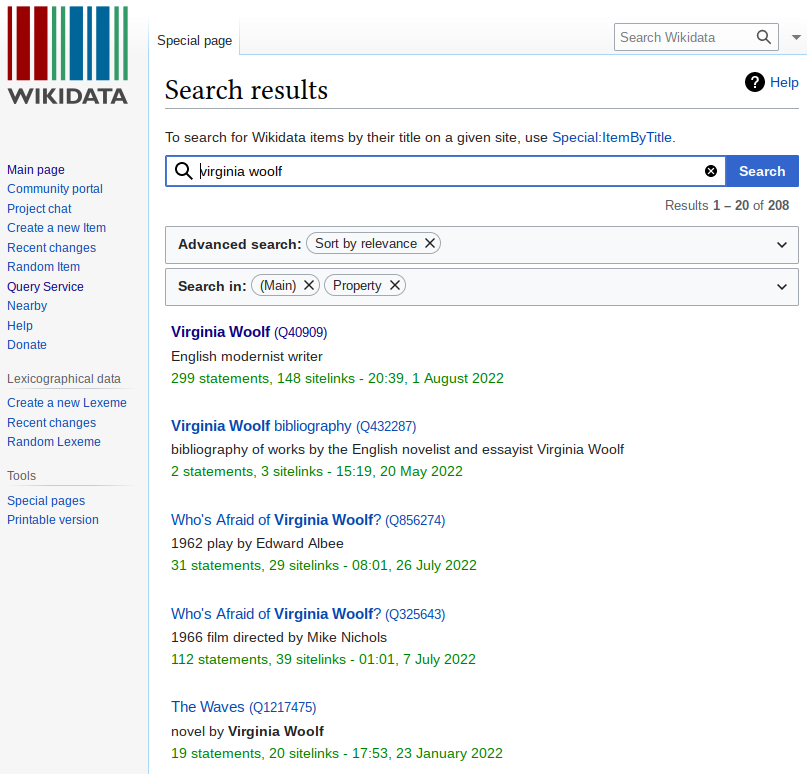
\includegraphics[width=\textwidth]{img/wd_base.png}
		\caption{Résultats retournés par le site traditionnel}
		\label{fig:wd_base}
	\end{subfigure}
	\begin{subfigure}{0.48\textwidth}
		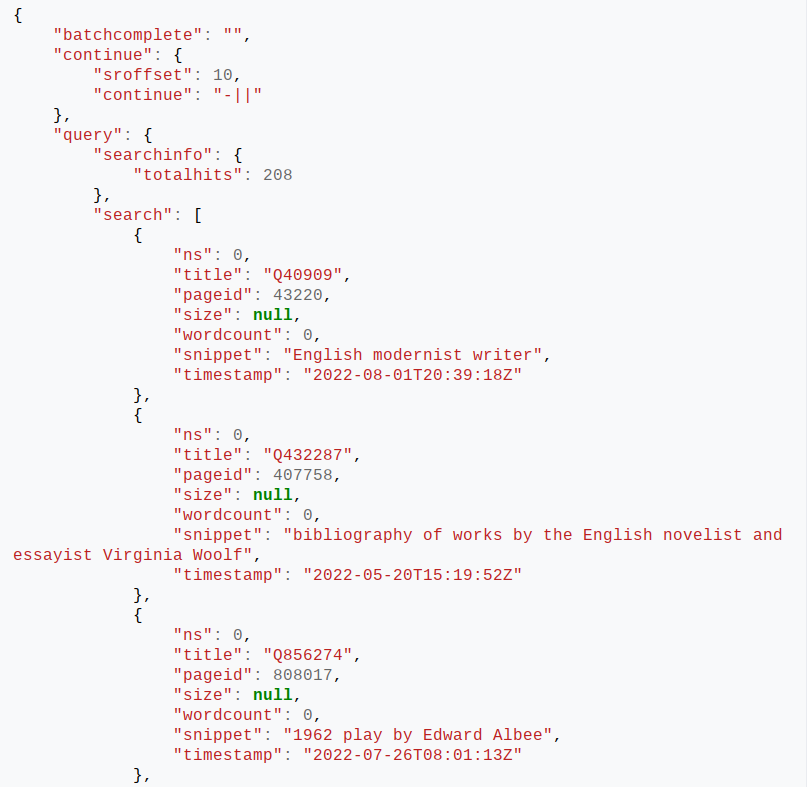
\includegraphics[width=\textwidth]{img/wd_api.png}
		\caption{Résultats retournés par l'\api{}}
		\label{fig:wd_api}
	\end{subfigure}
	\caption{Résultats retournés par \wkd{} pour la recherche \enquote{Virginia Woolf}}
	\label{fig:wd_search}
\end{figure}

Enfin, les données récupérées sont les mêmes, mais dans deux formats très différents (\ref{fig:wd_search}). Dans l'image de gauche (\ref{fig:wd_base}), les résultats sont visibles avec une interface graphique complète, comme sur n'importe quel site Web. À droite cependant (\ref{fig:wd_api}), les résultats sont présentés sous la forme de données structurées au format \json{} (format analogue à un \gls{dictionnaire}). Ce résultat contient à la fois les résultats à proprement parler (en dessous de \enquote{Search}) et des informations descriptives. Par exemple, \texttt{query/searchinfo/totalhits} retourne le nombre de résultats pertinents, soit 208 pages.

Cette brève présentation de la manière de consommer concrètement une \api{} indique également le protocole à suivre pour l'alignement des \tname{} avec des entités \wkd{}: il s'agit de concevoir un algorithme qui, à partir des données extraites du \tname{} et du \ttrait{}, construise des \gls{url} pour lancer des recherches en plein texte sur \wkd{}. Cela revient à associer au paramètre de l'\gls{url} \texttt{srsearch} la chaîne de caractère qui doit être recherchée sur la base de données de \wkd{}. Ensuite, l'algorithme doit transmettre à l'\api{} ces \url{}, interpréter le \json{} renvoyé par \wkd{} et enregistrer ces réponses dans un fichier. Étant donné que l'alignement avec \wkd{} prend plusieurs dizaines d'heures et demande des performances élevées, des \glspl{log} annexes sont créés en cours d'utilisation pour optimiser l'algorithme.


\subsection{Présentation générale}
L'algorithme d'alignement avec \wkd{} construit des \gls{url} et lance des recherches en plein texte sur l'\api{} \wkd{}. De par son fonctionnement, il multiplie les requêtes. Puisqu'il est impossible de vérifier en cours d'exécution si la réponse retournée par l'\api{} contient un résultat valide, il est nécessaire d'organiser l'algorithme afin de maximiser la probabilité d'obtenir un résultat valide. C'est pourquoi les recherches sont faites en commençant par les celles qui ont la plus grande certitude d'obtenir des résultats valides et en terminant par les plus incertaines. Dès qu'une réponse est obtenue, l'algorithme s'arrête et l'entrée de catalogue suivante est traitée. Comme cela apparaît dans la figure \ref{fig:apialgo}, il a par conséquent un fonctionnement à plusieurs étapes.

La première étape est la même quelles que soient les informations contenues dans le \tname{}: l'ensemble des paramètres\footnote{Dans ce qui suit, le terme \enquote{paramètre} se réfère aux clés du dictionnaire d'informations structurées, et non aux paramètres de l'\api{} présentées ci-dessus (\texttt{srsearch}...).} extraits lors de l'étape précédente sont mis bout à bout afin de lancer une recherche. Cela permet que la recherche soit la plus précise possible, afin de maximiser les possibilités d'obtenir un résultat valide.

Si la réponse de l'\api{} ne contient pas de résultat, alors les données disponibles sont étudiées afin d'adopter le bon comportement. Comme cela a été dit, différents processus ont été utilisés pour extraire des données du \tname{} et du \ttrait{}; il est donc logique de ne pas traiter tous les \glspl{dictionnaire} de données de la même manière.

Si l'entrée concerne une personne noble (c'est-à-dire, si le dictionnaire de données contient un nom de famille noble), alors il y a un possible conflit dans les données extraites: si le nom de famille usuel est recherché en même temps que le nom de famille noble sur \wkd{}, il arrive qu'aucun résultat ne soit retourné. Dans ce cas, une première requête est lancée en supprimant le nom de famille noble; si aucun résultat n'est obtenu, celui-ci est rajouté et c'est le nom de famille usuel qui est enlevé. Pour finir, une autre recherche est lancée sans le prénom. Si à ce stade aucun résultat n'a été obtenu, alors un algorithme de recherches soustractives est lancé; celui-ci est décrit plus bas.

Le deuxième cas de figure concerne la reconstitution des prénoms. Bien que celle-ci augmente la proportion de résultats valides, un prénom mal reconstitué risque de retourner du silence. C'est pourquoi une clé \texttt{rebuilt} a été ajoutée au \gls{dictionnaire} qui contient les données extraites: cette clé permet d'indiquer qu'un nom a été reconstitué. Dans ce cas, une nouvelle recherche est lancée sans le prénom. Si aucun résultat n'est obtenu, alors c'est l'algorithme de recherches soustractives qui s'exécute.

Le troisième cas de figure concerne la présence de plusieurs paramètres de recherche disponibles -- en langage technique, de plusieurs valeurs non-nulles dans le \gls{dictionnaire}. Dans ce cas, c'est directement l'algorithme soustractif qui s'exécute. Celui-ci a été conçu à partir du constat que, d'un côté, les données contiennent inévitablement de bruit; de l'autre, l'extraction de données risque elle aussi d'introduire du bruit. Cette logique soustractive cherche donc à supprimer le bruit qui a pu s'introduire. Afin d'éviter d'être trop \enquote{brut}, l'algorithme procède en séparant les différents types de bruit possibles. D'abord, il arrive souvent qu'un chiffre soit mal reconnu lors de l'océrisation, et il peut donc y avoir des erreurs dans les dates. Deux dates peuvent être extraites (naissance et décès); il y a cependant peu de chances d'erreur sur les deux dates. Par conséquent, une des deux dates est supprimée et la recherche est lancée; si aucun résultat n'est obtenu, c'est l'autre date qui est supprimée. La seconde source de bruit provient des prénoms: comme cela a été dit, au \scl{XIX}, les prénoms étrangers sont régulièrement traduits; il arrive souvent que les prénoms composés ne soient pas dans le même ordre que sur \wkd{}, ou qu'une personne soit nommée par son deuxième prénom -- peut-être parce que les catalogues utilisent des noms d'usage alors que \wkd{} s'en tient aux noms civils. Pour ces raisons, le prénom est retiré de la chaîne de caractères à rechercher avant de faire une requête sur l'\api{}. Bien que les risques liés aux dates et aux prénoms ont été corrigés (autant que possible), il est possible que l'auteur.ice n'ait pas encore été aligné avec une entité \wkd{}. À ce stade, tous les risques spécifiques ont été traités. L'algorithme relance alors des recherches en retirant à chaque fois un paramètre différent, jusqu'à ce qu'un identifiant ait été extrait de \wkd{} ou que toutes les permutations possibles aient été faites.

Cette série de construction d'\gls{url} cherche à minimiser les redondances; cependant, il est possible qu'une même chaîne de caractères puisse être extraite à différentes étapes. C'est pourquoi des \glspl{log} sont créés en cours d'utilisation: ils servent à sauvegarder les chaînes de caractères qui ont déjà été recherchées et les résultats qui leur sont associées. Avant de lancer une requête sur l'\api{}, l'algorithme vérifie donc si la chaîne a déjà été recherchée. Si oui, il récupère le résultat obtenu; sinon, lance la recherche et sauvegarde le résultat retourné par \wkd{}.

L'algorithme de recherche sur \wkd{} est visiblement complexe, puisque son objectif est de minimiser le taux d'erreur possible sur des données variées, ce qui demande d'adopter des comportements différents en fonction des informations disponibles. L'algorithme ayant tendance à retirer de plus en plus de paramètres de recherches en cours d'exécution (les dates, les prénoms...), il est possible que la chaîne recherchée finisse par être très pauvre en informations; cela permet de s'aligner avec une entité, mais celle-ci risque de ne pas correspondre au \tname{} ou d'être très générique. Si l'entité recherchée est \enquote{Napoléon Bonaparte}, mais que suffisamment de paramètres ont été retirés, il est possible que l'algorithme ne recherche que \enquote{Bonaparte}. Le résultat obtenu est alors \href{https://www.wikidata.org/w/index.php?search=bonaparte&search=bonaparte&title=Special%3ASearch&go=Go&ns0=1&ns120=1}{\enquote{Charles Lucien Bonaparte}}. Il est donc utile d'avoir une mesure de la certitude (ou l'incertitude) de la validité d'un résultat, ne serait-ce que pour accélérer le processus de correction des identifiants (ce qui, sur plus de 82000 entrées, n'est pas une mince affaire). Le parti pris a été, tout simplement, d'établir un score de certitude en fonction du nombre de paramètres utilisés pour lancer une recherche. Ce score a été défini de façon expérimentale, en mesurant la proportion de résultats considérés comme certains et ainsi que le taux d'erreur au sein des résultats certains (c'est-à-dire, le nombre de résultats qui ont dépassé le seuil de certitude mais qui sont en fait erronés). Après plusieurs essais différents, le score de certitude \(c_r\) pour un résultat \(r\) a été déterminé. Il suit la formule ci dessous:

\begin{align*}
	\text{Étant donnés:} \\ 
	&c_r \text{ le score de certitude pour un résultat } r \text{;}\\
	&q_r \text{ la chaîne de caractère recherchée pour obtenir le résultat } r \text{;}\\
	&\sum param \text{ la somme des paramètres utilisés dans } q_r \text{;} \\
	&d = 1 \text{ si une date est dans } q_r \text{ ; sinon, } d = 0 \text{;} \\
	&p = 1 \text{ si le prénom utilisé dans } q_r \text{ n'a pas été reconstitué; sinon, } p = 0 \text{;}
\end{align*}
\begin{displaymath}
	c_r = \sum param + d + p
\end{displaymath}

\bigskip
Un résultat est considéré comme étant \enquote{certain} si \(c_{r} >= 4\) ou si des dates sont présentes dans \(q_r\) (les chances qu'un alignement soit fait entre un \tname{} et une entité homonyme ayant les mêmes dates de naissance ou de décès étant très faibles). Sur le jeu de données de test, 32\% des entrées atteignent ce seuil de certitude. 23,6\% de celles-ci comprennent en fait une erreur, soit 8,5\% du jeu de données total (voir le tableau en annexes: \ref{appendix:testfinal}). L'objectif de ce score de certitude n'est pas d'être parfaitement exact, mais d'accélérer la relecture des résultats: en acceptant un taux d'erreur total de 8,5\%, il est possible ne corriger que les entrées pour lesquelles \(c_r < 4\). Seuls les deux tiers du jeu de données restent alors à corriger manuellement.

Cet algorithme cherche à répondre à plusieurs problèmes techniques: il travaille avec des données historiques contenant du bruit et un niveau très inégal d'information. Son fonctionnement vise à maximiser la probabilité d'obtenir un résultat valide, en faisant des requêtes d'abord très spécifiques puis de plus en plus génériques. Cependant, il crée lui-même plusieurs problèmes: son fonctionnement est assez complexe et demande de manipuler plusieurs lourds fichiers en même temps. Un ensemble d'optimisations ont donc été réalisées.

\widepage
\begin{figure}[!p]
	\centering
	\tikz[scale=0.70, transform shape]{
		\node[base] (start) at (-8,8)%
			{Dictionnaire structuré contenant les données à rechercher sur l'\api{}};
		\node[transf] (firsturl) at (0,8)%
			{\textbf{Préparation de la première requête} \\ Premier URL mettant bout à bout tous les paramètres disponibles};
		\node[choice] (type) at (0,1.5)%
			{\textbf{Préparation de la deuxième série de requêtes} \\ Quel type d'entrée est-ce? Quelle données sont disponibles?};
					
		\node[base] (many) at (0,-4)%
			{Plusieurs paramètres de recherche sont disponibles};
		\node[base] (rebuilt) at (8,-4)%
			{Le prénom est reconstitué};
		\node[transf] (rebuilttr) at (8,-9)%
			{Constitution d'un nouvel URL sans le prénom};
		\node[transf] (sub) at (0,-9)%
			{Algorithme soustractif *};
		\node[base] (noble) at (-8,-4)%
			{C'est le nom d'une personne noble};
		\node[transf] (nobletr) at (-8,-9)
			{
				Préparation d'URLS par retrait successif des 
				différentes informations nominatives:
				\begin{itemize}
					\item Prénom
					\item Nom de famille usuel
					\item Nom de famille noble
				\end{itemize}
			};

			
		\node[transf] (launch) at (0,-15)%
			{Lancement de la requête};
		\node[db] (log) at (8,-18)%
			{Fichiers de log};
		\node[transf] (cert) at (0,-20)
			{Évaluation de la certitude du résultat};
		\node[db] (end) at (0,-23)%
			{Enregistrement des résultats};
			
		\node[blank] at (7,-15.3) {Si la première requête ne retourne pas de résultat};
		\node[blank,rotate=-90,text width=3.8cm] at (2.6,-11.8) {Si les deuxièmes séries de requêtes ne retournent pas de résultat};
		\node[blank,text width=4cm] at (4,-16.7) {Vérifier si la requête a déjà été lancée};
		\node[blank,text width=4cm] at (4,-18.6) {\begin{flushright}Enregistrer la requête si elle est lancée\end{flushright}};
		\node[outline, text width=7cm] (note) at (8,7)%
			{
				*: L'algorithme soustractif consiste à:
				\begin{itemize}
					\item si il y a deux dates (naissance et décès), en supprimer une des deux et relancer la requête
					\item si il y a plusieurs paramètres, retirer tous les paramètres un à un et relancer la requête
					\item pour finir, si encore aucun résultat n'a été obtenu, supprimer le prénom et relancer la requête
				\end{itemize}
			};
		\node[blank,text width=3cm,rotate=90] at (-1,-17.25) {Si un identifiant est trouvé, le script s'arrête};
		
			
		\begin{pgfonlayer}{bg}
			\draw[arrow] (start) -- (firsturl);
			\draw[arrow] (firsturl) -- (0,5) -- (-12.5,5) -- (-12.5,-15) -- (launch);
			\draw[arrow] (launch) -- (12.5,-15) -- (12.5,1.5) -- (type);
			\draw[arrow] (type) -- (noble);
			\draw[arrow] (type) -- (rebuilt);
			\draw[arrow] (type) -- (many);
			\draw[arrow] (noble) -- (nobletr);
			\draw[arrow] (many) -- (sub);
			\draw[arrow] (rebuilt) -- (rebuilttr);
			\draw[arrow] (nobletr) -- (-8,-14.5) -- (-2.5,-14.5) -- (launch);
			\draw[arrow] (rebuilttr) -- (8,-14.5) -- (2.5,-14.5) -- (launch);
			\draw[arrow] (sub) -- (launch);
			\draw[arrow] (launch) -- (1.5,-14.5) -- (1.5,-9.75) -- (sub);
			\draw[arrow] (launch) -- (cert);
			\draw[arrow] (cert) -- (end);
			\draw[arrow] (launch) -- (1.5,-15.5) -- (1.5,-17.25) -- (5.5,-17.25) -- (log);
			\draw[arrow] (launch) -- (1.5,-15.5) -- (1.5,-18.25) -- (5.5,-18.25) -- (log);
		\end{pgfonlayer}	
		
	}
	\caption{Algorithme lançant des recherches en plein texte sur \wkd{}}
	\label{fig:apialgo}
\end{figure}
\restoregeometry

\subsection{Gérer la montée en charge: optimisation et réduction du temps d'exécution}
L'intégralité de l'algorithme (contenant extraction d'informations et interaction avec une \api{}) a cessé de fonctionner sur mon ordinateur alors qu'à peine 5\% des 820000 entrées avaient été traitées. Ce problème technique soulève des difficultés adjacentes à la recherche en humanités numériques: dans ce contexte, des ordintateurs très performants ne sont pas toujours disponibles, et les machines utilisées sont souvent des ordinateurs de bureau traditionnels. De telles situations, la recherche peut parfois faire face à des limitations matérielles. De telles limites sont -- bien sûr -- un problème; en obligeant chercheur.euse.s à intégrer des contraintes matérielles dans leurs algorithmes, cette difficulté peut aider à réaliser des programmes plus efficaces, moins gourmands en ressources et en énergie, et donc aider à faire de la recherche plus durable. De telles considérations écologiques sont partagées par toute une communauté de chercheur.euse.s issu.e.s des humanités et défendant des approches \enquote{low-tech}\footnote{
	Le \textit{Minimal computing} (\enquote{Informatique minimale} en français) est un groupe de réflexion créé au sein de \textit{GO::DH -- Global Outlook Digital Humanities}. Il s'intéresse aux manières de rendre l'informatique minimale, dans différents sens du terme: à la fois plus accessible, mais également plus écologique. Plus généralement, le courant du \textit{minimal computing} développe une approche réflexive sur les façon de faire de la recherche durable et libre (au sens de l'\gls{open source}); ce groupe s'intéresse également au développement des humanités numériques dans un contexte non-occidental\cite{sayers_minimal_2016}.
}; ces considérations écologiques sortent du champ des humanités et se retrouvent dans des travaux provenant de l'informatique \enquote{traditionnelle} et de l'apprentissage machine\footcite{strubell_energy_2019}. L'optimisation de programmes informatique n'est pas seulement une question écologique: c'est également une manière d'écrire de meilleurs programmes, plus performants et efficaces.

Dans sa première version, le script d'alignement avec \wkd{} avait un fonctionnement apparemment plus \enquote{simple}, puisqu'il ne prenait pas du tout en compte les questions d'optimisation: pour chaque entrée de catalogue, des informations étaient extraites et les recherches faites sur \wkd{}. Ce fonctionnement avait deux défauts. D'abord, il demandait que tout le script soit exécuté en une fois -- si il y a une erreur imprévue, il est nécessaire de recommencer à nouveau. Ensuite, une interaction avec \wkd{} était nécessaire pour chaque entrée, peu importe si le nom contenu dans le \tname{} avait déjà été recherché auparant (alors qu'une même personne est souvent l'auteur.ice de plusieurs manuscrits recensés dans les catalogues); l'interaction avec \wkd{} prenant plusieurs secondes, cela peut grandement ralentir le processus d'alignement avec \wkd{}. C'est à partir de ces deux problèmes que le processus d'optimisation a commencé.

Le premier problème -- l'impossibilité de vérifier quelles entrées de catalogue ont déjà été traitées -- a d'abord été corrigé en consultant, à chaque fois qu'un nouvel identifiant était recherché, le fichier de sortie. Celui-ci est un tableur qui contient l'identifiant des entrées, le \tname{}, le \ttrait{}, l'identifiant récupéré sur \wkd{} et un extrait de la description associée à cet identifiant. Si cette solution permet de ne pas recommencer à zéro à chaque fois que le script est lancé, elle demande de charger en mémoire un très large fichier \texttt{csv} (12,7 mégaoctets). Cette vérification particulièrement gourmande a été remplacée par la création d'un \gls{log} annexe en cours d'exécution. Celui-ci contient uniquement les identifiants des différentes entrées de catalogue et mesure seulement 1,3 mégaoctets. À chaque fois qu'une nouvelle entrée est traitée, ce fichier est ouvert, et le script vérifie que le nouvel identifiant ne s'y trouve pas. Si l'identifiant ne s'y trouve pas, alors le \tname{} et le \ttrait{} de cette entrée sont traités et alignés avec un identifiant \wkd{}. À la fin de ce processus, l'identifiant \tei{} de l'entrée est ajouté au \gls{log}. Cette simple modification permet donc de vérifier si une entrée de catalogue a déjà été traitée à l'aide d'un fichier dix fois moins lourd que dans la tentative précédente.

Ce processus permet de vérifier quelles entrées ont déjà été traitées, mais il ne permet pas de savoir si une personne se retrouve d'une entrée sur l'autre. Si une telle récurrence est identifiée, il serait possible de récupérer les résultats déjà disponibles, plutôt que de réaliser à nouveau l'alignement avec \wkd{}. Non seulement cela pourrait rendre le script plus rapide -- le lancement des requêtes pour une entrée prenant environ 2 à 5 secondes --, mais en plus, cela éviterait de surcharger l'\api{} de requêtes, ce qui, dans un cas extrême, peut faire saturer une application en ligne et perturber son fonctionnement. La difficulté consiste alors à désambiguïser les informations présentes dans le \tname{} (c'est-à-dire, à repérer toutes les occurrences d'une même personne dans les \tname{}). Cette désambiguïsation est compliquée (l'un des intérêts de la reconnaissance d'entités nommées est justement d'identifier les multiples occurrences d'une même personne). Plutôt que de trouver un moyen de désambiguïser réellement les entrées, une solution plus simple a été mise en place: chaque chaîne de caractère recherchée est enregistrée dans un \gls{log}, avec l'identifiant \wkd{} récupéré par recherche. L'intégralité du processus d'extraction d'information des \tname{} et \ttrait{} est donc menée sur toutes les entrées; toutes les chaînes de caractères à rechercher sont également construites; cependant, une recherche n'est faite sur l'\api{} que si elle n'a jamais été faite auparant. Du fait de la taille du jeu de données, un problème apparaît cependant: plusieurs chaînes de caractères étant construites pour chaque entrée de catalogue, l'utilisation d'un seul \gls{log} pour contenir toutes ces recherches amènerait à la création d'un immense fichier (plusieurs centaines de milliers de lignes). Il serait alors nécessaire de le parcourir intégralement à chaque fois qu'une requête est lancée; le script optimisé risquerait alors d'être moins efficace qu'avant son optimisation. Le choix a donc été fait de créer automatiquement et d'utiliser plusieurs \glspl{log}: les chaînes de caractères y sont enregistrées en fonction du premier caractère qu'elles contiennent, avec un \gls{log} par lettre. Ainsi, avant de lancer une recherche, le fichier à parcourir est bien plus court (2060 entrées pour la lettre \enquote{e}).

Avec toutes ces optimisations, le script a pu fonctionner en utilisant au maximum 3 gigaoctets, soit l'équivalent de naviguer sur internet en ayant un logiciel de traitement de texte ouvert (sur ma machine). Cependant, l'utilisation \glspl{log} faite ici -- qui a elle même été optimisée -- demande de faire un arbitrage. En n'enregistrant pas de données et en lançant des requêtes à chaque fois, c'est la charge processeur qui augmente, ainsi que la consommation de courant due à internet. En enregistrant les requêtes déjà lancées, ces charges là sont diminuées, mais l'utilisation de mémoire vive augmente (il faut charger en mémoire et lire de larges fichiers). De ces deux deux différentes approches (augmenter la charge processeur ou augmenter la mémoire vive) il est nécessaire de déterminer laquelle est la plus efficace. C'est un des objectifs des tests menés sur l'algorithme d'alignement avec des identifiants \wkd{}, comme nous allons le voir maintenant.

\subsection{Évaluer du script : performance, qualité des données extraites de \wkd{} et comparaison avec d'autres projets}
Le processus d'alignement avec des entités \wkd{} n'est pas parfait, et implique nécessairement un taux d'erreur. Au vu de la taille du corpus, la correction des résultats est un processus particulièrement chronophage. Pour pouvoir utiliser les données produites avant cette correction, il est nécessaire de trouver une manière d'évaluer la qualité des résultats. Des tests ont été réalisés pour faire cette évaluation. Ils ont également été utilisés durant tout le développement de ce processus, afin de comparer les différents algorithmes d'extraction et de requêtes entre eux. Les tests ont également permis de mesurer l'impact de chaque paramètre de recherche dans l'obtention d'un résultat valide. Enfin, l'évaluation des algorithmes permet de comparer sa version optimisée et non-optimisée.

Comme cela a déjà été dit, les tests ont été lancés sur un jeu de données représentatif contenant 200 \tname{} et \ttrait{}, choisis dans différents catalogues; ce jeu de test représentant également les différents types de noms possibles (de personnes nobles, de lieux...); enfin, la proportion de \ttrait{} dans le jeu de données complet et dans celui de test est la même. Deux catégories de tests ont été réalisés. Le premier, décrit plus haut, concerne l'impact de chaque paramètre dans l'obtention d'une entité correcte sur \wkd{} (\ref{appendix:testisolate}). Le second sert à mieux identifier les performances de l'algorithme final (\ref{appendix:testfinal}). 

Ce dernier test réalise l'intégralité du processus d'extraction d'informations et d'alignement avec \wkd{} sur l'ensemble du jeu de test. Ce processus est réalisé trois fois sans utiliser des \glspl{log} et trois fois en les utilisant (c'est-à-dire, en inscrivant les recherches déjà faites dans un fichier et en vérifiant avant chaque recherche si une chaîne de caractère a déjà été recherchée). Faire plusieurs fois de suite le même processus permet de les variations de performance induites par l'utilisation de \glspl{log}. La performance d'un script, en terme d'utilisation des processeurs et de la mémoire vive, est assez difficile à quantifier; elle peut également varier d'une machine à une autre; enfin, il n'est pas possible de mesurer la charge supplémentaire infligée à un serveur distant lors de l'utilisation répétée de sources de données en ligne. Le seul critère retenu a donc été le temps d'exécution. Le script étant lancé trois fois en utilisant des \glspl{log} et trois fois sans, les deux temps d'exécution \(\bar{t}\) correspondent au temps moyen nécessaire à traiter les 200 entrées du jeu de test. Soit \(t_i\) le temps pris pour traiter une fois le jeu de test, la moyenne \(\bar{t}\) correspond à:

\begin{displaymath}
	\bar{t} = \frac{1}{3}\sum_{i=1}^{3}t_i
\end{displaymath}

La difficulté pour mesurer les temps d'exécution \(t_i\) en utilisant des \glspl{log} est que, en dehors des tests, ces fichiers sont de plus en plus volumineux; le temps utilisé pour les parcourir augmente en conséquence. Pour que ces \(t_i\) soient représentatifs, de faux \glspl{log} sont créés avant le lancement des tests: ceux-ci comprennent des fausses données qui correspondent environ aux résultats obtenus pour 30000 recherches lancées sur l'\api{} (soit un peu moins que les 82000 entrées du jeu complet, en prenant en compte que certaines recherches ne retournent pas de résultat, ce qui allège d'autant le fichier à parcourir). Le temps d'exécution \(\bar{t}\) en utilisant des \glspl{log} est de 88,3 secondes; sans ces fichiers, \(\bar{t}\) est de 92,5 secondes. Si la différence entre les deux résultats n'est pas immense, l'utilisation de \glspl{log} permet également la charge processeur et l'interaction avec \wkd{}, ce permet d'autres améliorations au delà du seul temps de performance.

À part cette seule évaluation de performance, les tests sur l'algorithme final (\ref{appendix:testfinal}) servent à mesurer la qualité des résultats obtenus. La mesure de performance pour un processus d'alignement est le \gls{score F1}, qui prend à la fois en compte la précision (le nombre de vrais positifs obtenus parmi tous les résultats obtenus) et le rappel (le nombre de vrais positifs obtenus parmi tous les vrais positifs). Celui-ci est de 67,4\%, ce qui marque une nette amélioration (près de 20 points) de l'utilisation seule du prénom et du nom de famille usuel extrait du \tname{}. 

Ce score est également intéressant en comparaison avec d'autres projets de \gls{nel}, sous-domaine du traitement automatisé du langage qui vise à associer une entité avec une base de connaissances externes. Aicha Soudani et al. ont, en 2018, présenté les résultats d'un projet de \gls{nel} de lieux sur un corpus relativement proche du notre: des textes littéraires du \scl{XIX} encodés en \xmltei{}. \footcite{soudani_adaptation_2018}. Les méthodes utilisées par ce projet diffèrent largement de celles présentées ici: les auteur.ice.s s'appuient fortement sur l'apprentissage machine, en identifiant d'abord des entités dans le texte à l'aide de \texttt{SEM} avant de lier les entités à différentes bases de connaissance en utilisant \texttt{REDEN}. Leur projet présente donc une complexité supplémentaire, puisqu'il demande de repérer les entités, ce qui n'est pas le cas ici (elles se trouvent toutes dans des balises \tname{}). Cependant, c'est cette deuxième étape qui nous intéresse; les entités ont déjà été identifiées, ce qui nivelle cette différence entre les projets. Trois bases de données en ligne ont été utilisées: \textit{DBPedia}, \textit{DataBNF} et \wkd{}. En comparaison avec ce projet, il est intéressant de remarquer que le processus d'alignement avec \wkd{} développé par \mssktb{} obtient un \gls{score F1} très satisfaisant (67,4\%). Celui-ci dépasse les scores obtenus par Soudani et al. dans leur alignement avec \wkd{} (61,1\%) et \textit{DBPedia} (53,6\%)\ (voir le détail des résultats en annexe: \ref{appendix:soudani}). Les résultats comparativement faibles de Soudani et al. s'expliquent en partie par le fait que \texttt{REDEN} recherche des candidats pour le liage d'entités en établissant une correspondance parfaite des caractères (\textit{exact string match})\footcite[p. 4]{soudani_adaptation_2018}\footnote{Il est également à remarquer que Soudani et al. disposent d'un score d'\enquote{exactitude totale du liage} (\textit{Overall linking accuracy}) qui est nettement plus élevé (entre 70 et 85\%); la méthode de calcul de ce score, qui mesure la performance de l'ensemble du processus de \gls{nel}, n'est cependant pas décrite dans l'article. Il est donc impossible d'y comparer les résultats de \mssktb{}.}. Les scores comparativement positifs du projet \mssktb{} sont peut être également rendus possibles par la quantités d'informations disponibles sur chaque personne dans le corpus, récupérée grâce à un travail d'extraction des données sur l'ensemble du \ttrait{} et du \tname{}.

\subsection{Conclusion: retour sur l'extraction d'informations des catalogues et sur l'algorithme d'alignement avec \wkd{}}
L'algorithme liant les noms d'auteur.ice dans les catalogues avec des entités \wkd{} propose une réponse à plusieurs difficultés techniques propres à la reconnaissance d'entités par la détection de motifs sur un corpus de données varié. Parmi toutes ces difficultés possibles, les trois les plus importantes sont le bruit dans les données d'origine, le bruit produit par l'extraction de données et enfin la difficulté à réaliser un alignement entre des documents historiques et des bases de données contemporaines. La solution proposée s'appuie sur un fonctionnement modulaire, qui s'adapte aux données produites et prend en compte la possibilité que du bruit se soit introduit à une étape ou à une autre. De différence de résultats obtenue avec Soudani et al., il faut retenir que la technique utilisée n'est pas toujours garante de la qualité des résultats obtenus. Plutôt que de chercher à établir des correspondances exactes, l'approche décrite dans ce mémoire, basée sur une détection de motifs \textit{low-tech} a permis de développer une méthode très précisément adaptée à la fois au corpus et à \wkd{}. Ce qui est potentiellement perdu par la détection de motifs est donc corrigé par l'algorithme menant des requêtes sur \wkd{}. 

L'alignement avec des entités \wkd{} est la meilleure manière de corriger le bruit dans les données du projet: en liant les différents \tname{} à des identifiants \wkd{}, il devient possible d'extraire des données structurées d'une source externe, pour construire une base de connaissance plus fiable: même si un corpus semi-structuré facilite le travail d'extraction d'informations, l'accès aux informations reste relativement complexe; il existe de plus des biais dans les informations contenue par le corpus (ce qui est mis en avant dans les \ttrait{} est avant tout ce qui est susceptible d'intéresser le public de l'époque). En se servant de ce liage d'entités pour constituer une base de données, il est possible de chercher à corriger ce biais dans les données, tout en rassemblant assez d'informations pour pouvoir faire une analyse des facteurs déterminant le prix d'un manuscrit sur le marché du  \scl{XIX}. C'est la manière dont est constitué le jeu de données issu de \wkd{} qui est expliqué ci-dessous.

\section{Après l'alignement, l'enrichissement: utiliser \sparql{} pour produire des données structurées}
Le liage des noms contenus dans le \tname{} avec \wkd{} n'est qu'une étape, et non la fin en soit du processus -- bien que ce soit la partie la plus difficile. Les identifiants ainsi récupérés servent de \enquote{porte d'entrée} aux données disponibles sur la base de connaissance: une fois que ces identifiants sont connus, il est possible de récupérer automatiquement via \sparql{} des données sur les auteur.ice.s et autres entités présentes dans les catalogues. Obtenir ces informations permet avant tout de mieux situer l'auteur.ice d'un manuscrit, afin mieux le statut d'une personne et de comprendre quelles informations biographiques influencent le prix d'un manuscrit. Mais le liage d'entités nommées peut avoir d'autres fins et permettre d'enrichir le corpus de catalogues de plusieurs manières, comme nous le verrons.

\subsection{Comprendre les particularités des modèles sémantiques de données}
Un bref retour sur la manière dont s'organisent les données contenues dans \wkd{} permet de mieux comprendre le problème que peut poser la diversité du corpus pour la constitution d'une base de connaissances propre au projet. \wkd{}, comme de nombreuses autres bases en lignes (\textit{DataBNF, DBPedia...}), permet d'accéder à des informations stockées dans une \gls{graph}. Ce type de base de données a un fonctionnement très particulier qui influence la constitution d'une base de connaissance à partir des identifiants \wkd{} récupérés à l'étape précédente. Dans une \gls{graph}, les données sont encodées en \xml{}-\rdf{}. Ce format -- dit sémantique -- contient des données liées sous forme de \enquote{triplets} sujet--prédicat--objet, où:

\begin{itemize}
	\item le sujet est la ressource principale.
	\item le prédicat est une propriété du sujet, qui caractérise une relation avec une autre ressource, l'objet.
	\item l'objet est une ressource secondaire: c'est la valeur d'un prédicat.
\end{itemize}

Le principe des triplets \rdf{} est mieux exprimé sous forme graphique (\ref{fig:triplet}):

\begin{figure}[!h]
	\centering
	\tikz{
		\node%
		[base] %
		(S) at (0,0) %
		{\textbf{Sujet} \small \\ La ressource principale \\ \textit{Natalia Gontcharova}};
		\node%
		[transf] %
		(P) at (5, 0) %
		{\textbf{Prédicat} \small \\ La relation à l'objet \\ \textit{a peint}};
		\node%
		[base] %
		(O) at (10, 0) %
		{\textbf{Objet} \small \\ Une ressource secondaire \\ \enquote{\textit{Les porteuses}}};
		
		\draw[arrow] (S) -- (P);
		\draw[arrow] (P) -- (O);
	}
	\caption{Exemple de relation sujet -- prédicat -- object}
	\label{fig:triplet}
\end{figure}

Trois particularités supplémentaires définissent les formats sémantiques:
\begin{itemize}
	\item Toutes les \enquote{ressources} peuvent être tour à tour sujet ou objet. L'exemple du dessus, par exemple, aurait pu être réécrit sous la forme: \enquote{Les porteuses} a été peint par Natalia Gontcharova. Dans ce cas, Natalia Gontcharova est l'objet et \textit{Les porteuses} est le sujet. Par conséquent, une base de données \rdf{} est une \gls{graph}; elle peut être représentée sous la forme d'un réseau de ressources qui entretiennent des relations bilatérales entre elles. Il n'y a pas de hiérarchie entre les informations, contrairement à une base de données \xml{} classique.
	\item L'ensemble des ressources et des prédicats d'une \gls{graph} sont définis et disposent d'un identifiant unique (certains de ces identifiants ont été récupérés grâce au liage d'entités nommées).
	\item Si le langage \sparql{} offre une syntaxe commune, chaque base de connaissance peut utiliser des vocabulaires particuliers qui sont organisés en \enquote{ontologies}. Une ontologie correspond à la définition d'un ensemble de catégories, de propriétés et de relations qui unissent des données et des concepts; cet ensemble est complété par une modélisation (souvent sous forme graphique), qui indique la relation entre les différents termes de l'ontologie\footcite{noauthor_ontology_2022}. Ceux-ci sont souvent liés de façon hiérarchique (plusieurs termes spécifiques pouvant être dérivés d'un terme générique). Au sein d'une ontologie, chaque terme a lui-même un identifiant unique, ce qui garantit une implémentation uniforme pour l'ontologie. Une même base de connaissance peut utiliser plusieurs ontologies. Celles-ci sont définies à l'aide d'espaces de noms\footcite{noauthor_namespace_2022}, c'est-à-dire par des identifiants qui permettent de différencier les ontologies. Les prédicats, plus particulièrement, sont définis selon une ontologie particulière.
\end{itemize}

\sparql{} a l'avantage de permettre de récupérer des données propres sur des bases en ligne et offre une syntaxe unique partout où il est implémenté. Cependant, le troisième point complexifie son utilisation, ainsi que la définition des données à récupérer: les prédicats sont décrits avec une grande précision et selon des vocabulaires spécifiques; par conséquent, une information analogue peut être représentée par différents prédicats selon le type de donnée qui est requêtée (une personne, une sculpture...). Dans l'ontologie \wkd{}, la création d'un texte et la création d'une peinture ne correspondent pas au même prédicat. Pour que les données soient utilisables, il faut être très spécifique quant aux informations recherchées. 

\subsection{Quelles données rechercher via \sparql?}
La question des données qui doivent être récupérées, et donc de la base de connaissance à constituer pour le projet \mssktb{} n'est pas anodine. D'abord, l'utilisation de sources externes peut être utiliser pour corriger des biais dans les données originelles (où ce sont les auteur.ice, éditeurs et éditrices de catalogues qui décident des informations à intégrer). Ensuite, si l'objectif premier est de récupérer des données pour mener une étude économétrique, le liage avec \wkd{} peut également permettre d'autres enrichissements et fonctionnalités. Enfin, cette étape représente une difficulté technique: le corpus de catalogues et les entités récupérées sont très diverses, tandis que \sparql{} utilise au contraire des vocabulaires très spécifiques. Il faut donc construire des requêtes très étendues, afin d'obtenir des résultats pour tous les types de données. Les 18899 entités avec lesquelles les entrées de manuscrits ont été alignées peuvent se classer en de nombreuses catégories. Sur \wkd{}, une entité est une \enquote{instance} d'une classe plus large. C'est en fonction de ces classes qu'il faut construire les requêtes: les propriétés recherchées pour chaque entité peuvent être spécifiques à une classe, mais pas à l'entité elle-même. En suivant la classification de \wkd{}, les entités présentes dans le corpus appartiennent aux catégories suivantes:

\begin{itemize}
	\item personnes humaines; cette catégorie est la plus fréquente (12090 occurrences)
	\item noms de familles (3180 entités)
	\item communes françaises (586 occurrences)
	\item peintures et sculptures (respectivement 520 et 236 entités)
\end{itemize}

Cette variété -- présentée sous forme graphique en annexes (\ref{appendix:wikidata_instances}) -- peut s'expliquer en partie par le taux d'erreur dans l'alignement avec \wkd{}: il est par exemple probable que les peintures et sculptures soient sur-représentées parmi les entités \wkd{} liées aux catalogues. Cependant, toutes ces \enquote{erreurs} ne correspondent pas forcément à des résultats qui ne sont pas pertinents. Par exemple, l'algorithme peut aligner un.e écrivain.e avec un de ses ouvrages, ou une personne avec son portrait. Des résultats erronés peuvent toujours garder une forme de pertinence. Il est d'autant plus important de construire des requêtes \sparql{} qui se concentrent pas uniquement sur des personnes. Cependant, il n'est pas possible de s'adapter à l'intégralité de la diversité du corpus. Le choix a donc été fait de se concentrer sur les catégories les plus pertinentes: les personnes, les familles, et les œuvres artistiques et littéraires. Non seulement ces catégories contiennent la grande majorité du corpus (16026 entités, soit 84,79\%), mais ces catégories sont les plus à même de contenir des entités pertinentes. Il a été choisi de ne pas faire de requête spécifique sur les lieux, puisque \wkd{} présente peu d'informations pour les entités de la catégorie \enquote{communes françaises}.

Un nombre assez conséquent de données ont donc été requêtées avec \sparql{}, du fait des spécificités des bases de données en graphes, de la variété des entités \wkd{} auxquelles les manuscrits sont liées, et enfin du fait de la variété du corpus lui même. Ces informations récupérées correspondent aux différentes catégories de \wkd{}.
\begin{itemize}
	\item Pour les personnes et les familles, les informations suivantes sont récupérées sur \wkd{}:
	\begin{itemize}
		\item Le genre de la personne;
		\item Sa nationalité, afin de voir si l'origine d'une personne influence le prix d'un manuscrit;
		\item Les langues parlées par une personne; là encore, l'objectif est d'étudier l'impact de l'origine d'un.e auteur.ice sur un prix.
		\item Les date de naissance et de décès, afin de placer un manuscrit dans une époque et de voir comment son ancienneté ou sa contemporanéité en influencent le prix.
		\item Le lieu où une personne est née, où elle a vécu et où elle est morte, pour des raisons analogues.
		\item La manière dont la personne est morte. Si cette information peut sembler anecdotique à un public contemporain, les catalogues de ventes sont marqués par un goût du sensationnel, et la manière dont une personne est morte est souvent mentionnée, notamment en cas d'exécutions.
		\item La religion d'une personne: il peut être intéressant d'étudier si, et comment, ce critère influence l'évolution d'un prix.
		\item Les titres de noblesse d'une personne.
		\item L'éducation qu'a reçu une personne, afin de mieux situer ses occupations et d'analyser l'impact du niveau et du type d'éducation sur le prix.
		\item L'occupation d'une personne, et les fonctions précises qu'elle a occupées: là encore, il est intéressant de situer l'impact de la carrière sur le prix et de voir quelles occupations sont corrélées avec des prix élevés sur le marché des manuscrits.
		\item Les prix et distinctions reçus par une personne. À l'aide de ce critère, il est alors possible de chercher à répondre à cette question: la célébrité d'une personne de son vivant impacte-elle le prix de se manuscrits?
		\item Les organisations et institutions dont la personne est membre (Académie française, Franc-maçonnerie...)
		\item Le nombre d'œuvres écrites ou réalisées par une personne. Là encore, c'est une tentative de mesurer l'impact ou la célébrité d'une personne: les manuscrits de quelqu'un ayant beaucoup écrit sont ils plus chers que les manuscrits d'une personne ayant peu écrit ?
		\item Le nombre de conflits auxquels une personne a participé. Ce critère de recherche permet de quantifier l'importance d'un personnage militaire.
		\item Des images, telles que le portrait et la signature.
	\end{itemize}
	\item Pour les créations littéraires, ce sont des informations bibliographiques qui sont avant tout récupérées; pour les autres œuvres d'art, des informations analogues sur le contexte de création sont retenues.
	\begin{itemize}
		\item Le titre de l'œuvre.
		\item Son auteur.ice, pour étudier si certain.e.s auteur.ice.s sont susceptibles d'influencer le prix d'un manuscrit.
		\item La date de création de l'œuvre, afin de savoir si l'époque d'origine influence le prix. Pour les livres, la date publication est également récupérée.
		\item La requête récupère aussi la maison d'édition d'un livre.
		\item Les dimensions et matériaux d'une œuvre d'art sont également d'intérêt.
		\item Enfin, le genre et le mouvement dans lequel s'inscrivent une œuvre sont d'intérêt: ces informations pourraient permettre de voir si une hiérarchie des du goût influence le prix d'un manuscrit.
	\end{itemize}
	\item Pour finir, afin de pouvoir éventuellement enrichir nos données avec d'autres sources externes à \wkd{}, des identifiants uniques ont été récupérés afin de donner accès à d'autres bases de données en ligne: les identifiants VIAF (Fichier d'autorité international virtuel), ISNI (International Standard Name Identifier), de la Bibliothèque nationale de France, de la Bibliothèque du Congrès américain, ainsi que les identifiants IDRef. Certaines insitutions, comme la BnF, rendent leurs données accessibles via \sparql{}; la récupération de ces identifiants faciliterait grandement les enrichissements ultérieurs depuis d'autres sources de données.
\end{itemize}

Comme on l'a dit, l'objectif principal de l'alignement avec \wkd{} est de produire des données pour calculer des régressions linéaires, ce qui permettrait d'étudier les déterminants du prix d'un manuscrit sur le marché du \scl{XIX}. Cette récupération d'informations en masse ouvre d'autres possibilités. Entre autres, de nombreuses données géographiques ont sont récupérées (lieu de naissance, de décès, d'inhumation et de résidence). Il est ensuite possible  de récupérer les coordonnées de ces lieux, afin de construire une cartographie des auteur.ice.s dont les manuscrits circulent sur le marché du \scl{XIX} parisien. C'est d'ailleurs souvent à des visées cartographiques et de géoréférencement que sont menées des campagnes de reconnaissance d'entités nommées; dans les dernières années en France, de nombreuses études ont été menées pour développer des cartographies à partir de textes littéraires français encodés en \tei{} (Soudani et al.\footcite[p.4-5]{soudani_adaptation_2018}, \footcite[p. 63-66]{frontini_annotation_2016}). En développant une approche cartographique, le projet \mssktb{} pourrait apporter de nouvelles possibilités pour de telles études: le corpus de catalogues étant une source secondaire sur l'histoire littéraire française, une approche géographique permettrait d'étudier les origines géographiques des auteur.ice.s, plutôt que d'analyser les lieux représentés dans leurs œuvres. Cette possibilité n'est pas anodine, puisqu'elle permettrait de mettre en relation la \enquote{parisianité} avec la construction du canon littéraire à Paris. Il serait également possible d'étudier la circulation des productions culturelles, et leur rayon d'influence. En croisant les données géoréférencées avec des informations chronologiques (dates de naissance et de mort...), ces questions peuvent également être étudiées de façon historique: comment l'influence de l'origine géographique sur la réception d'une œuvre évolue au fil des siècles? Répondre à ces questions n'a pas été possible dans le cadre de mon stage; cependant, grâce à l'enrichissement de données via \sparql{}, il de telles études deviennent possibles, et les données pour mener ces analyses sont au moins en partie déjà disponibles. Produire des informations normalisées et exploitables pour la recherche implique donc de produire des données qui puissent être réutilisées avec d'autres problématiques de recherches.

\subsection{Présentation générale}
L'algorithme de récupération des informations sur \wkd{} est considérablement plus simple que ce qui a été présenté lors de l'extraction d'informations des catalogues et de l'alignement avec des entités \wkd{}: lors de ces étapes, les principales difficultés résultaient du bruit dans les données et de la nature \enquote{semi-structurée} des entrées de catalogues, qui demandait de s'adapter à de nombreux cas de figure. Une fois que des identifiants \wkd{} ont été extraits, le processus est bien plus simple -- comme cela apparaît dans la figure \ref{fig:sparqlalgo}. Un identifiant étant unique et servant de clé d'entrée à une \gls{graph} très structurée, un comportement uniforme peut être adopté pour récupérer des données issues de \wkd{}. Il ne s'agit plus que, pour chaque identifiant \wkd{} récupéré, de lancer des requêtes \sparql{} et d'en stocker le résultat dans un fichier. Le comportement de l'algorithme est donc toujours le même.

L'algorithme commence par vérifier si un identifiant a déjà été traité dans un \gls{log}; l'utilisation de ces fichiers évite d'avoir à recommencer la récupération d'informations de \wkd{} à chaque interruption du script, ce qui est essentiel puisque cette étape dure plus de dix heures. Si l'identifiant n'a pas été traité, alors plusieurs requêtes \sparql{} sont lancées sur \wkd{}. Les résultats sont retournés en \json{} ou \xml dans des formats définis dans une spécification du W3C\footcite{beckett_sparql_2013}. Ceux-ci ont un but descriptif (ils décrivent la requête et les données retournées); les documents \sparql{} sont donc très complets et peu malléables; c'est pourquoi ils sont transformés en une base de connaissance au format \json{}. Celle-ci, comme nous le verrons, ne contient que les données obtenues dans un format plus malléable.

Les requêtes \sparql{} sont faites sur un serveur distant via le protocole \gls{http} et demandent parfois au serveur de traiter de très grandes quantités de données. Des erreurs peuvent donc avoir lieu. Pour permettre au script de fonctionner malgré ces erreurs, un système de gestion des erreurs a donc été mis en place. Par défaut, il est demandé au serveur de \wkd{} de fournir les résultats de la requête en \json{}, format très léger et malléable. Deux erreurs peuvent alors arriver: soit le \json{} retourné par le serveur est mal formé (et ne peut donc être traité), soit la requête met plus excède la durée maximale autorisée (qui est d'une minute). Dans ce cas, la requête est lancée une seconde fois au serveur, mais cette fois-ci le format de réponse demandé est le \xml{}; cela permet d'éviter que le document soit mal formé; il est également possible que la requête s'exécute dans le temps imparti la seconde fois. Si une erreur a encore lieu à la seconde requête, alors une entrée vide est associée à l'identifiant \wkd{} dans la base de connaissance, pour signifier qu'aucune réponse n'a pue être obtenue.

\widepage
\begin{figure}[ph!]
	\centering
	\tikz{
		\node[base] (start) at (0,5)
			{Identifiant \wkd{}};
		\node[transf] (1sparql) at (0,2)
			{Première requête \sparql{} avec réponse au format \json{}};
		\node[choice] (1return) at (0,-2)
			{La réponse est-elle valide?};
		\node[transf] (2sparql) at (-5,-5)
			{Seconde requête \sparql{} avec réponse au format \xml{}};
		\node[choice] (2return) at (-5,-9)
			{La réponse est-elle valide?};
		\node[transf] (2empty) at (-9,-13)
			{Construction d'une entrée vide dans la base de connaissance};
		\node[db] (end) at (0,-16)
			{Base de connaissances issues de \wkd{}};	
		\node[db] (log) at (5,-9)
			{\Gls{log} contenant une liste d'identifiants déjà traités};
		
		\node[blank,rotate=-90,text width=10cm] at (5,-1)
			{	
				Vérification de si l'identifiant a déja été traité 
				\\ Enregistrement de l'identifiant si ce n'est pas le cas
			};
		\node[blank] at (-2.75,-3) {NON};
		\node[blank] at (0.75,-4) {OUI};
		\node[blank] at (-7.25,-10.5) {NON};
		\node[blank] at (-4.5,-11) {OUI};
		\node[blank,rotate=-90] at (0.5,-11) {Enregistrement des résultats};
		
		\draw[doublearrow] (start) -- (5,5) -- (log);
		\draw[arrow] (start) -- (1sparql);
		\draw[arrow] (1sparql) -- (1return);
		\draw[arrow] (1return) -- (end);
		\draw[arrow] (1return) -- (2sparql);
		\draw[arrow] (2sparql) -- (2return);
		\draw[arrow] (2return) -- (2empty);
		\draw[arrow] (2return) -- (-5,-11.5) -- (0,-11.5) -- (end);
		\draw[arrow] (2empty) -- (0,-13) -- (end);
	}
	\caption{L'algorithme de constitution d'une base de connaissances issues de \wkd{} à l'aide de \sparql{}}
	\label{fig:sparqlalgo}
\end{figure}
\restoregeometry

\subsection{Développer un comportement uniforme pour produire des données exploitables à partir un corpus hétérogène}
\subsubsection{Les spécificités techniques de \sparql{}: adapter les résultats à ses besoins}
D'un point de vue technique, \sparql{} suit la logique des \enquote{triplets} présentée ci-dessus. Le langage permet d'interagir avec une base de données en graphe au format \rdf{} (récupérer des données, en envoyer, en mettre à jour ou en supprimer). Récupérer des données via \sparql{} revient à demander au langage d'extraire de la base de données l'ensemble des valeurs qui correspondent à un triplet sujet-prédicat-objet. Par exemple, récupérer tous les tableaux peints par Natalia Gontcharova est possible à l'aide de la requête suivante (\ref{code:sparql}):

\begin{listing}[h!]
	\begin{minted}{sparql}
SELECT ?painting ?paintingLabel 
WHERE {
	?painting wdt:P170 wd:Q232391 .
	
	SERVICE wikibase:label {
		bd:serviceParam wikibase:language "en" .
	}
}
	\end{minted}
	\caption{Une requête simple: les identifiants et les noms de tableaux peints par Natalia Gontcharova}
	\label{code:sparql}
\end{listing}

La requête ci-dessus consiste à récupérer tous les résultats possibles pour la variable \texttt{?painting} qui ont la relation \texttt{P170} (\enquote{a pour créateur.ice}) avec l'entité \texttt{Q232391} (l'identifiant de N. Gontcharova): la requête récupère toutes les entités de \wkd{} ayant l'artiste pour créatrice. La partie suivant \texttt{SERVICE...} permet d'associer à chaque \texttt{?painting} une variable \texttt{?paintingLabel} qui contient le titre de l'entité \texttt{?painting} en anglais. Chaque entité ou relation dispose d'un préfixe (\texttt{wdt:, wd:, wikibase:}) qui permet de lier une information à un espace de noms spécifique. De cette brève description du fonctionnement technique de \sparql{}, il faut retenir que ce langage permet de récupérer d'une base de données toutes les informations qui correspondent à la proposition énoncée. Ces informations sont liées à des variables, ce qui permet d'accéder aux résultats renvoyés par \sparql{}.

À l'origine, toutes les informations étaient demandées à \sparql{} dans une seule requête. Celle-ci fonctionnait sans difficultés pour certaines entités; dans d'autres cas cependant, elle ne s'exécutait pas dans le temps imparti. Plusieurs tentatives d'optimisation ont été menées, mais sans succès sur d'autres. Ce cas de figure, comme cela est noté\footcite{noauthor_query_2022} par la documentation \sparql{} de \wkd{}, est systématique lorsqu'un très grand nombre d'informations sont récupérées pour une variable requêtée. Cela fait exploser la complexité du traitement de la requête par le serveur et cause un dépassement du temps maximal de requête autorisé. Le problème, c'est qu'il est difficile de prévoir les cas de figure où trop de résultats seront récupérés par \sparql{}. Le choix a donc de continuer d'adopter un comportement uniforme. Plutôt que d'adapter les requêtes en fonction du type d'entités (et du risque qu'elle rende une requête trop difficile à traiter), plusieurs petites requêtes plus petites requêtes sont construites à la suite; leurs résultats sont agglomérés afin qu'une entité corresponde à une série de résultats. De plus, les risques de dépassement du temps maximal de traitement autorisé par \wkd{} ont été pris en compte: si cette durée est dépassée, la requête est relancée; si aucune réponse n'est obtenue cette seconde fois, alors une série de résultats vides sont associés à l'entité problématique dans la base de connaissances.

La réponse retournée par \wkd{} ne peut être utilisée en tant que telle et doit donc être retravaillée. En effet, en plus de contenir les données renvoyées par \sparql{}, les formats de réponse définis par le W3C\footcite{beckett_sparql_2013} décrivent la requête (en stockant un ensemble de variables) et les données retournées (en définissant systématiquement un type de données, et en associant à ce type une \gls{uri}). Comme cela a été dit, une requête \sparql{} associe une variable à une \enquote{question}; celle-ci permet d'associer une ou plusieurs valeurs à cette variable. Une requête comprenant plusieurs variables peut donc retourner un nombre de valeurs différent pour chacune de ces variables. \sparql{} ne peut alors pas déterminer de lien logique entre les valeurs obtenues pour ces variables. \sparql{} fait donc le produit cartésien entre toutes la valeurs possibles pour chaque variable: il y a alors autant de \enquote{solutions à la requête}\footcite[§2.3.1. Variable Binding Results]{beckett_sparql_2013} qu'il y a de combinaisons possibles de résultats. Par exemple, si trois variables sont requêtées, que \sparql{} retourne trois résultats pour chaque variable et qu'il n'existe aucun lien logique entre elles (la valeur d'une variable ne dépend pas de la valeur des autres), alors le nombre de \enquote{solutions à la requête} est de \(3 \times 3 \times 3 = 27\). Des exemples de réponse aux formats \json{} (\ref{appendix:sparqlout_json}) et \xml{} (\ref{appendix:sparqlout_xml}) sont disponibles en annexes. Dans les deux cas, la structure est la même:

\begin{itemize}
	\item Un en-tête (\texttt{head}) contenant une liste des variables requêtées.
	\item Un corps de texte (\texttt{results}) contenant une liste de toutes les \enquote{solutions de requêtes possibles} (\texttt{bindings}), c'est-à-dire toutes les combinaisons possibles des valeurs obtenues pour les requêtées. Chacune de ces solutions contient une entrée par variable obtenue. Pour chaque variable, plusieurs informations sont retournées:
	\begin{itemize}
		\item La valeur obtenue
		\item Le type de cette valeur, qui permet de classifier la valeur en grands groupes: une \gls{uri}, du texte libre... 
		\item Si le résultat obtenu est en texte libre, alors la langue de ce texte est également fournie.
	\end{itemize} 
\end{itemize}

Cette variété d'informations documente précisément les données associées à chaque variables; cependant, cette structure imbriquée rend l'accès aux informations très difficile. Par conséquent, le format de réponse de \sparql{} présente deux problèmes. D'abord, il contient des informations inutiles pour la base de connaissance qui doit être constituée: celle-ci n'a pas besoin du le langage ou du type de valeurs récupérées associées à chaque variable. Ces informations étant définies dans la requête, leur valeur est déjà connue et peut être documentée dans alourdir la base de connaissance à construire. Ensuite, une réponse \sparql{} peut potentiellement contenir énormément de redondances. Dans les faits, il n'est pas nécessaire de déterminer un lien entre les différentes variables requêtées, puisque celles-ci sont indépendantes. Ce qui importe, ce n'est pas le lien entre les distinctions obtenues par une personne et les positions qu'il ou elle a occupé (cette relation n'existe pas), mais la relation entre l'entité et les valeurs récupérées: ce qui est nécessaire, c'est de savoir que telle valeur obtenue entretient telle relation avec l'entité qui est requêtée (par exemple, de savoir que \enquote{Membre de l'Académie Française} est une distinction honorifique).

\subsubsection{La base de connaissances à construire}
L'objectif de cette base de connaissance est de stocker toutes les informations obtenues avec \sparql{} pour toutes les entités, afin de faire les liens entre les auteur.ice.s de manuscrits et une source de données externe. Par conséquent, cette base de connaissance doit remplir les conditions suivantes:

\begin{itemize}
	\item Permettre un accès facile aux données: cette base n'est pas censée être accessible au public, mais être facilement manipulable par une machine.
	\item Être construite dans un format léger et manipulable. Là encore, la base n'est pas censée être qualitative scientifiquement (contrairement à une édition textuelle en \tei{}), mais être utilisable rapidement par une machine. Le format utiliser doit donc favoriser le traitement des données, et non leur publication.
	\item Limiter au maximum les redondances d'informations: les requêtes contenant plus de 18000 identifiants, la base constituée sera probablement volumineuse; plus elle occupe de mémoire, plus il est coûteux (en temps et en charge processeur) d'y récupérer des données.
	\item Être malléable: le format et le schéma définis pour la base de données doit permettre de contenir, pour chaque variable, un nombre indéfini de valeurs.
	\item Être accessible depuis les identifiants des entités \wkd{}: c'est eux qui permettent le lien avec les catalogues.
\end{itemize}

Trois formats ont été considérés pour la base de connaissance:
\begin{itemize}
	\item Le tableur (type \tsv{}): connu et utilisé par tout.e chercheur.euse, il a l'avantage d'être très facilement compréhensible et consultable par un public non-spécialiste. Dans ce cas, chaque colonne correspondrait à une variable et chaque ligne à une entité, ce qui permet à la fois un accès rapide aux identifiants et aux résultats de requête.
	\item Une base de données document au format \xml{}. Ce langage à balises a l'avantage d'être hiérarchisé et de permettre des arborescences très complexes. Il est de plus possible de s'aligner sur des standards, comme le \xmltei{}; de plus, il est possible de concevoir des schémas de validation pour un fichier \xml{}; ceux-ci garantissent qu'il n'y ait pas d'erreur dans la structure de données, ce qui peut être intéressant puisque la base de connaissance est construite de façon automatique, et qu'une erreur est donc potentiellement possible.
	\item Une base de données \json{}. Ce format, également hiérarchisé, permet de construire des structures arborescentes aussi complexe que le \xml{}. Il est par contre bien plus léger et facile d'utilisation que ce dernier; contrairement aux langages à balises, le balisage sémantique est moins facile (il est moins évident d'associer une signification à chaque élément). De plus, il n'est à ma connaissance pas possible de construire des schémas de validation pour un \json{}
\end{itemize}

C'est le \json{} qui correspond le mieux aux besoins du projet. Étant donné qu'il est impossible de prévoir le nombre de valeurs obtenues pour une variable à chaque requête, un format non-hiérarchisé est peu intéressant: dans un tableur, il n'est possible de stocker qu'une information par colonne/variable, à moins de créer des subdivisions au sein d'une colonne, ce qui rendrait le tableur plus complexe à manipuler. Au contraire, un format hiérarchisé permet d'associer chaque variable à une liste de résultats dont la longueur n'est pas définie par avance. Le \json{} a également été privilégié au \xml{}: ce dernier est considérablement plus complexe à manipuler, que ce soit pour y ajouter des informations que pour accéder à celles-ci. De plus, le langage à balises est bien plus lourd, et donc potentiellement plus long à manipuler. Étant donné que la base de connaissances est un format de \enquote{travail}, et non de publication, un balisage sémantique n'est pas nécessairement intéressant.

La structure suivante a été définie pour la base de connaissance: à chaque identifiant \wkd{} est lié les résultats obtenus via \sparql{}. Ces résultats correspondent à toutes les variables requêtées; à celles-ci sont associées une liste de résultats. Toutes les variables requêtées sont toujours présentes. Si aucun résultat n'a été trouvé pour une variable, alors celle-ci est associée à une liste vide. Cela permet que toutes les entrées de la base aient toujours la même structure. Ainsi, la manipulation de la base est facilitée; en contrepartie, celle-ci est plus lourde que si les seules variables présentes étaient celles pour lesquelles des résultats ont été trouvés. En d'autres termes, la base de connaissance correspond au schéma ci-dessous (\ref{code:dbmodel}). Un exemple contenant deux entrées de la base figure en annexes (\ref{appendix:dbextract})

\begin{listing}[h]
	\begin{minted}{python}
{
	"identifiant wikidata 1": {
		"variable 1": ["résultat 1", "résultat 2", "résultat N"],
		"variable 2": ["résultat 1", "résultat 2", "résultat N"],
		"variable N": ["résultat 1", "résultat 2", "résultat N"],
	},
	"identifiant wikidata N": {
		"variable 1": ["résultat 1", "résultat 2", "résultat N"],
		"variable 2": ["résultat 1", "résultat 2", "résultat N"],
		"variable N": ["résultat 1", "résultat 2", "résultat N"],
	},
	# autres entités...
}
	\end{minted}
	\caption{Structure de la base de connaissance construite à partir des résultats obtenus de \sparql{}}
	\label{code:dbmodel}
\end{listing}

\subsubsection{Des réponses \sparql{} à la base de connaissance}
Pour produire des données utilisables dans un contexte de recherche, il est donc nécessaire de retraiter le format de réponse de \sparql{} pour s'adapter au modèle de données défini ci-dessus. Cependant, le contenu d'une réponse \sparql{} varie selon la requête lancée, selon l'identifiant \wkd{} requêté et enfin selon les informations retournées par cette base de connaissance. En effet, une variable requêtée n'apparaît dans le corps des résultats que si des valeurs correspondant à cette variable se trouvent dans \wkd{}. Il faut donc trouver une méthode uniforme pour traiter toutes les réponses de \sparql{}, peu importe la requête lancée ou les résultats obtenus. C'est dans l'en-tête des réponses \sparql{} que se trouve la réponse à ce problème: celui-ci contient l'ensemble des variables requêtées, que des résultats y soient associés ou non (voir la clé \texttt{vars} dans le \texttt{head} d'une réponse \sparql{}: \ref{appendix:sparqlout_json}). Pour construire la base de connaissance à partir des réponses \sparql{}, il suffit donc de récupérer ces variables dans l'en-tête, et ensuite d'extraire les valeurs qui y sont associées dans les différentes \enquote{solutions de requêtes} contenues dans le document. Il est cependant nécessaire de supprimer les redondances dues au calcul d'un produit cartésien entre les résultats. Pour ce faire, un valeur n'est liée à un résultat que si elle n'a pas déjà été extraite. 

Une difficulté supplémentaire apparaît si une erreur a lieu au lancement d'une requête. Dans ce cas, la requête est relancée, mais cette fois-ci, le format de réponse demandé est le \xml{}, au lieu du \json{}. Cela permet d'éviter d'éventuels problèmes dans la construction du document \json{}; relancer la requête permet aussi de faire une seconde tentative lorsque la première requête a dépassé la durée maximale d'exécution autorisée. Le script de traitement des réponses décrit ci-dessus ne fonctionne cependant pas avec des données en \xml{}. Plutôt que de réécrire l'intégralité de ce script pour du \xml{} (ce qui serait également possible), le choix a plutôt été fait de traduire un réponse \xml{} en un document \json{} conforme avec la spécification \sparql{}\footcite{beckett_sparql_2013}. Ce \json{} a une structure qui permet la traduction des résultats \sparql{} pour constituer la base de connaissances. Le processus de transformation du \xml{} en \json{} en lui-même est assez simple, puisque les deux formats de réponse ont la même structure, mais simplement une syntaxe formelle différente. Ainsi, plutôt que de traduire directement la réponse \sparql{} \xml{} obtenue au format voulu pour la base de connaissance, il est plus facile de passer par un format intermédiaire en \json{}.

Une fois ce traitement réalisé pour les quatre requêtes faites par entité, il ne reste plus qu'à ajouter à la base de connaissance ces données récupérées de \wkd{}.

\section{Un corpus augmenté: mise en relation du corpus aux données de \wkd{} et possibilités ouvertes par cet alignement}
\subsection{Lier la \tei{} aux données nouvellement produites}
Jusqu'alors, les catalogues ne servent que de sources de données qui permettent de réaliser l'alignement: ils n'ont pas étés modifiés durant tout ce processus. Cependant, d'importantes modifications ont eu lieu pour l'ensemble du projet: les auteur.ice.s de manuscrits ont été liés à entités \wkd{}, ce qui a permis la constitution d'une base de données \enquote{sur mesure}. Celle-ci contient des données pertinentes pour mener une étude économétrique qui cherche à faire le lien entre des facteurs biographiques et le prix d'un manuscrit; à l'aide de ces données, il est possible de mieux évaluer la célébrité d'un.e auteur.ice, voire peut-être de comprendre qu'est-ce qui fait cette célébrité. Comme nous allons le voir plus bas, cette base de données peut être utilisée au delà de cette étude économétrique.

La première étape, cependant, est d'expliciter la relation entre les catalogues et cette source de données externe. Il est donc nécessaire d'annoter le corpus de catalogues à l'aide des identifiants \wkd{}. Grâce son usage des attributs, la \tei{} rend possible l'annotation de corpus de façon assez intéressante. Un attribut permet de rajouter ou de normaliser des informations sur un élément sans en modifier le contenu textuel. Là où le corps du texte est contenu entre une balise ouvrante et une fermante, un attribut se trouve dans la balise ouvrante. Les attributs permettent, entres autres, des liens entre différentes parties du document, ou, ce qui nous intéresse dans ce contexte, avec des données extérieures. Il existe plusieurs manières, plus ou moins complexes, de créer des relations entre des éléments d'un texte et des ressources externes avec la \tei{}. En suivant les préconisations des \textit{Guidelines}\footcite[16. Linking, Segmentation and Alignment]{tei_consortium_p5_2022}, les identifiants \wkd{} ont été inclus dans un attribut \texttt{ref}. Cet attribut permet de pointer vers une ressource externe. Pour tirer véritablement parti d'un encodage numérique, l'alignement entre entités \wkd{} et auteur.ice.s de manuscrits va un peu plus loin. Dans les catalogues mis à jour, ces identifiants sont précédés du préfixe \enquote{\texttt{wd:}}: \mintinline{xml}|<name type="author" ref="wd:Q231457">Marie-Amélie</name>|. Celui-ci est une abréviation de \wkd{}. Il permet à un.e lecteur.ice humain.e de comprendre que l'attribut \texttt{ref} renvoie à cette base de connaissance; mais il permet surtout de créer des liens dynamiques vers celle-ci. En effet, ce préfixe est déclaré dans l'en-tête des catalogues (le \texttt{tei:teiHeader}) à l'intérieur d'un élément \texttt{tei:prefixDef} (\ref{appendix:listprefixdef}). Là, il est indiqué pour les lecteur.ice.s que le préfixe renvoie à \wkd{}. Mais cet élément est surtout intéressant lors du traitement du document par une machine. Il y est indiqué que ce préfixe peut être remplacé par l'URL \url{https://www.wikidata.org/wiki/}. Ainsi, un processeur peut remplacer tous les préfixes par cet URL, et ainsi reconstruire des liens vers les pages des entités sur \wkd{}. Cette manière de lier un \tname{} à un identifiant \wkd{} permet d'expliciter les liens entre les catalogues et la base de données propre au projet constituée à l'aide de \sparql{}; elle permet également de faire des renvois dynamiques vers des ressources en ligne, facilitant l'accès d'utilisateur.ice.s à celles-ci. Cette double méthode de renvoi permet à la fois un meilleur traitement par une machine et une lecture \enquote{augmentée} grâce à des liens hypertextes. La transformation des identifiants en \gls{url} complets peut également être explicitement mise en place dans des étapes de traitement ultérieures des catalogues. Il serait par exemple possible d'intégrer ces hyperliens au site Web de \ktb{}. Ainsi, le traitement automatisé des catalogues et l'alignement avec \wkd{} va dans la continuité des objectifs de la \tei{}: permettre la création de documents enrichis pour des lecteur.ice.s et manipulables par des machines.

\subsection{Que faire des entités?}
Le processus décrit dans cette partie d'alignement des \tname{} avec des entités \wkd{} et de construction d'une base de connaissances a été commencé avec une visée précise. Récupérer une grande quantité de données biographiques sur les auteur.ice permettrait de comprendre ce qui fait le prix d'un manuscrit. Le liage et la récupération de données via \sparql{} ayant pris un temps important, cette étude n'a malheureusement pas pu être menée à son terme.

Au vu du temps passé à produire ces données, il serait cependant dommage de limiter l'usage des données obtenues à cette étude. En effet, le liage d'entités nommées ouvre énormément de possibilités: il permet d'obtenir des données structurées et manipulables par une machine, et donc de réaliser un traitement et une analyse \enquote{de masse} de documents textuels. Comme cela a déjà été dit, le liage d'entités a souvent, en humanités numériques, des visées cartographiques. Cette cartographie est souvent -- et logiquement -- consacrée à des lieux physiques\footcite{soudani_adaptation_2018, frontini_annotation_2016, boeglin_pour_2016}. \textit{Bentham Project} a proposé une approche intéressante: une cartographie d'un corpus du philosophe Jeremy Bentham (philosophe utilitariste célèbre pour ses travaux sur le panoptique) encodé en \xmltei{}. Les entités traitées par le projet Bentham dépassent les personnes, puisque des concepts sont extraits et liés à \wkd{}; elles sont identifiées par comparaison à des concepts présents sur la base en ligne \textit{DBPedia} et en extrayant les thèmes principaux du corpus\footcite[p. 8-11]{ruiz_fabo_mapping_2019}. L'application Web conçue pour le corpus tire partie de ce liage d'entités: les concepts représentés dans des réseaux interactifs navigables; les concepts majeurs dans la production de J. Bentham pour chaque décennie sont également visibles sous la forme de cartes de fréquentation (\textit{heatmaps})\footcite[p.14-17]{ruiz_fabo_mapping_2019}. Ce projet -- fruit d'une transcription campagne de transcription participative (\textit{crowdsourcing})\footcite[p. 2]{ruiz_fabo_mapping_2019} sur plus de huit ans -- est d'une ampleur sans commune mesure à celle de \mssktb{}. Ce projet offre tout de même des pistes intéressantes pour le développement Web dans un projet d'humanités numériques (ce qui constitue la troisième partie du présent mémoire). Visualiser les données extraites de \wkd{} sur l'application Web de \ktb serait une manière intéressante de rendre les données extraites disponibles au public. 

Au delà de questions cartographiques, la base de connaissance constituée ouvre la voie à d'autres analyses du corpus: elle contient des informations qui ne sont pas explicitement présentes dans le corpus de catalogues. L'extraction d'informations de \wkd{} permettrait de procéder à la reconnaissance d'entités nommées dans les parties les moins structurées des catalogues (c'est-à-dire, les \tnote{} et les \tdesc{}, souvent riches d'informations sur les destinataires des lettres): il serait possible, uniquement par détection de motifs, d'identifier les destinataires de lettres qui sont également auteur.ice.s de manuscrits présents dans le corpus. La constitution d'une base de connaissance permettrait alors de continuer à développer des méthodes de reconnaissance et de liage d'entités nommées à l'aide de techniques simples. Plutôt que d'utiliser l'apprentissage machine (pour lequel des méthodes sont déjà mises en place et pratiquées), coûteux en ressources, la présence de données structurées pourrait de continuer à développer des approches de \enquote{basse technologie} pour analyser un corpus semi-structuré. Grâce à cette base, il devient par également possible d'étudier la répartition des genres des auteur.ice.s de manuscrits: leur genre a été récupéré dans des requêtes \sparql{}. Il a été envisagé de mener une telle étude au début de mon stage. Il est cependant difficile de faire cette analyse en s'appuyant uniquement sur les catalogues: le genre n'y est pas explicitement donné. Il est difficile d'appliquer des méthodes de détection de motifs à la question du genre d'un.e l'auteur.ice. Il serait possible de détecter les adjectifs au féminin dans le \ttrait{}; cependant, de telles informations manquent souvent des entrées de catalogue. Une identification du genre à partir des prénoms serait presque irréalisable, du fait de la variété des prénoms, de la présence de prénoms non genrés dans la langue française, ou encore de l'absence de règles précises distinguant un prénom masculin et féminin. Le liage d'entités avec \wkd{} permet, lui, de mener de telles études. Le genre d'un.e auteur.ice pourrait être annoté dans les corpus, comme cela a été fait pour les identifiants \wkd{}. Étant donné que les identifiants explicitent le genre, ils permettent également la constitution d'une base de connaissances contenant des noms et prénoms masculins et féminins; il serait alors possible d'identifier la présence de ces prénoms dans le texte afin d'annoter automatiquement des corpus de catalogue avec ces informations.

Enfin, l'alignement des auteur.ice.s de manuscrits peut permettre des enrichissements ultérieurs: plusieurs identifiants ont été récupérés en plus de l'identifiant \wkd{} (\enquote{VIAF, DataBNF}...). Cela facilite les enrichissements ultérieurs de la base de connaissances constituée lors de cette étape en réalisant d'autres requêtes. Il serait également possible d'enrichir les contenus diffusés au public via l'application Web \ktb{}, en créant par exemple des pages pour les auteur.ice.s. Jusqu'à maintenant, cela n'a pas été fait car les manuscrits sont pauvres en informations biographiques. Ce cas de figure (une grande quantité d'entrées contenant peu d'informations) est similaire à celui présenté par Aguirre et al.\footcite[p. 1]{agirre_matching_2012} au sujet des collections de \textit{Digitised cultural heritage} (Partimoine culturel numérisé). Ces collections, composées de millions de cartels d'œuvres encodées en \xml{} en suivant le standard \enquote{Dublin Core}, contient très peu d'informations sur chaque item. Leur proposition est de développer une chaîne de traitement sur le modèle du liage d'entités, afin de lier les collections à des pages \textit{Wikipedia}. Grâce à l'alignement avec \wkd{} déjà réalisé dans le cadre du projet \ktb{}, il n'est pas nécessaire de mener une nouvelle campagne de résolution d'entités. À partir d'une simple requête \sparql{}, les \gls{url} des pages \textit{Wikipedia} liées aux auteur.ice.s peuvent être automatiquement récupérées. Avec ces URL, il est facile d'automatiser la récupération du texte d'articles de \textit{Wikipedia} pour enrichir le site Web de \ktb{}.

\subsection{En conclusion}
Le processus d'alignement avec \wkd{} présenté dans cette partie propose de s'appuyer sur des méthodes de détection de motif à des fins de \gls{nel}. Ce choix technique est simple, par opposition aux outils d'apprentissage machine généralement utilisées à cette fin. Grâce à la nature semi-structurée du corpus, il est cependant possible d'identifier très précisément les éléments pertinents pour l'interaction avec \wkd{}. Il est également possible d'attribuer à ces éléments une valeur sémantique, ce qui permet de construire un algorithme de requêtes réactif. L'utilisation de technologies \enquote{simples} a cependant été contrebalancé par la conception d'algorithmes complexes, qui permettent de s'adapter de très près aux documents sources. La mise au point d'un algorithme construisant et lançant des requêtes sur le moteur de recherche de \wkd{} contraste également avec les processus habituellement utilisés pour le liage d'entités nommées. Dans de tels contextes, la tendance est de comparer une chaîne de caractères dans le texte (reconnue comme une entité) avec une entité dans une base de connaissances et, à l'aide d'un algorithme, de procéder à un alignement. Cet algorithme peut, comme dans le cas de REDEN, s'appuyer sur des graphes qui représentent les candidats possibles pour un alignement; l'entité de la base de connaissance choisie pour l'alignement est l'élément central de ce graphe\footcite[p. 72]{brando_reden_2016}. Cependant, ces différents algorithmes développent leurs propres méthodes d'alignement et de sélection des candidats; celles-ci ne s'appuient pas sur l'utilisation de moteurs de recherche déjà existants et performants; elles ne semblent pas non plus prendre en compte les informations biographiques qui ont été utilisées ici. À l'inverse, l'alignement par détection de motifs s'appuie fortement sur l'utilisation d'un moteur de recherche, et met donc à profit les outils déjà mis au point par les bases de connaissance. De plus, la sélection du candidat présentée ici s'appuie sur l'extraction d'un grand nombre d'informations biographiques de la source, qui ne sont pas utilisées en \gls{nel}. Dans une démarche d'alignement d'entités nommées, s'appuyer au maximum sur les données disponibles dans le texte source peut être une perspective intéressante. En maximisant la quantité d'informations extraites, il est possible de réduire le bruit et de sélectionner le bon candidat avec une plus grande certitude. Le principal problème des méthodes d'alignement avec \wkd{} présentées ici est qu'elles sont difficilement portables sur d'autres données: les motifs repérés, les tables utilisées pour convertir des données et les algorithmes d'extraction ne fonctionnent qu'avec les catalogues de ventes de manuscrits. L'utilisation de l'\api{} \wkd{} est, elle, plus facilement adaptable. À l'inverse, l'apprentissage machine offre la promesse d'une plus grande portabilité; il est cependant nécessaire d'entraîner des modèles afin de les adapter aux données sélectionnées.

Il est intéressant de remarquer que les questions soulevées lors de cette étape se rapprochent des problématiques propres à l'apprentissage machine. Le premier problème apparent est un possible biais dans le processus d'extraction d'informations. Celui-ci est le fruit d'une analyse du corpus, d'une manipulation du moteur de recherche de \wkd{} et de nombreux tests; cependant, il est possible que certains aspects du corpus aient été par erreur favorisés. Ce problème se retrouve dans les données de test utilisées: puisque ces données ont fait l'objet de plus d'attention que le reste du corpus, il est possible que le processus d'extraction d'informations soit plus performant sur celles-ci que pour le reste du corpus. Cette difficulté rappelle le \enquote{surapprentissage} (\textit{overfitting}) fréquent en apprentissage machine: un algorithme \enquote{apprend} trop efficacement des données sur lesquelles il est entraîné; ses performances deviennent alors médiocres sur d'autres données, puisqu'il ne sait pas s'y adapter. Pour mesurer efficacement ce risque, deux jeux de données de test sont utilisés: le jeu d'entraînement (que l'algorithme utilise pour \enquote{apprendre}) et le jeu d'évaluation (qui mesure les performances). Ici, un seul jeu de données est utilisé, puisqu'il n'y a pas à proprement parler de phase d'entraînement. Il serait cependant utile de créer un jeu d'évaluation distinct afin d'évaluer les performances du liage d'entités. Cela permettrait de donner des résultats plus adéquats en évitant que l'algorithme soit évalué sur des données auxquelles il est trop adapté. En plus de ces problèmes liés à la source de données (ici, les catalogues), d'autres problèmes viennent de la base de connaissance utilisée dans la résolution d'entités. Comme le remarquent Carmen Brando et al.\footcite[p. 37-8]{carmen_evaluation_2016}, la capacité à aligner une entité dans un texte avec la bonne entité sur une base de connaissance dépend largement des données présentes dans celle ci. L'extraction d'informations et l'utilisation du moteur de recherche de \wkd{} ont chercher à contourner ce problème en traduisant les données sources en leurs équivalent sur \wkd{}. Cela permet de se conformer aux biais de la base de connaissance, ce qui n'est pas possible avec des méthodes traditionnelles d'apprentissage machine: lorsqu'une une entité est résolue à partir de sa centralité dans un graphe, la différence de vocabulaires dans les sources et la base de connaissance ne peut pas être prise en compte.

Il va de soit que la détection de motifs n'est pas toujours possible: si elle fait sens pour un corpus semi-structuré, elle serait probablement moins efficace avec un texte littéraire, où les structures des phrases sont moins codifiées. L'encodage en \tei{} des sources textuelles peut, cependant, faciliter l'utilisation de telles méthodes sur des corpus plus complexes. En effet, puisqu'un tel encodage permet un balisage sémantique, il est possible de cibler des éléments précis à l'intérieur desquels détecter des motifs. Ainsi, il n'est pas nécessaire de trouver des méthodes qui fonctionnent pour l'intégralité du texte, et de travailler à une échelle restreinte.

Cette phase d'enrichissement à l'aide de données externes ouvre la voie à de nouvelles études, et donc à une meilleure compréhension du corpus; elle pourrait aussi permettre d'enrichir l'application \ktb{} avec de nouvelles fonctionnalités (des pages personnelles sur les auteur.ice.s de manuscrits, par exemple). Cependant, traiter et analyser des données n'est pas la seule manière de comprendre le corpus. Pour mieux appréhender celui-ci, y compris dans une approche économique, la visualisation des données a également un intérêt. Elle permet une représentation synthétique et ciblée d'informations, et offre donc une interprétation du corpus, qui, comme nous le verrons dans la partie suivante, permet de mieux le connaître. Les questions de visualisation ne sont cependant pas que des questions d'ingénierie de la donnée: ce sont également des questions graphiques et esthétiques. Dans un projet d'humanités numériques, les questions graphiques gagnent en importance lorsque les résultats de la recherche doivent être diffusés à un public par l'intermédiaire d'une application Web.